\documentclass[12pt]{article}

\usepackage{hyperref,geometry}
\usepackage{forest}
\usepackage{array}
\usepackage{graphics}
\usepackage{tikz}
\usetikzlibrary{positioning,decorations.pathreplacing,arrows}
\usetikzlibrary{arrows.meta,matrix}
\usepackage{listings,xcolor,fontspec}
\usepackage{mathtools,amsmath}
\usepackage{subfigure,multicol}
\usepackage{amsfonts,amssymb,multicol}
\usepackage{enumitem}
\usepackage{transparent}
\usepackage{xepersian}
\settextfont{B Yas}
\setlatintextfont{Times New Roman}
\setmonofont{Fira Code}

\definecolor{mygreen}{rgb}{0,0.6,0} 
\definecolor{mygray}{rgb}{0.5,0.5,0.5} 
\definecolor{mymauve}{rgb}{0.58,0,0.82} 
\definecolor{myblue}{rgb}{0,0,0.8} 
\definecolor{myred}{rgb}{0.8,0,0}

\lstset{
	backgroundcolor=\color{white}, 
	commentstyle=\color{mygreen}, 
	keywordstyle=\color{myblue}, 
	numberstyle=\footnotesize\bfseries\fontspec{Fira Code}\color{mygray},  
	stringstyle=\color{mymauve}, 
	basicstyle=\ttfamily, 
	breakatwhitespace=false,         
	breaklines=true,                 
	captionpos=b,                    
	keepspaces=true,                 
	numbers=left, 
	numbersep=10pt, 
	showspaces=false,                
	showstringspaces=false,
	showtabs=false,                  
	tabsize=4, 
    emph={[1]int,char,float,double,void,if,else,node}, emphstyle={[1]\color{mygreen}},
	emph={[2]printf,main,cout,return,malloc}, emphstyle={[2]\color{myred}},
	emph={[3]for,while}, emphstyle={[3]\color{mymauve}},
	emph={[4]next,data,head,data,next,prev}, emphstyle={[4]\color{cyan}},
}

\tikzset{
	divided rectangle/.style={
		rectangle,
		draw=black,
		thick,
		minimum width=2cm,
		minimum height=1cm,
		inner sep=0pt,
		append after command={
			\pgfextra{
				\draw (\tikzlastnode.north west) -- (\tikzlastnode.south west);
				\draw (\tikzlastnode.north east) -- (\tikzlastnode.south east);
				\draw ($(\tikzlastnode.north west)!0.333!(\tikzlastnode.north east)$) -- ($(\tikzlastnode.south west)!0.333!(\tikzlastnode.south east)$);
				\draw ($(\tikzlastnode.north west)!0.666!(\tikzlastnode.north east)$) -- ($(\tikzlastnode.south west)!0.666!(\tikzlastnode.south east)$);
			}
		}
	}
}

\newtheorem{question}{مثال}[section]
\newtheorem{answer}{پاسخ}[section]
\newcommand{\func}{$T(n)$}
\newcommand{\bigO}{$\mathbf{O}$}
\newcommand{\infi}{\lr{infix}}
\newcommand{\prefi}{\lr{prefix}}
\newcommand{\posfi}{\lr{postfix}}
\setlist[itemize]{label=$\bullet$}

\title{جزوه ساختمان داده }
\author{}
\date{}


\begin{document}
\maketitle

\tableofcontents
\newpage


\section{مرتبه اجرایی الگوریتم ها }

فاکتور های مهم در ارزیابی یک الگوریتم:
\begin{enumerate}
\item
میزان حافظه مصرفی
\item 
زمان اجرای الگوریتم (محاسبه زمان اجرای الگوریتم)
\end{enumerate}
در ارزیابی یک الگوریتم دو فاکتور مهمی که باید مورد توجه قرار گیرد،حافظه و دیگری زمان اجرای الگوریتم است.الگوریتمی همواره بهتر است که حافظه و زمان اجرای کمتری را داشته باشد،در این درس همواره زمان اجرای یک الگوریتم است که برای ما اهمیت دارد.

\subsection{ارزیابی مرتبه اجرایی یک الگوریتم (تابع زمانی)}

\begin{question}
کد رو به رو را از نظر مرتبه زمانی اجرا آنالیز کنید:

\begin{LTR}
\begin{lstlisting}
int i = 0; 
for(i=0;i<n;i++) 
	x++;
\end{lstlisting}
\end{LTR}
\end{question}

\begin{answer}
در گام نخست جدول زمان و تکرار کد بالا را مینویسیم:
\begin{LTR}
\begin{tabular}{c|c|c}
شماره خط & زمان اجرا & تعداد تکرار \\
\hline
\lr{1} & $C_1$ & $1$   \\
\lr{2} & $C_2$ & $n+1$ \\
\lr{3} & $C_3$ & $n$   \\
\end{tabular}
\end{LTR}

در قطعه کد بالا عملیات های متفاوتی از جمله انتصاب،مقایسه، تکرار و... صورت گرفته.که هر کدام زمان های متفاوتی را برای اجرا شدن نیاز دارند.

با توجه به جدول فوق فرمول محاسبه مرتبه اجرایی یک الگوریتم یا تابع زمانی آن به صورت زیر خواهد بود:
\[
T(n) = C_1 \times 1+ C_2 \times n+ C_3 \times n 
\]
حال با فرض $C$ بیشترین مقدار برای $C_1$ و $C_2$ و $C_3$
باشد داریم:
\[
T(n) = C + Cn + C + Cn \rightarrow T(n) = 2C + 2Cn \rightarrow
T(n) = C(2n+2)
\]
\end{answer}
\newpage


\begin{question}
تابع زمانی الگوریتم روبه رو را بدست آورید:
\begin{latin}
\begin{lstlisting}
int i = 0;
for(i=0;i<n;i++)
	for(i=0;i<n;i++)
		x++;
\end{lstlisting}
\end{latin}
\end{question}

\begin{answer}
در گام نخست جدول زمان و تکرار کد بالا را مینویسیم:

\begin{LTR}
\begin{tabular}{c|c|c}
شماره خط & زمان اجرا & تعداد تکرار \\
\hline
\lr{1} & $C_1$ & $1$   \\
\lr{2} & $C_2$ & $n+1$ \\
\lr{3} & $C_3$ & $n \times (n+1)$ \\
\lr{4} & $C_4$ & $n^2$ \\
\end{tabular}
\end{LTR}

\[
T(n) = C_1 \times 1 + C_2 \times (n+1) + C_3 \times n \times (n+1) + C_4 \times n^2
\]

حال با فرض اینکه $C$ بیشترین مقدار زمانی است داریم:\\

\begin{LTR}
\begin{align*}
& T(n) = C \times 1+C \times (n+1)+C \times n \times (n+1)+C_4 \times n^2 \\
\rightarrow & T(n) = C + Cn + C + Cn^2 + Cn + Cn^2\\
\rightarrow & T(n) = C(2n^2 + 2n+ 2)
\end{align*}
\end{LTR}

\end{answer}


\begin{question}
تابع زمانی الگوریتم روبه رو را بدست آورید:

\begin{latin}
\begin{lstlisting}
int factorial(int n){
	int fact = 1;
	for(int i=2;i<=n;i++)
		fact*=i;
	return fact;
}
\end{lstlisting}
\end{latin}

\end{question}


\begin{answer}
در گام نخست جدول زمان و تکرار کد بالا را مینویسیم:
\begin{LTR}
\begin{tabular}{c|c|c}
شماره خط & زمان اجرا & تعداد تکرار \\
\hline
\lr{2} & $C_1$ & $1$  \\
\lr{3} & $C_2$ & $n$  \\
\lr{4} & $C_3$ & $n-1$\\
\lr{5} & $C_4$ & $1$  \\
\end{tabular}
\end{LTR}
\newpage

\[
T(n) = C_1 \times 1 + C_2 \times n + C_3 \times (n-1) + C_4 \times 1
\]

حال با فرض اینکه $C$ بیشترین مقدار زمانی است داریم:
\[
		T(n) = C + Cn + Cn -C+C \rightarrow T(n) = C(2n+1) 
\]

\end{answer}

\begin{question}
تابع زمانی الگوریتم روبه رو را بدست آورید:
\begin{latin}
\begin{lstlisting}
void add(a, b, c, m, n){
	for(int i=0;i<=n;i++){
		for(j=0;j<m;j++)
			c[i][j] = a[i][j] + b[i][j];}
}
\end{lstlisting}
\end{latin}

\end{question}

\begin{answer}
در گام نخست جدول زمان و تکرار کد بالا را مینویسیم:
\begin{LTR}
\begin{tabular}{c|c|c}
شماره خط & زمان اجرا & تعداد تکرار \\
\hline
\lr{2} & $C_1$ & $n+1$ \\
\lr{3} & $C_2$ & $n(m+1)$ \\
\lr{4} & $C_3$ & $n \times m$ \\		
\end{tabular}
\end{LTR}

\[
T(n) = C_1 \times (n+1) + C_2 \times n(m+1) + C_3 \times n(m)
\]

حال با فرض اینکه $C$ بیشترین مقدار زمانی است داریم:\\
\[
T(n) = C(n+1) + Cn(m+1) + Cnm \rightarrow T(n) = C(2nm+2n+1)
\]

\end{answer}
\newpage


\subsection{$Big Omega \ \Omega$}

گوییم  $T(n) \in \Omega(f(n))$ اگر و فقط اگر تابع صحیح $C$ و $n_0$ وجود داشته باشد که به ازای همه مقادیر $n \ge n_0$ داشته باشیم $T(n) \ge Cf(n)$.

تعریف بالا را به صورت زیر نیز میتوان ارايه داد:

\[
\mathbf{T(n)\in \Omega(f(n)) \leftrightarrow \; \exists \; C,n_0\ge0\quad \forall \; n\ge n_0 \quad Cf(n)\ge T(n)}
\]

تعریف فوق یک کران پایین برای زمان اجرا برای $T(n)$ میدهد.بنابر این میتوان گفت که عبارت $\mathbf{\Omega(f(n))}$ بهترین حالت اجرای یک الگوریتم است.\\ 
\newline
\textbf{نکته}
در هنگام محاسبه   $\Omega f(n)$ شرط زیر همواره برقرار است:

\[
T(n) = a_mn^m + a_{m-1}n^{m-1}+ \dots + a_1n^1+a_0
\rightarrow T(n) \in \Omega (f(n))
\]
\newline
\begin{question}
زمان اجرای یک الگوریتم به صورت $T(n) = an^2 + bn + c$
 است،مطلوب است محاسبه $\Omega f(n)$ .
\end{question}

\begin{answer}
در مرحله نخست با توجه به نکته بالا و تابع موجود یک نامعادله شکل میدهیم و به دنبال $n_0$ و $C$ هستیم که در عبارت زیر برقرار باشد.
\[
an^2 + bn + c \ge an^2 + b + c \ge an^2
\]

با توجه به عبارت بالا کمترین مقدار $n_0$ و $C$ به صورت زیر است:\\
\[
C = a \quad and \quad n_0 = 1
\]
لذا رابطه زیر برای تابع برقرار است:\\
\[
T(n) \in \Omega f(n^2)
\]

\end{answer}
\begin{question}
	نشان دهید رابطه $\frac{n(n-1)}{2} \in \Omega (n^2)$ برقرار است:
\end{question}

\begin{answer}
	با توجه به تعریف $\Omega(f(n))$ داریم :
\[
\frac{n(n-1)}{2} \ge cn^2
\]
	حال باید  نشان دهیم به ازای یک $C$ و $n_0$ رابطه برقرار است:
	
\[
\xrightarrow{C=\frac14} \frac{n^2 - n }{2}\ge \frac{n^2}{4}\rightarrow n_0 = 2
\]
\end{answer}

\newpage

\begin{question}
زمان اجرای یک الگوریتم به صورت $T(n) = n^4 + 5n^2 $ است،مطلوب است محاسبه $\Omega f(n)$ :
\end{question}

\begin{answer}
در مرحله نخست با توجه به نکته بالا و تابع موجود یک نامعادله شکل میدهیم و به دنبال $n_0$ و $C$ هستیم که در عبارت زیر برقرار باشد.
\[
n^4 + 5n^2 \ge n^4 + 5 \ge n^4
\]

با توجه به عبارت بالا کمترین مقدار $n_0$
و $C$ به صورت زیر است:\\
\[
C = 1 \quad and \quad n_0 = 1
\]
لذا رابطه زیر برای تابع برقرار است:\\
\[
T(n) \in \Omega f(n^4)
\]
\end{answer}

\begin{question}
زمان اجرای $T(n)$ مربوط به تعدادی الگوریتم موجود است.درستی عبارات زیر را ثابت کنید:
\begin{align*}
(1)\ &T(n) = 6n + 4 \in \Omega(n)\\
(2)\ &T(n) = 6n + 4 \notin \Omega(n)\\
(3)\ &T(n) = 6n + 4 \in \Omega(n)
\end{align*}
\end{question}

\begin{answer}
:\\
\lr{(1)} با توجه به تابع موجود یک نامعادله شکل میدهیم:
\[T(n)= 6n + 4 \ge 6n\]
با توجه به نامعادله فوق متوجه خواهیم شد که به ازای مقادیر
$n_0 = 1\quad and \quad C=6$
رابطه 
$T(n) \in \Omega f(n)$
همواره برقرار خواهد بود.\\
\newline
\lr{(2)} با توجه به معادله موجود ، هیچ $C$ و $n_0$ ای موجود نیست که در نامعادله زیر صدق کند:
\[
T(n)= 3n + 2 \ge Cn^2
\]
بنابر این رابطه زیر همواره درست خواهد بود:
\[
3n + 2 \notin \Omega (n^2)
\]

\noindent
\lr{(3)} با توجه به تابع برای محاسبه 
$\Omega f(n)$
و اثبات رابطه یک نامعادله تشکیل میدهیم:
\[
T(n)= 5^n + n^2 \ge 5^n \ge 2^n
\]
نا معادله فوق به ازای مقادیر $n_0 = 1$ و $C=1$ برای شرط 
$T(n) \in \Omega (2^n)$
برقرار است.
\end{answer}

\newpage


\subsection{$Big O \; \mathbf{O}$}


میگوییم $T(n) \in \mathbf{O}f(n) $ اگر و فقط اگر ثابت $C$ و ثابت صحیح $n_0$ وجود داشته باشد که برای همه مقادیر $n \ge n_0$  و داشته باشیم $T(n) \le Cf(n)$ . 

در واقع $Big \mathbf{O}$ کران بالای ما در زمان اجرای یک الگوریتم است ، به عبارتی بالاترین زمان اجرایی الگوریتم.

تعریف فوق را میتوان به صورت زیر نیز نمایش داد:

\[
\mathbf{T(n) \in \mathbf{O}(f(n)) \leftrightarrow \exists \; C,n_0 > 0
\quad \text{به طوریکه} \;\ \forall \; n \ge n_0 \quad T(n) \le Cf(n)}
\]

\begin{question}
 مطلوب است محاسبه $Big \mathbf{O}$  با توجه به تابع $T(n) = C(2n+2)$ 
\end{question}

\begin{answer}
در گام نخست باید برای $C$ ضریبی بیابیم که در نامعادله زیر صدق کند:\\
\begin{align*}
\xrightarrow{C=1} & T(n) = 2n + 2 \\
& T(n) = 2n + 2 \le 3n \\
\end{align*}
متوجه خواهیم شد برای تابع \func باقرار دادن  $C=1$ به یک فرم استاندارد برای این تابع خواهیم رسید و با تشکیل یک نامعادله به محاسبه $ Big \mathbf{O}$ این تابع میپردازیم ، با توجه به نامعادله فوق داریم :
\[
for f(n) = 3n \; we have: n_0 = 2 \; and \; C = 3 
\]

\[T(n) \in \mathbf{O}(n)\]
\end{answer}


\begin{question}
مطلوب است محاسبه $Big \mathbf{O}$  تابع $T(n) = 2n^2 + 4n$  
\end{question}

\begin{answer}
\[
2n^2 + 4n \le 3n^2 \rightarrow C = 3 ,\; f(n) = n^2 \; and \; n_0 = 4
\]

\[T(n) \in \mathbf{O}(n^2)\]
\end{answer}
\newpage

\textbf{نکته}
در هنگام محاسبه $\mathbf{O}f(n)$ شرط زیر همواره برقرار است:
\[
T(n) = a_mn^m + a_{m-1}n^{m-1}+ \dots + a_1n^1+a_0\\
\rightarrow T(n) \in \mathbf{O} (f(n))
\]
\newline

\begin{question}
مطلوب است محاسبه $Big \mathbf{O}$  تابع $T(n) = 3n^3 + 3n$  
\end{question}

\begin{answer}
\[
3n^3 + 3n \le 4n^3 \rightarrow c = 4 ,\; f(n) = n^3 \; and \; n_0 = 2
\]

\[T(n) \in \mathbf{O}(n^3)\]
\end{answer}

\begin{question}
	نشان دهید رابطه $ n^2 + 10n \in \mathbf{O}(n^2) $ برقرار است.
\end{question}

\begin{answer}
با توجه به تعریف $\mathbf{O}(f(n))$ داریم :
\[
n^2 + 10n \le Cn^2
\]
حال باید  نشان دهیم به ازای یک $C$ و $n_0$ رابطه برقرار است:
\[
\xrightarrow{C=2} n^2 + 10n \le 2n^2 \rightarrow n_0 = 10
\]
\end{answer}

\begin{question}
نشان دهید رابطه $\frac{n(n-1)}{2} \in \mathbf{O}(n^2)$ برقرار است.
\end{question}

\begin{answer}
با توجه به تعریف  $\mathbf{O}(f(n))$ داریم :
\[
\frac{n(n-1)}{2} \le Cn^2
\]
حال باید  نشان دهیم به ازای یک $C$ و $n_0$ رابطه برقرار است:
\[
\xrightarrow{C=\frac12} n^2 + 10n \le 2n^2 \rightarrow n_0 = 10
\]
\newpage



\subsection{$Big Theta \; \Theta$}

تا کنون یک کران پایین و بالا برای تابع زمانی اجرای یک الگوریتم توسط نماد های $\mathbf{O}$ و $\Omega$ ارائه دادیم. حال نماد $\Theta$به صورت زیر تعریف میشود:\\
گوییم  $T(n) \in \Theta f(n)$ اگر و فقط اگر ثابتهای $C_1$ و $C_2$ و ثابت صحیح $n_0$ وجود داشته باشد به طوریکه برای همه مقادیر $n \ge n_0$ داشته باشیم:
\[
C_1f(n) \le T(n) \le C_2f(n)
\]
\noindent
همچنین تعریف بالا را میتوان به صورت زیر نیز ارائه داد:
\[
\exists \quad C_1,C_2,n_0 > 0\; \text{به طوری که} \;\forall n\ge n_0 \quad C_1f(n) \le T(n) \le C_2f(n) \leftrightarrow T(n) \in \mathbf{\Theta}  
\]

\noindent
\textbf{نکته:}
در هنگام محاسبه $\mathbf{\Theta}f(n)$ شرط زیر همواره برقرار است:
\[
T(n) = a_mn^m + a_{m-1}n^{m-1}+ \dots + a_1n^1+a_0\\
\rightarrow T(n) \in \mathbf{\Theta} (f(n))
\]

\begin{question}
اگر تابع \func  به صورت $T(n) = \frac12 n^2 - 3n$ باشد، \textbf{$\Theta$} را بدست آورید :
\end{question}

\begin{answer}
نشان میدهیم که $T(n) \in \Theta (n^2)$ توجه به تعریف بالا داریم:

\[
\exists \quad C_1,C_2,n_0 > 0\; \text{به طوری که} \;\forall n\ge n_0 \quad C_1 n^2 \le \frac12 n^2 - 3n \le C_2n^2
\]
حل بعد رابطه فوق را به $n^2$ تقسیم میکنیم:
\[
C_1 \le \frac12 - \frac3n \le C_2
\]
با توجه به عبارت بالا، طرف راست، به ازای $C_2 \ge \frac12$
و $n\ge 1$ برقرار است.\\
به همین ترتیب برای طرف چپ عبارت بالا به ازای $n \ge 7$ و $C_1 \le \frac14$ حاصل میشود.\\
بنابر این به ازای مقادیر زیر عبارت $T(n) \in \Theta(n^2)$
برقرار خواهد بود:
\[n_0 \ge 7 \quad , \quad C_2 = \frac12 \quad and \quad C_1 = \frac14 \]
\end{answer}

\begin{question}
فرض کنید تابع $T(n) = 7n^3$ باشد.آيا $T(n) \in \Theta (n^2)$
می تواند باشد یا خیر؟
\end{question}

\begin{answer}
طبق تعریف $\Theta$ باید داشته باشیم:
\[
\exists \quad C_1,C_2,n_0 > 0\; \text{به طوری که} \;\forall n\ge n_0 \quad C_1 n^2 \le 7n^3 \le C_2n^2
\]
طرف چپ بالا همیشه برقرار است اما طرف راست رابطه بالا در صورتی برقرار است که 
$n \le \frac{C_2}{7}$
باشد و این با تعریف $\Theta$ که در آن رابطه برای هر $n$ بزرگتر از $n_0$ برقرار است منافات دارد.لذا \func نمیتواند متعلق به 
$\Theta (n^2)$
باشد.
\end{answer}
\begin{question}
نشان دهید که 
$\frac{n(n-1)}{2} \in \Theta (n^2)$
\end{question}
\begin{answer}
با توجه به مثال های قبل دیدیم که $\frac{n(n-1)}{2} \in \O (n^2)$
و $\frac{n(n-1)}{2} \in \Omega (n^2)$ بود.\\
در نتیجه  بنابه تعریف $\Theta$ داریم:\\
\[
\frac{n(n-1)}{2} \in \Theta (n^2)
\]
که این عبارت برای تابع \func درست و برقراراست.\\
\end{answer}
\begin{question}
زمان اجرای \func مربوط به تعداد الگوریتم موجود است،درستی عبارات زیر را اثبات کنید.
\begin{align*}
(1)&T(n) = 6n + 4 \in \Theta(n) \\
(2)&T(n) = 3n + 6 \notin \Theta(n^2)
\end{align*}
\end{question}

\begin{answer}
:\\
برای عبارت \lr{(1)} طبق تعریف $\Theta$ باید داشته باشیم:
\[
\exists \quad C_1,C_2,n_0 > 0\; \text{به طوری که} \;\forall n\ge n_0 \quad C_1 n \le 6n + 4 \le C_2n
\]
با توجه به رابطه بالا، طرف راست به ازای مقادیر $C_2 = 7$ 
و $n_0 = 2 $ برقرار میباشد و طرف چپ رابطه به ازای $C_1 = 6$ و $n_0 = 1 $ برقرار خواهد بود.\\
لذا به ازای مقادیر زیر رابطه $T(n) \in \Theta(n)$ برقرار خواهد بود.
\[
n_0 \ge 2 , \quad  C_2 = 7 \quad and \quad C_1 = 6
\]
برای عبارت \lr{(2)} طبق تعریف $\Theta$ باید داشته باشیم:
\[
\exists \quad C_1,C_2,n_0 > 0\; \text{به طوری که} \;\forall n\ge n_0 \quad C_1 n^2 \le 3n + 6 \le C_2n^2
\]
طرف راست رابطه بالا همیشه برقرار است اما طرف چپ رابطه بالا بازای هر  $n$ برقرار نیست و این با تعریف $\Theta$ که در آن برای هر $n$
بزرگتر از $n_0$ منافات دارد، لذا نمیتوان تابع \func متعلق به$\Theta(n^2)$ باشد.\\
\end{answer}
\newpage
شکل های زیر نماد های $\Theta$ ، $\Omega$ , $\mathbf{O}$
را با استفاده از نمودار نشان میدهد.\\
با توجه به تعریف نماد های بالا نمودار را ترسیم میکنیم، در این نمودار ها \func تابع زمانی و $F(n)$ پیچیدگی زمانی تابع \func میباشد. \\
\begin{center}
	
\includegraphics[height=10cm,width=15cm]{function1}
\end{center}

\newpage

\section{آرایه ها}

آرایه ها \lr{Array}  مجموعه ای از داده های هم نوع که تحت یک نام معرفی می شوند و برای دسترسی به هر عنصر آن باید از اندیس استفاده کرد. \\
هر محتوایی که در آرایه ذخیره شود، همه تحت یک نام ذخیره شده و برای دسترسی به هر یک باید از اندیس مربوط به آن خانه استفاده کرد.\\
\newline
\textbf{اندیس} یا \lr{index} :
هر یک از عناصر موجود در یک آرایه یک اندیس یا شماره منحصر به فرد خود را دارند که برای دسترسی مستقیم به هر عنصر درون یک آرایه میتوان از  اندیس مربوط  به آن خانه آرایه استفاده کرد.\\
بسته به نوع و کارکرد هر زبان برنامه نویسی،اندیس شروع یک آرایه میتواند از ۱ یا ۰ شروع شود.\\
\newline
\underline{در این جزوه به دلیل استفاده از شبه کد های زبان سی، اندیس شروع یک آرایه را ۰ در نظر میگیریم.}
\newline

\subsection{\textbf{انواع آرایه ها}} \\
آرایه ها بسته به تعداد سطر و ستون ای که دارند به سه نوع زیر تقسیم بندی میشوند:
\begin{enumerate}
\item آرایه های یک بعدی: \\
\quad
آرایه های یک بعدی دارای یک سطر بوده و عناصر به صورت ستونی در هر خانه با اندیس مربوطه قرار میگیرند

\item آرایه های دو بعدی: \\
\quad
آرایه های این دسته دارای چندین سطر و ستون بوده و عناصر به صورت سطری و ستونی در خانه های آرایه قرار میگیرند

\item آرایه های سه بعدی:\\
\quad
این آرایه هاعلاوه بر داشتن چندین سطر و ستون دارای لایه های متعدد نیز میباشند و عناصر برای قرار گیری در خانه این نوع آرایه ها علاوه بر محل قرار گیری سطری و ستونی خود باید در لایه مربوطه نیز قرار گیرند.\\
\end{enumerate}

\newline
\textbf{ نحوه تعریف یک آرایه یک بعدی}

\begin{latin}
\begin{lstlisting}
type name[num];
int  a[10];
\end{lstlisting}
\end{latin}

و برای دسترسی به عنصر درون آرایه یک بعدی:\\
\begin{latin}
\begin{lstlisting}
int  a[10];
x = a[8]; 
\end{lstlisting}
\end{latin}
\newpage
\textbf{نکته:}\\
کوچکترین مقدار اندیس یک آرایه را حد پایین آن آرایه گفته و آنرا \lr{Lower} می نامند و با \lr{L}آنرا نمایش میدهند.\\
  بزرگترین مقدار اندیس یک آرایه را حد بالای آن آرایه گفته و آنرا \lr{Upper} می نامند و با \lr{U}آنرا نمایش میدهند.\\

\textbf{فرمول محاسبه تعداد عناصر یک آرایه یک بعدی :}
\[
Upper - Lower + 1
\]\\
شکل یک آرایه یک بعدی دارای 6 عنصر به صورت زیر میباشد:
\begin{center}
	
\includegraphics[height=5cm,width=14cm]{array1}
\end{center}



اطلاعاتی که در آرایه یک بعدی ذخیره میشوند، در حافظه پشت سر هم قرار میگیرند ، این نحوه ذخیره سازی باعث ایجاد سرعت در دسترسی به عناصر آرایه میشود.\\
\newline
\textbf{ نحوه تعریف یک آرایه دو بعدی یا ماتریس}\\
براکت اول برای تعداد سطر ها و براکت دوم برای تعداد ستون های آرایه دو بعدی خواهد بود.
\begin{latin}
\begin{lstlisting}
type name[i][j];
int  array[4][3];
\end{lstlisting}
\end{latin}

و برای دسترسی به عنصر درون آرایه دو بعدی:\\
\begin{latin}
\begin{lstlisting}
int  a[4][3];
x = a[2][1]; 
\end{lstlisting}
\end{latin}
\newpage

\textbf{فرمول محاسبه تعداد عناصر یک آرایه دو بعدی :}
\begin{center}
\textbf{تعداد سطر ها × تعداد ستون ها }
\end{center}
\\

در آرایه دو بعدی عناصر به صورت سطری و ستونی در حافظه ذخیره میشوند.\\

شکل یک آرایه دو بعدی(ماتریس) :\\
\newline
\begin{center}
	
\includegraphics[height=5cm,width=10cm]{array2}\\
\end{center}

\newline
\newline
\textbf{ نحوه تعریف یک آرایه سه بعدی }\\
براکت اول به معنای تعداد آرایه های دوبعدی (لایه ها)\\
براکت دوم اشاره به تعداد سطر آرایه های دوبعدی دارد.\\
براکت سوم اشاره به تعداد ستون های آرایه دوبعدی دارد.\\

\begin{latin}
\begin{lstlisting}
type name[i][j][k];
int  array[3][4][5];
\end{lstlisting}
\end{latin}

و برای دسترسی به عنصر درون آرایه سه بعدی:\\
\begin{latin}
\begin{lstlisting}
int  a[3][4][5];
x = a[3][2][4]; 
\end{lstlisting}
\end{latin}
\newpage

\textbf{فرمول محاسبه تعداد عناصر یک آرایه سه بعدی :}
\begin{center}
	\textbf{  تعداد لایه ها × تعداد سطر ها × تعداد ستون ها }
\end{center}
\\

در آرایه های ۳ بعدی ما به تعداد براکت اول ، لایه داریم و در هر لایه یک آرایه دو بعدی وجود دارد به اندازه براکت های دوم و سوم.
لازم به ذکر است که در هر لایه آرایه دو بعدی از نظر اندیس تکرار خواهد شد و مبنای جداسازی ما براساس لایه ها خواهد بود.\\

شکل یک آرایه سه بعدی:\\
\begin{center}
	
\includegraphics[height=5cm,width=14cm]{array3}
\end{center}\\
\newline

\subsection{\textbf{نحوه ذخیره سازی عناصر در آرایه}}
عناصر آرایه در حافظه پشت سر هم ذخیره می شوند و به همین علت دسترسی به آنها سریع است.\\
با فرض اینکه عنصر اول آرایه در آدرس $\alpha$ حافظه ذخیره شود و هر عنصر آرایه به اندازه $\omega$ بایت فضا اشغال نماید.با فرض اینکه عناصر در حافظه به صورت سطر به سطر ذخیره شده اند، محل هر عنصر آرایه در حافظه به کمک روابط زیر محاسبه می شود:\\

\noindent
\textbf{نکته:} 
در کامپایلر هایی مثل کامپایلر \lr{C} ،عناصر زمانیکه در حافظه ریخته می شوند سطر به سطر ریخته میشوند، کامپایلر هایی داریم که ذخیره سازی را به صورت ستونی انجام می دهند.\\ 

\textbf{آرایه های یک بعدی}\\
\newline
$\mathrm{X}[L \dots U]$
یک آرایه از اندیس $L$ تا $U$ است ، برای بدست آوردن محل ذخیره سازی عنصر \lr{i} در حافظه داریم:\\
لازم به ذکر است در زبان \lr{C} اندیس شروع $L=0$ میباشد.\\
\[
Loc(x[i]) : \alpha + (i - l) \times \omega
\]

\newpage

\textbf{آرایه های دو بعدی}\\
\newline
\noindent
$\mathrm{X}[L_1 \dots U_2,L_2 \dots U_2]$
یک آرایه از $L_1$ تا $U_1$ اندیس های سطری و $L_2$ و $U_2$ اندیس های ستونی ماست  برای بدست آوردن محل ذخیره سازی عنصر \lr{i,j} در حافظه داریم:\\

به صورت سطری:
\[
Loc(x[i,j]) : \alpha + [(i - L_1) \times (U_2 - L_2 + 1)
+ (j - L_2)}] \times \omega
\]
به صورت ستونی:
\[
Loc(x[i,j]) : \alpha + [(j - L_2) \times (U_1 - L_1 + 1)
+ (i - L_1)}] \times \omega
\]\\

\newline
\textbf{آرایه های سه بعدی}\\
\newline
\noindent
$\mathrm{X}[L_1 \dots U_2,L_2 \dots U_2,L_3 \dots U_3]$
اگر آرایه ۳ بعدی باشد برای یافتن آدرس یک عنصر در حافظه از فرمول زیر استفاده میکنیم:\\
\[
Loc(x[i,j,k]) : \alpha + [(i - L_1) \times (U_2 - L_2 + 1) \times (U_3 - L_3 + 1)+ (j - L_2) \times (U_3 - L_3 + 1) + (K - L_3)] \times \omega
\]\\
\textbf{نکته :}
آدرس سطری و ستونی معمولا حاصل یکسانی ندارند به دلیل نحوه ذخیره سازی عناصر در حافظه . در روش سطری عناصر هر سطر به صورت پشت سر هم در حافظه ذخیره میشوند یعنی اول تمام عناصر سطر اول سپس همه عناصر سطر دوم و به همین طریق .\\
در روش ستونی عناصر هر ستون به صورت پشت سر هم ذخیره می شوند به عبارتی ابتدا تمام عناصر ستون اول سپس تمام عناصر ستون دوم و به همین طریق\\ 


\begin{question}
	در آرایه دو بعدی زیر آدرس سطری و ستونی خانه خواسته شده را بدست آورید:(شروع اندیس آرایه از ۱ میاشد)\\
\[\omega = 1 \; and \; \alpha = 100\]
\end{question}

\begin{LTR}
\begin{tabular}{|c|c|c|c|c|}
\hline
1  & 2 & 7 & \color{red}20 & 21 \\
\hline
17 & 19 & \color{red}6 & 5 & 20 \\
\hline
18 & 0 & 1 & 2 & 4 \\
\hline
\end{tabular}
\end{LTR}\\
\newpage
\begin{answer}
با توجه به فرمول محاسبه آدرس آرایه های دوبعدی داریم:\\

برای عنصر ۲۰ :\\
سطری :
\[(1 - 1)(5 - 1 + 1) + (4 - 1)(1) + 100 = 103\]
ستونی:
\[(4 - 1)(3 - 1 + 1) + (1 - 1)(1) + 100 = 109\]\\

برای عنصر ۶ :\\
سطری :
\[(2 - 1)(5 - 1 + 1) + (3 - 1)(1) + 100 = 107\]
ستونی:
\[(3 - 1)(3 - 1 + 1) + (2- 1)(1) + 100 = 106\]\\
\end{answer}\\
\newline

\begin{question}
آدرس سطری عنصر \lr{A[1][2]} را در آرایه \lr{A[3][4]} محاسبه کنید.\\
با فرض اینکه آرایه از نوع داده ای ۸ بایتی است و آدرس شروع آرایه ۱۰ باشد.\\
\end{question}

\begin{LTR}
\begin{tabular}{|c|c|c|c|}
\hline
0 & 1 & 2 & 3  \\
\hline
4 & 5 & 6 & 7  \\
\hline
8 & 9 & 10& 11 \\
\hline
\end{tabular}
\end{LTR}

\begin{answer}
با توجه به مقادیر موجود $\alpha = 10$ و $\omega = 8$ و داشتن محل عنصر کافیست در فرمول جاگذاری و حاصل را بیابیم.\\
\[[(1 - 0)(4 - 1 + 1) + (2 - 0)](8) + 10 = 58\]\\
\end{answer}
\newline
\begin{question}
	آدرس  عنصر \lr{A[3][4][2]} را در آرایه \lr{A[20][10][5]} محاسبه کنید.\\
با فرض اینکه آرایه از نوع داده ای ۲ بایتی است و آدرس شروع آرایه ۰ باشد.
\end{question}
\begin{answer}
کافیست مقادیر موجود را در فرمول محاسبه آرایه سه بعدی درج و محاسبات را انجام دهیم.\\
\[[(3 - 0) \times (10) \times (5) + (4 - 0) \times 5 + (2 - 0 )](2) + 0 = 344\]
\end{answer}
\newpage


\subsection{\textbf{عملیات روی آرایه ها}}
\newline


انواع عملیات بر روی آرایه ها:
\begin{enumerate}
\item جستجو در آرایه 
	\begin{enumerate}
			\item 
			جستجو خطی 
			\lr{Linear Search}
			\item 
جستجو دودویی  
			\lr{Binary Search}
	\end{enumerate}
\item 
	درج 
\item 
	حذف
\end{enumerate}
\newline

\textbf{جستجو خطی \lr{Linear search}}\\

\noindent
در این شیوه جستجو ، در آرایه به جستجو عنصر خواصی میپردازیم.\\
روش کار این نوع جستجو این است که به ترتیب از خانه اول حرکت کرده تا خانه آخر  آرایه و بررسی میکنیم که در هر خانه ، آرایه عنصر مدنظر ما وجود دارد یا نه.\\
تابع زیر مقدار \lr{item} را در آرایه \lr{n} عنصری \lr{a} ، به روش مقایسه با تک تک عناصر ، آرایه را جستجو می نماید و در صورت پیدا کردن ، اندیس خانه حاوی  \lr{item} و در غیر اینصورت عدد $-1$ را برمیگرداند.\\
لازم به ذکر است که در یک جستجو ناموفق نیاز به \lr{n + 1}
عمل مقایسه داریم که درنتیجه تابع زمانی این جستجو برابر با
$\mathbf{O}(n)$
خواهد بود.\\


\begin{latin}
\begin{lstlisting}
int  linear_search(a[], n ,item)
{	
	int i;
	for(i=0;i<n;i++){
		if(a[i] == item)
			return(i);	
	}
	return(-1);
}
\end{lstlisting}
\end{latin}

\newpage

\textbf{جستجو دودویی \lr{Binary Search}}

با فرض اینکه آرایه به طور صعودی مرتب شده باشد، عضو مورد جستجو را با عنصر وسط آرایه مقایسه میشود، درصورت برابر بودن پیدا شده است.\\
در غیر اینصورت اگر از عنصر وسط آرایه بزرگتر باشد، مقایسه به طور بازگشتی در نمیه بالای آرایه انجام میشود و در صورت کوچکتر بودن از عنصر وسط ، مقایسه به طور بازگشتی در نیمه پایین آرایه انجام می شود.\\

در صورتیکه آرایه مرتب نباشد ، عمل جستجو دودویی بر روی آن ممکن نیست.\\

\begin{question}
با کمک روش جستجو دودویی عدد ۱۲ را در آرایه مرتب زیر پیدا کنید.\\
\begin{LTR}
\begin{tabular}{|c|c|c|c|c|c|c|c|c|}
\hline
5 & 9 & 12 & 20 & 35 & 50 & 82 & 88 & 97 \\
\hline
\end{tabular}
\end{LTR}

\end{question}
در صورت استفاده از جستجو خطی با ۳ مقایسه به مقدار مورد نظر خواهیم رسید.\\ 
\begin{answer}
برای جستجو دودویی در مرحله نخست باید عنصر وسط را پیدا کنیم.
عنصر وسط این آرایه ۳۵ می باشد.\\
بعد از پیدا شدن عدد وسط آرایه ، عدد ۱۲ را با ۳۵ که عنصر وسط آرایه بود مقایسه میکنیم . به دلیل اینکه عدد ۱۲ از ۳۵ کوچک تر است لذا طرف سمت راست عدد ۳۵ و همچنین خود ۳۵ را از بازه جستجو حذف میکنیم و به آرایه زیر میرسیم.\\
\begin{LTR}
\begin{tabular}{|c|c|c|c|}
\hline
5 & 9 & 12 & 20\\
\hline
\end{tabular}\\
\end{LTR}\\

در مرحله بعد عدد ۱۲ با نیمه پایین عنصر وسط یعنی ۹ مقایسه میشود، به دلیل اینکه ۱۲ از ۹ بزرگتر است لذا طرف سمت چپ عدد ۹ به همراه خود ۹ از بازه جستجو حذف شده و به آرایه زیر خواهیم رسید.\\

\begin{LTR}
\begin{tabular}{|c|c|}
\hline
12 & 20\\
\hline
\end{tabular}
\end{LTR}

در نهابت فقط به ۲ خانه رسیدیدم ، با همان روش قبلی میانگین و مقدار با خانه بدست آمده چک میشود.\\
به دلیل برابری عدد ۱۲ با عنصر ۱۲ در آرایه لذا عمل سرچ به اتمام میرسد.\\
\end{answer}
\newline


جستجو دودویی  به دلیل مرتبه پایین تر به نسبت جستجو خطی ، جستجو بهینه تری می باشد، کارایی جستجو دودویی در زمانیست که آرایه با تعداد عناصر زیادی داشته باشیم و جستجو خطی برای آرایه با عناصر نسبتا کم میباشد.\\
 

\newpage

دو تابع زیر مقدار \lr{item} را در آرایه \lr{n} عنصری \lr{a} ، به روش دودویی جستجو می نمایند و در صورت پیدا کردن ، اندیس خانه حاوی  \lr{item} و در غیر اینصورت عدد $-1$ را برمیگردانند (در ابتدا \lr{U = n - 1}  و \lr{ L = 0 } است.)\\

\textbf{جستجوی دودویی به روش غیر بازگشتی}\\

\begin{latin}
\begin{lstlisting}
int binary_search(int a[], item, L, U){
	while(l <= U){
	int mid = (U - L)/2;
	if(a[mid] == item)
		return mid;
	if(a[mid] > item)
		U = mid - 1;
	else 
		L = mid + 1;}
return(-1);
}
\end{lstlisting}
\end{latin}\\

\textbf{جستجوی دودویی به روش  بازگشتی}\\

\begin{latin}
\begin{lstlisting}
int binary_search(int a[], item, L, U){
	if(l <= U){
		mid = (L + u)/2;
		if(item < a[mid])
			binary_search(a,item,L,mid-1);
		elseif(item > a[mid])
			binary_search(a,item,mid+1,U);
		else
			return mid;
		}
	return(-1);
}
\end{lstlisting}
\end{latin}\\

\newpage

\begin{question}
با روش جستجو خطی تحلیل کنید عدد ۶ در آرایه 
$int \; col[] = \{5, 3, 8, 6, 2\}$
\; وجود دارد یا خیر؟
\end{question}
\begin{answer}
یک جدول ایجاد کرده و رفتار تابع جستجو خطی برای این آرایه را بررسی میکنیم:\\
\begin{center}
\begin{tabular}{c|c|c}
وضعیت شرط درون حلقه\lr{i} & عنصر آرایه &  شمارنده حلقه \\
\hline
ادامه حلقه & 2 & 1 \\
\hline
ادامه حلقه & 3 & 2 \\
\hline
ادامه حلقه & 8 & 3 \\
\hline
پیدا شدن مقدار مورد نظر&&\\خروج از حلقه & 6 & 4 \\
\end{tabular}
\end{center}
با پیداشدن مقدار مورد نظر تابع اندیس مربوط به محل قرار گیری عنصر را برمیگرداند.
\end{answer}
\begin{question}
	با روش جستجو دودویی تحلیل کنید عدد  ۶ و ۱۰ در آرایه زیر وجود دارند یا خیر:
	
\[int \; A[] = \{2, 4, 6, 8, 10, 12, 14, 16, 18\}\]
\end{question}
\begin{answer}
برای یافتن عدد ۱۰ در آرایه فوق :\\
با توجه به اینکه شروع اندیس از ۰ میباشد ، اندیس بالای این آرایه برابر ۸ می باشد.\\
در مرحله نخست باید میانگین خانه این آرایه را محاسبه کرده و عدد ۱۰ را با آن مقایسه کنیم .\\
\[
L = 0 \quad and \quad U = 8 \rightarrow mid = \frac{8+0}{2} = 4
\]
\[
A[mid]  == 10\quad is\quad True  \rightarrow return \; mid
\]
لذا با پیدا شدن مقدار مورد نظر، جستجو دودویی به پایان رسید و تابع اندیس خانه ای که عنصر در آن بود را برمیگرداند.\\
\newline
برای یافتن عدد 6 در آرایه فوق :\\
دوباره مقدار ۶ را با عنصر وسط آرایه چک میکنیم ، عدد ۶ از وسط آرایه کوچکتر است لذا از بازه جستجو عدد 10 و اعداد سمت راست حذف میشوند.\\
\[
6 < A[mid] \rightarrow \quad U=mid-1 \rightarrow U = 3 \quad and\quad  L = 0
\]
حال با تغییر بازه جستجو دوباره میانگین عنصر وسط بازه را محاسبه کرده و با مقدار مورد نظر چک میکنم.
\[
 mid \; =\; int(\frac{3+0}{2})= 1 \rightarrow A[mid] < 6 \rightarrow
 L = mid + 1 = 2 \quad and \quad U = 3  
\]
در نهایت باز هم با کوچک تر شدن بازه جستجو، برای اخرین بار عمل میانگیری و مقایسه با ۶ را انجام میدهیم.
\[
mid \; =\; int(\frac{3+2}{2})= 2 \rightarrow A[mid] = 6 \rightarrow return \quad mid 
\]
لذا در اندیس شماره ۳ آرایه ، عنصر مدنظر ما وجود داشت و تابع آدرس اندیس مربوطه را بعد از یافتن برمی گرداند.\\
\end{answer}
\newpage

\textbf{درج در آرایه \;\lr{insert}}\\
تابع \lr{insert}، مقدار \lr{item} را در مکان \lr{k} ام آرایه \lr{a} اضافه میکند.\\
درج در آرایه به دلیل فرآیند \lr{insert}، زمانبر است ، این فرآیند بیان میکند که برای درج کردن مقداری در مکان \lr{k}ام یک آرایه باید تمام عناصر در سمت راست آن خانه و خانه مد نظر همه یک اندیس به جلو بروند \lr{shift}انجام شود تا بتوانیم عنصر را در مکان مورد نظر در آرایه درج کنیم، به همین دلیل در تابع پارامتری به نام \lr{m} داریم که تعداد خانه های پر یک آرایه را نمایش میدهد.\\
\begin{latin}
\begin{lstlisting}
binary_search(int a[], m, K, item){
	for(i=m-1;i>=k;i--)
		a[i+1] = a[i];	
	a[k] = item;
}
\end{lstlisting}
\end{latin}\\

\begin{question}
با توجه به مقادیر زیر ، عمل درج در آرایه زیر را تحلیل کنید:
\[
n = 7 \quad , \quad k = 0 \quad , \quad item = A \quad and \quad  m  = 5
\]
\begin{LTR}
\begin{latin}
\begin{tabular}{|c|c|c|c|c|c|c|}
\hline
 B & C & D & E & F &  & \\
\hline
\end{tabular}
\end{latin}
\end{LTR}
\end{question}

\begin{answer}
می خواهیم در خانه ای با اندیس ۰ مقدار \lr{A} را قراردهیم لذا به طریق زیر پیش میرویم:\\
در محله نخست \lr{F} با اندیس ۴ را یک خانه به جلو میبریم و در اندیس ۵ قرار میدهیم\\
سپس همین کار را برای \lr{E} انجام داده و از اندیس ۳ به ۴ شیفت میدهیمش.\\
این کار را تا زمانی که اندیس خانه مورد نظر خالی شود انجام میدهیم لذا به آرایه به فرم زیر تغییر میکند:\\
\begin{LTR}
\begin{latin}
\begin{tabular}{|c|c|c|c|c|c|c|}
\hline
& B & C & D & E & F & \\
\hline
\end{tabular}
\end{latin}
\end{LTR}


حال با توجه به خالی شدن اندیس مورد نظر آرایه \lr{item} را درج کرده و شکل نهایی آرایه به صورت زیر خواهد بود:\\
\begin{LTR}
\begin{latin}
\begin{tabular}{|c|c|c|c|c|c|c|}
\hline
A& B & C & D & E & F & \\
\hline
\end{tabular}
\end{latin}
\end{LTR}
\end{answer}

\newpage

\textbf{حذف از آرایه \lr{delete}}\\
تابع زیر \lr{k}امین عنصر آرایه را حذف کرده و آنرا در متغیر \lr{x} قرار میدهد.شرط حذف (\lr{k} $\ge$ \lr{n})\\
فرآیند حذف از یک آرایه با حذف آن عنصر از آرایه و سپس شیفت تمامی عناصر در آرایه به سمت چپ صورت میگیرد و بعد از خروج از حلقه آخرین خانه آرایه را نیز برابر ۰ قرار میدهیم.\\

\begin{latin}
\begin{lstlisting}
delete(int a[], n, K, item){
	int x = a[k]
	for(i=k;i<n;i++)
		a[i] = a[i+1];	
	a[i] = 0;
	return(x);		
}
\end{lstlisting}
\end{latin}\\

\subsection{ماتریس ها  \lr{Matrix}}
به هر آرایه دو بعدی که دارای \lr{m} سطر و \lr{n} ستون باشد ماتریس میگویند، اما بحث ما برای پیاده سازی ماتریس  نیست بلکه با ماتریس های روبه رو هستیم که در آن ها عناصر تکراری یا ۰ های زیادی وجود دارد.\\
برای ذخیره سازی این عناصر فضا را اشغال کرده اند و میخواهیم آن اعداد یا عناصری را ذخیره کنیم که ۰ یا تکراری نباشند.لذا بحث در مورد صرفه جویی در مصرف حافظه خواهد بود.\\ 

\textbf{انواع ماتریس ها:}
\begin{enumerate}
	\item 
ماتریس مربعی
	\item 
ماتریس مثلثی (بالا مثلثی و پایین مثلثی)
	\item 
ماتریس قطری (سه قطری ، پنج قطری و..)
	\item 
ماتریس پراکنده(خلوت یا اسپارس)
\end{enumerate}

\textbf{ماتریس مربعی}\\
در این نوع ماتریس ها تعداد سطر و ستون با هم برابر (\lr{n=m})است به طور مثال ماتریس \lr{A} یک ماتریس مربعی می باشد.

\begin{center}
\begin{bmatrix}
A & B & C\\
D & E & E\\
F & G & H\\
\end{bmatrix}
\lr{A=}
\end{center}

\newpage

\textbf{ماتریس  خلوت (اسپارس)}\\
ماتریسی که دارای تعداد نسبتا زیادی عنصر ۰ باشد را ماتریس اسپارس  یا خلوت می نامند ، در این ماتریس برای کاهش حافظه مصرفی و زمان اجرا فقط عناصر غیر ۰ ماتریس ذخیره می شوند.\\
نحوه ذخیره سازی این ماتریس به صورت زیر است.\\

\begin{center}
\begin{tabular}{C C}
\begin{bmatrix} \label{mtx2}
3 & 4 & 2 \\
1 & 3 & 2 \\
2 & 2 & 4 \\
\end{bmatrix}
\quad $\xRightarrow{change \; to}$
&	
\begin{bmatrix}\label{mtx1}
0 & 0 & 2 & 0\\
0 & 5 & 0 & 0\\
0 & 0 & 0 & 0\\
\end{bmatrix}\\
\end{tabular}
\end{center}
 در ماتریس 1یک ماتریس اسپارس داریم که از کل درایه های موجود در این ماتریس فقط دو درایه دارای مقدار غیر ۰ میباشد .لذا آنرا تبدیل به ماتریس 2 میکنیم:\\
 در ماتریس  2 داریم :\\
 \underline{سطر اول} اشاره دارد که ماتریس اصلی ما دارای ۳ سطر و ۴ ستون است و دو عنصر غیر صفر دارد.\\
 به سطر اول  این ماتریس که اطلاعاتی راجب به فرم اولیه ماتریس دارد 
\lr{header} میگویند.\\
\underline{سطر دوم}  این ماتریس میگوید در سطر ۱ و ستون ۳ ، عدد ۲ قرار دارد.\\
\underline{سطر سوم} این ماتریس بیان میکند در سطر ۲ و ستون ۲ این ماتریس عدد ۵ قرار دارد .

\begin{question}
ماتریس زیر به ماتریسی با حافظه مصرفی و زمان اجرا کمتر تبدیل کنید.
\begin{center}
\begin{bmatrix}
0  & 0  & 0  & 0  & 15 & 0 \\
17 & 0  & 0  & 21 & 0  & 0 \\
0  & 16 & 0  & 0  & 0  & 19\\
0  & 0  & 13 & 18 & 0  & 0 \\
0  & 20 & 0  & 0  & 0  & 0 \\
\end{bmatrix}
\end{center}

\end{question}

\begin{answer}
با توجه به شکل ماتریس متوجه خواهیم شد که ماتریس ما از نوع اسپارس بود و در نتیجه این تبدیل باید از نوع تبدیل ماتریس اسپارس باشد.\\
در مرحله نخست با توجه آرایه دیتا هایی که لازم داریم برای تبدیل ماتریس را جمع آوری میکنیم.\\
اندازه ماتریس  5 $\times$ 6 \\
تعداد درایه هایی که صفر نمی باشند و بدست آوردن آدرس سطری و ستونی هر یک از این درایه ها.\\
در نهایت رسم این ماتریس.
\begin{center}
\begin{bmatrix}
5 & 6 & 8 \\
0 & 4 & 15\\
1 & 0 & 17\\
1 & 3 & 21\\
2 & 1 & 16\\
2 & 5 & 19\\
3 & 2 & 13\\
3 & 3 & 18\\
4 & 1 & 20\\
\end{bmatrix}
\end{center}
  
\end{answer}
\newpage

\textbf{ماتریس مثلثی}\\

در ماتریس مربعی اگر عناصر زیر قطر اصلی ۰ باشند به آن ماتریس بالا مثلثی میگوییم و اگر عناصر بالای قطر اصلی صفر باشد به ماتریس پایین مثلثی میگویند.\\
شکل زیر دو ماتریس پایین مثلی و بالا مثلثی را نشان میدهد.\\


\begin{center}
\begin{tabular}{C C}
\begin{bmatrix}
	8 & 7 & 4\\
	0 & 1 & 1\\
	0 & 0 & 5\\
\end{bmatrix}
&	
\begin{bmatrix}
	1 & 0 & 0\\
	2 & 2 & 0\\
	8 & 4 & 6\\
\end{bmatrix}\\
ماتریس بالا مثلثی & ماتریس پایین مثلثی
\end{tabular}
\end{center}

عمل تبدیل ماتریس مثلثی :\\
در این تبدیل عناصر ماتریس مثلثی را سطر به سطر در آرایه یک بعدی ذخیره میکنیم ، به عبارتی از یک ماتریس به آرایه یک بعدی میرسیم.\\
\begin{center}
\begin{tabular}{C C}
\begin{latin}
\[
\begin{array}{*{6}{|c}|}
	\multicolumn{1}{c}{a} & \multicolumn{1}{c}{a+1} & 
	\multicolumn{1}{c}{a+2} & \multicolumn{1}{c}{a+3} & 
	\multicolumn{1}{c}{a+4} & \multicolumn{1}{c}{a+5}\\
	\cline{1-6}
	2 & 3 & 6 &  5 & 4 & 1\\
	\hline
\end{array}
\]
\end{latin}
\quad $\xRightarrow{change \; to}$
&	
\begin{bmatrix}
2 & 0 & 0 \\
3 & 6 & 0 \\
5 & 4 & 1 \\
\end{bmatrix}\\
\end{tabular}
\end{center}
برای اینکه بتوان موقعیت عنصر را در آرایه یک بعدی بدست آوریم، به عبارتی عنصری که در ستون \lr{j} و  سطر \lr{i} ماتریس مثلثی بوده در آدرس حافظه زیر در آرایه یک بعدی ذخیره میشود.\\
$\alpha$ آدرس شروع حافظه می باشد.\\
\[
\alpha + \frac{i(i-1)}{2} + j-1
\]
به طور مثال در ماتریس فوق عدد ۴ دارای \lr{i=3} و \lr{j=2} میباشد ، موقعیت این عنصر در آرایه یک بعدی به صورت زیر است.\\

\[
\alpha + \frac{3(2)}{2} +1 = \alpha + 4
\]
در نتیجه عدد ۴ در خانه $\alpha + 4 $ آرایه یک بعدی قرار گرفته است.\\
\newpage

\textbf{ماتریس ۳ قطری}\\
ماتریس قطری : هر ماتریس $n \times n$ که در آن  \lr{L} قطر که شامل  قطر اصلی هم میباشد مخالف ۰ باشد.\\
نمونه ای ماتریس قطری به صورت زیر است.
\begin{center}
\begin{bmatrix}
1 & 0 & 0\\
9 & 5 & 0\\
0 & 2 & 3\\
\end{bmatrix}
\end{center}
 ماتریس ۳ قطری یک ماتریس مربعی میباشد، که درایه های غیر ۰ آن روی قطر اصلی و بلافاصله بالا و پایین قطر اصلی ظاهر شوند.\\
شکل ماتریس ۳ قطری به صورت زیر است :
\begin{center}
\begin{bmatrix}
6 & 23 & 0 & 0\\
1 & 3  & 7 & 0\\
0 & 2  & 4 & 83\\
0 & 0  & 9 & 5\\
\end{bmatrix}
\end{center} 
 تعداد عناصر غیر ۰ این ماتریس از رابطه زیر بدست می آید .\\
\[
3n -2 
\]
همانند ماتریس مثلثی ذخیره سازی این ماتریس نیز در یک آرایه یک بعدی انجام میشود.\\
از سطر اول شروع کرده و عناصر را به ترتیب در آرایه یک بعدی ذخیره میکنیم.
\begin{center}
\begin{latin}
\[
\begin{array}{*{10}{|c}|}
	\multicolumn{1}{c}{a} & \multicolumn{1}{c}{a+1} & 
	\multicolumn{1}{c}{a+2} & \multicolumn{1}{c}{a+3} & 
	\multicolumn{1}{c}{a+4} & \multicolumn{1}{c}{a+5} &
	\multicolumn{1}{c}{a+6} & \multicolumn{1}{c}{a+7} & 
	\multicolumn{1}{c}{a+8} & \multicolumn{1}{c}{a+9} &
	
	\cline{1-10}
	6 & 23 & 1 & 3 & 7 & 2 & 4 & 83 & 9 & 5 \\
	\hline
\end{array}
\]
\end{latin}
\end{center}
باید یک لینک برای عناصر ایجاد کنیم یعنی هر عنصر درون ماتریس ، درون آرایه یک بعدی در چه وضعیتی قرار دارد ، برای این منظور  با فرض اینکه اولین عنصر در آدرس $\alpha$ باشد، رابطه زیر را داریم.\\
\[
\alpha + 2i + j - 3
\]

\newpage

\section{زیر برنامه های بازگشتی}

به طور کلی روش تحلیل الگوریتم ها به دو صورت زیر انجام میشود:\\
\begin{enumerate}
	\item 
	ترتیبی
	\item 
	بازگشتی
\end{enumerate}

در این فصل به تحلیل الگوریتم های بازگشتی خواهیم پرداخت.\\

\subsection{\textbf{تابع بازگشتی \lr{recursive}}}

تابعی که حداقل دارای یک دستور باشد که خود تابع را صدا بزند، این تابع به تعداد مراحل محدودی اجرا میشود و پس از آن متوقف میشود.\\

مثال هایی از توابع بازگشتی معروف:
\begin{itemize}
	\item
	فاکتوریل
	\item
	 مجموع اعداد ۱ تا \lr{n}
	\item
	 توان
	\item
	 ترکیب
	\item
	خارج قسمت تقسیم صحیح
	\item
	فیبوناچی
	\item
	 هانوی
\end{itemize}
\newpage
\textbf{تابع بازگشتی فاکتوریل}\\
تابع زیر فاکتوریل عدد \lr{n} را محاسبه میکند.\\
در این تابع ، تابع \lr{f} در داخل خودش صدا زده شده است.
\begin{latin}
\begin{lstlisting}
f(n){
	if(n==1)
		return 1;
	else
		return n*f(n-1);
}
\end{lstlisting}
\end{latin}\\

\begin{LTR}
\begin{math}
	f(n) =
\begin{cases}
	1 & n=1\\
	n\times f(n-1) &n>1
\end{cases}
\end{math}
\end{LTR}

\begin{question}
فراخوانی تابع فاکتوریل با مقدار ۴ را تحلیل کنید.\\
\end{question}

\begin{answer}
\begin{math}
f(4) = 4\times f(3) \xrightarrow{f(3)=6} f(4) = 4 \times 6 = 24\\
f(3) = 3\times f(2) \xrightarrow{f(2)=2} f(3) = 3 \times 2 = 6\\
f(2) = 2\times f(1) \xrightarrow{f(1)=1} f(2) = 2 \times 1 = 2 \\
f(1) = f(1) =1 \\
\end{math}
\end{answer}

\textbf{مجموع اعداد ۱ تا \lr{n}}\\
تابع زیر جمع اعداد ۱ تا \lr{n} را محاسبه میکند.\\
\begin{latin}
\begin{lstlisting}
sum(n){
	if(n==1)
		return 1;
	else
		return n+sum(n-1);
}
\end{lstlisting}
\end{latin}\\

\begin{LTR}
\begin{math}
sum(n) =
\begin{cases}
	1 & n=1\\
	n+sum(n-1) &n>1
\end{cases}
\end{math}
\end{LTR}
\newpage

\begin{question}
خروجی تابع \lr{sum} برای \lr{n=3} را بدست آورید.\\
\end{question}
\begin{answer}
\begin{math}
sum(3) = 3 + sum(2) \xrightarrow{sum(2) = 3} sum(3) = 3 + 3 = 6\\
sum(2) = 2 + sum(1) \xrightarrow{sum(1) = 1} sum(2) = 2 + 1 = 3\\
sum(1) = sum(1) \\
\end{math}
\end{answer}

\textbf{تابع توان}\\
تابع زیر مقدار $n^m$ را محاسبه میکند.(دو ورودی،ورودی ها صحیح ومثبت)\\
\begin{latin}
	\begin{lstlisting}
pow(n,m){
	if(m==1)
		return n;
	else
		return n*pow(n,m-1);
}
\end{lstlisting}
\end{latin}\\
\begin{LTR}
\begin{math}
pow(n) =
\begin{cases}
	n & m=1\\
	n\times pow(n,m-1) &m>1
\end{cases}
\end{math}
\end{LTR}
\begin{question}
تابع \lr{pow} را به صورت \lr{pow(3,4)} فراخوانی میکنیم، تابع را به صورت بازگشتی تحلیل کنید.\\
\end{question}
\begin{answer}
\begin{math}
pow(3,4) = 3\times pow(3,3) \xrightarrow{pow(3,3)=27} pow(3,4) = 3 \times 27 = 81\\
pow(3,3) = 3\times pow(3,2)\xrightarrow{pow(3,2)=9} pow(3,3) = 3 \times 9 = 27\\
pow(3,2) = 3\times pow(3,1) \xrightarrow{pow(3,1)=3} pow(3,2) = 3 \times 3 = 9\\
pow(3,1) = 3\\
\end{math}
\end{answer}

\textbf{ترکیب}\\
تابع \lr{com} ترکیب \lr{m} از \lr{n} را محاسبه میکند.\\
تابع آماری ترکیب به صورت زیر است.\\
\[
C(n,r) = \frac{n!}{r!(n-r)!}
\]
\begin{latin}
\begin{lstlisting}
com(n,m){
	if((n==m) || (m==0))
		return 1;
	else
		return com(n-1,m) + com(n-1,m-1);
}
\end{lstlisting}
\end{latin}\\
\begin{LTR}
\begin{math}
com(n) =
\begin{cases}
	\binom{n}{m} = 1 &\;if \; m=0 \; or \; m=n\\
	\binom{n}{m} = \binom{n-1}{m} + \binom{n-1}{m-1} &\; if \;  0<m<n\\
\end{cases}
\end{math}
\end{LTR}
\begin{question}
	تابع \lr{com} را به صورت \lr{pow(4,2)} فراخوانی می کنیم، تابع را به صورت بازگشتی تحلیل کنید.\\
\end{question}
\begin{answer}
\begin{math}
com(4,2) = com(3,2) + com(3,1) \xrightarrow[com(3,2)=3]{com(3,1)=3} com(4,2) = 3 + 3 = 6\\
\newline
com(3,2) = com(2,2) + com(3,2) \xrightarrow[com(2,2)=1]{com(2,1)=2} com(3,1) = 1 + 2 = 3\\
\newline
com(3,1) = com(2,1) + com(2,0) 
\xrightarrow[com(2,1)=2]{com(1,1)=1} com(3,1) = 2 + 1 = 3\\
\newline
com(2,1) = com(1,1) + com(1,0) \xrightarrow[com(1,0)=1]{com(1,1)=1} com(2,1) = 1 + 1 = 2\\
\end{math}
\end{answer}

\textbf{خارج قسمت تقسیم صحیح}\\
تابع زیر محاسبه خارج قسمت تقسیم صحیح \lr{a} بر \lr{b} را انجام میدهد.\\

\begin{latin}
\begin{lstlisting}
div(a,b){
	if(n==0)
		return 0;
	else
		return div(a-b,b)+1;
}
\end{lstlisting}
\end{latin}\\

\begin{LTR}
\begin{math}
div(n) =
\begin{cases}
	0 & a<b\\
	div(a-b,b)+1 & a \ge b
\end{cases}
\end{math}
\end{LTR}
\newpage
\begin{question}
	تحلیل فراخوانی تابع \lr{div(11,3)} به صورت بازگشتی.\\
\end{question}
\begin{answer}
\begin{math}
div(11,3) = div(8,3) + 1 \xrightarrow{div(8,3)=2} div(11,3) = 2 + 1 = 3\\
div(8,3)  = div(5,3) + 1 \xrightarrow{div(5,3)=1} div(8,3) = 1 + 1 = 2\\
div(5,3)  = div(2,3) + 1 \xrightarrow{div(2,3)=0} div(5,3) = 0 + 1 = 1\\  
\end{math}
\end{answer}

\textbf{تابع بازگشتی فیبوناچی}\\
محاسبه جمله \lr{n}ام سری فیبوناچی \\
در سری فیبوناچی عدد بعدی از جمع دو عدد قبلی بدست خواهد آمد.\\
\begin{latin}
\begin{lstlisting}
fib(n){
	if((n==0) || (n==1))
		return n;
	else
		return fib(n-1) + fib(n-2);
}
\end{lstlisting}
\end{latin}\\

\begin{LTR}
\begin{math}
div(n) =
\begin{cases}
	0 & n = 0\\
	1 & n = 1\\
	fib(n-1) + fib(n-2) & n \ge 2
\end{cases}
\end{math}
\end{LTR}
\begin{question}
	محاسبه جمله چهارم دنباله فیبوناچی به صورت بازگشتی.\\
\end{question}
\begin{answer}
\begin{math}
fib(4) = fib(3) + fib(2) \xrightarrow[fib(3)=2]{fib(2)=1} fib(4) = 2 + 1 = 3\\  
\newline
fib(3) = fib(2)+ fib(1) \xrightarrow[fib(2)=1]{fib(1)=1}
fib(3) = 1 + 1 = 2\\  
\newline
fib(2) = fib(1) + fib(0) \xrightarrow[fib(0)=0]{fib(1)=1} fib(2) = 1 + 0 = 1\\  
\end{math}
\end{answer}
\newpage

\textbf{برج هانوی}\\
سه میله \lr{A,B,C} وجود دارد، که \lr{n} مهره بر روی میله \lr{A} قرار دارد، هدف انتقال \lr{n} مهره به میله \lr{C} است، که برای اینکار از میله \lr{B} کمک گرفته میشود.
\begin{center}
	
\includegraphics[height=5cm,width=5cm]{dia1}
\end{center}
اندازه مهره ها در میله \lr{A} از پایین به بالا کاهش میابد.\\
در انتقال میله ها هرگز مهره بزرگتر بر روی مهره کوچکتر نباید قرار بگیرد و در هر بار فقط انتقال یک مهره وجود دارد که از بالای میله انتخاب می شود.\\
هدف اصلی برج هانوی در واقع شکستن موارد حرکت به حرکت های کوچکتر است،الگوریتم انتقال \lr{n} مهره از میله \lr{A} به میله \lr{C} به کمک میله \lr{B} :
\begin{latin}
\begin{lstlisting}
tower(n, A, B, C){
	if(n==1)
		A to C;
	else{
		tower(n-1,A,C,B);
		A to C;
		tower(n-1,B,A,C)}
\end{lstlisting}
\end{latin}
\begin{question}
در برج هانوی، در صورت وجود بیش از یک مهره مسئله زیر را حل کنید.
\begin{enumerate}
	\item 
	انتقال \lr{n-1} مهره از میله \lr{A}  به میله \lr{B}
	\item
	انتقال مهره \lr{n}ام از میله \lr{A} به میله \lr{C} 
	\item
	انتقال مهره \lr{n-1} از میله \lr{B} به میله \lr{C}
\end{enumerate}
\end{question}
\begin{answer}
\begin{center}
\begin{tabular}{c c}
	
\includegraphics{dia1}\caption{\lr{1}}
	& 
	
\includegraphics{dia2}\caption{\lr{2}}\\
	
\includegraphics{dia3}\caption{\lr{3}}
	&
	
\includegraphics{dia4}\caption{\lr{4}}\\
\end{tabular}
\end{center}
\end{answer}   


به طور کلی حل مسئله برج هانوی داری ۳ مهره به صورت تصویری به شکل زیر است:\\
\begin{center}
	
\includegraphics[height=8cm,width=17cm]{t1}
\end{center}
\newpage
\begin{question}
انتقال ۳ مهره از میله \lr{A} به میله \lr{C} با کمک میله \lr{B}
برای تابع\lr{T(3,A,B,C)} .\\
\end{question}
\begin{answer}
\begin{LTR}
\begin{math}
\begin{cases}
	T(2,A,C,B)=
	\begin{cases}
		T(1,A,B,C) = &A\rightarrow \; C\\
		A \rightarrow B\\
		T(1,C,A,B) = &C\rightarrow \; B\\ 
	\end{cases}\\
	A \rightarrow C\\
	T(2,B,A,C)
	\begin{cases}
		T(1,B,C,A) = &B\rightarrow \; A\\
		B \rightarrow C\\
		T(1,A,B,C) = &A\rightarrow \; C\ 
	\end{cases}	\\
\end{cases}
\end{math}
\end{LTR}
\end{answer}


\subsection{کاربرد پشته در زیر برنامه های بازگشتی}

پشته ساختمان داده ای است که حذف و درج از بالای آن انجام میشود.\\
از این خاصیت که به آن \lr{stack} میگویند، توابع بازگشتی استفاده میکنند.
\begin{center}
	
\includegraphics[height=4cm,width=5cm]{stack1}
\end{center}
\begin{question}
خروجی برنامه زیر بازای فراخوانی \lr{f(1)} چیست؟
\begin{latin}
\begin{lstlisting}
f(n){
	if(n==3)
		exit();
	else{
		n = n + 1;	
		f(n);
		cout<<n;}
}
\end{lstlisting}
\end{latin}
\end{question}
\begin{answer}
تابع \lr{f(n)} خودش ، خودش را فراخوانی کرد، فرق اینجاست که بعد از فراخوانی دستوری وجود دارد که مقداری را چاپ میکند ، میخواهیم مشاده کنیم بعد از \lr{f(n)} یعنی بازگشتی شدن تابع ، تکلیف دستور بعد چه خواهد بود.\\
با توجه به اینکه ورودی تابع عدد ۱ میباشد داریم:\\
\[
f(1) \rightarrow \; f(2) \; \rightarrow \; f(3)
\]
در واقع \lr{f(1)} منجر به فراخوانی \lr{f(2)} شده و \lr{f(2)} نیز منجر به فراخوانی \lr{f(3)} میشود و  به دلیل وجود$n = n +1 $ در \lr{else} زمانیکه \lr{f(3)} میشود وارد دستور \lr{if} شده و دیگر تابع ادامه نیافته و از برنامه خارج میشویم.\\
برای دستور \lr{cout<<n} عدد ۲ به عنوان اولین مقدار وارد پشته میشود ، در فراخوانی بعد یعنی \lr{f(2)} ، \lr{n=3} به عنوان مقدار دوم در پشته قرار میگیرد و چون \lr{f(3)} برای ما \lr{exit}\ را به همراه دارد لذا محتوبات پشته بیرون خواهند آمد و خروجی ما برابر با مقدار \textbf{32} میباشد. 
\begin{center}
	\begin{tabular}{|c|}
		3\\
		\hline
		2\\
		\hline
	\end{tabular}
\end{center}\\
\end{answer}
\begin{question}
	خروجی برنامه زیر بازای فراخوانی \lr{f(4)} چیست؟
\begin{latin}
\begin{lstlisting}
f(n){
	if(n>2)
	{
		f(n-1);
		cout<<"a";
		cout<<"b";}
}
\end{lstlisting}
\end{latin}
\end{question}
\begin{answer}

	با توجه به اینکه ورودی تابع عدد 4 میباشد داریم:\\
	\[
	f(4) \rightarrow \; f(3) \; \rightarrow \; f(2)
	\]
با توجه به توقف تابع در ۲  قرار گیری دستورات درون پشته به صورت زیر خواهد بود.\\
\begin{center}
\begin{latin}
\begin{tabular}{|c|}
	a\\
	\hline
	b\\
	\hline
	a\\
	\hline
	b\\
	\hline
\end{tabular}
\end{latin}
\end{center}
در پشته ابتدا و \lr{cout<<b} و سپس دستور \lr{cout<<a} و به همین ترتیب برای  فراخوانی های بعد(بعد دلیل ترتیب دستور ها و چاپ آنها در خروجی).\\
لذا خروجی این تابع به صورت زیر است: 
\begin{center}
 \lr{abab}
\end{center}
\end{answer}
\newpage

\section{صف \lr{queue}}
ساختمان داده ای است که عمل حذف از ابتدای آن و درج به انتهای آن انجام میشود.\\
برای پیاده سازی صف نیاز به یک آرایه یک بعدی داریم.
\begin{center}
	
\includegraphics[height=5cm,width=10cm]{queue1}
\end{center}
ابتدای صف را با متغییری به نام \lr{front} و انتهای صف را با متغیری به نام \lr{rear} نشان میدهیم.\\
صف را \lr{FIFO} (\lr{First In First OUT}) می نامند زیرا اولین عنصر وارد شده به صف ، اولین عنصری است که از صف خارج می شود.\\
برای نمایش صف، از یک آرایه یک بعدی \lr{queue[0 \dots n-1]} و دو متغیر \lr{front} و  \lr{rear}  استفاده میشود، محل قرار گیری این دو متغییر در آرایه به صورت زیر است:\\
متغیر \lr{front} یک خانه قبل تر از مقدار محل عنصر اول.\\
متغیر \lr{rear} در محل آخرین عنصر صف.\\
\begin{question}
به صفی که دارای ۴ خانه به ترتیب مقدایر \lr{A,B,C} وارد میشود و سپس  دو ورودی \lr{A,B} از صف خارج میشوند وضعیت صف را تحلیل کنید.\\
\end{question}
\begin{answer}
\begin{LTR}
\begin{latin}
\begin{tabular}{c|c|c|c|c}
0&1&2&3&information\\
\hline
  & & & & front = -1, rear = -1(queue is empty) \\
\hline
A & & & & front = -1, rear = 0(add A to queue)  \\
\hline
A &B& & & front = -1, rear = 1(add B to queue)  \\
\hline
A &B&C& & front = -1, rear = 2(add C to queue)  \\
\hline
  &B&C& & front=0, rear = 2(delete A from queue)\\
\hline
  & &C& & front=1,rear=2(delete C from queue)   \\
\end{tabular}
\end{latin}
\end{LTR}
\newline
در هنگام درج ، \lr{front} تغییر نمیکند،آنچه تغییر میکند \lr{rear} است که یک واحد اضافه میشود.\\
در هنگام حذف ، \lr{rear} تغییر نمیکند، بلکه آنچه تغییر میکند،\lr{front} است که یک واحد اضافه میشود.\\
\end{answer}

\subsection{درج در صف}
این الگوریتم مقدار مورد نظر را در صف درج میکند.در صورتیکه\lr{rear = n-1 } باشد ، آرایه تکمیل بوده و نمیتوان نقدار جدیدی وارد آرایه کرد .\\
در غثر این صورت \lr{rear} یک گام به جلو رفته و سپس مقدار جدید را در آن محل قرار میدهد.
\begin{latin}
\begin{lstlisting}
addq(int *rear, int item){
	if(rear>max-1)
		return queue_full;
	queue[++*rear] = item;
}
\end{lstlisting}
\end{latin}
در صف پر \lr{rear} برابر \lr{n-1} میباشد و درج ممکن نیست.\\
در صف خالی مقدار \lr{front} با \lr{rear} برابر است.\\

\subsection{حذف از صف}
\begin{latin}
\begin{lstlisting}
addq(int *front, int rear){
	if(*front == rear)
		return queue_empty;
	queue[++*front];
}
\end{lstlisting}
\end{latin}
در صورتیکه \lr{front = rear} باشد، صف خالی است.\\
\textbf{نکته}
در صف عمل شیفت نداریم،اگر عنصری حذف شود همه عناصر موجوددر صف یک گام به جلو بروند، \lr{front} و \lr{rear} هستند که تغییر میکنند زیرا عمل شیفت یک عمل زمانبر است.\\
\newpage
\section{پشته \lr{Stack}}
پشته ساختمان داده ای است که عمل خذف و اضافه از بالای آن انجام می شود.\\
پشته را \lr{LIFO} (\lr{Last In First Out})
می نامند زیرا آخرین عنصر وارد شده در آن،اولین عنصری که که از آن برداشته میشوند.\\
ساختار یک پشته به صورت زیر است.
\begin{center}
	
\includegraphics[height=4cm,width=5cm]{stack1}
\end{center}
متغییر \lr{top} مشخص کننده عنصر بالایی پشته است.\\
در یک پشته یک آرایه داریم به همراه یک متغیر \lr{top} ، که یک سمت این آرایه بسته است و ورود و خروج اطلاعات فقط از یک سمت صورت میگیرد.\\
در زمانی که پشته خالی است \lr{top = -1}  می باشد.\\
عمل درج را در پشته \lr{push()} و عمل حذف یک عنصر از درون پشته را  \lr{pop()} می نامند.
\subsection{درج در پشته}
\begin{latin}
\begin{minipage}{0.45\textwidth}
\centering
\begin{lstlisting}
push(int *top, int item){
	if(*top >= max-1)
		return stack_full;
	stack[++*top]=item;
}
\end{lstlisting}
\end{minipage}%
\hfill
\begin{minipage}{0.6\textwidth}

\includegraphics[height=5cm,width=7cm]{stack2}
\end{minipage}
\end{latin}
متغیر \lr{max} ظریف پشته را نمایش میدهد، لذا در صورتیکه که \lr{max = n-1} شود، آرایه ما پر شده است و فضای خالی ندارد.\\
شکل تصویری درج مقدار \lr{D} به پشته به  صورت زیر است.\\}

\subsection{حذف از پشته}
\begin{latin}
\begin{minipage}{0.45\textwidth}
\centering
\begin{lstlisting}
pop(int *top){
	if(*top == -1)
	return stack_empty();
	return stack[*top--];
}
\end{lstlisting}
\end{minipage}%
\hfill
\begin{minipage}{0.6\textwidth}

\includegraphics[height=5cm,width=7cm]{stack3}
\end{minipage}
\end{latin}
\newline
در صورتیکه \lr{top = -1} باشد، پشته خالی است و تابع، \lr{stack-empty} را بر میگرداند.\\
در غیر این صورت مقدار خانه \lr{top} را برگشت بده و سپس از متغیر \lr{top} یک واحد کم کن.
\newpage

\subsection{نگارش مختلف عبارت های ریاضی}
یکی از کاربرد های پشته تبدیل نگارش های مختلف ریاضی به یکدیگر میباشد.\\
یک عبارت ریاضی از عملگر ها و عملوند ساخته شده است که میتوان این عبارات به سه شکل نمایش داد.
\begin{enumerate}
	\item
	\lr{prefix}   پیشوندی : در این حالت عملگر قبل از عملوند ها قرار دارد.\quad $*AB$  
	
	\item
	\lr{infix}  میانوندی : در این حالت عملگر بین  عملوندها      قرار دارد.\; \qquad $A*B$  
	
	\item
	\lr{postfix}   پسوندی: در این حالت عملگر بعد از عملوندها قرار میگیرد.\quad $*AB$  	
\end{enumerate}
میتوانیم هر یک از فرمت های فوق را به هم تبدیل کنیم، مثل تبدیل فرم \lr{infix} به \lr{prefix} یا ....\\
در بعضی از این تبدیل ها از پشته استفاده میشود.\\
\newline
\textbf{الویت بین عملگر های ریاضی}
\begin{enumerate}
	\item 
	توان
	\item 
	ضرب و تقسیم
	\item 
	جمع و تفریق\\
\end{enumerate}
\begin{center}
\textbf{تبدیل \; \infi \;به  \; \posfi}\\
\end{center}

مثال زیر نحوه این تبدیل را شرح داده است.
\begin{question}
عبارت زیر را از  \; \infi \; به \posfi \; تبدیل کنید.
\begin{center}
\lr{((A + B) * D) $\widehat{}$ (E - F)}\\
\end{center}
\end{question}
\begin{answer}
	
 مرحله اول : از داخلی ترین پرانتز شروع کرده و عبارت \lr{A+B} را به فرم \lr{postfix} مینویسم.
\begin{center}
\lr{(AB+ * D) $\widehat{}$ (E - F)}\\
\end{center}
مرحله دوم : حال که \lr{AB+} ایجاد شد به آن دست نمی زنیم و به سراغ دومین عبارت یعنی \lr{*D} رفته و آنرا به فرم \lr{postfix} مینویسم .
\begin{center}
	\lr{AB+D* \;$\widehat{}$  (E - F)}\\
\end{center}
مرحله سوم : به سراغ دومین پرانتز بعنی \lr{E - F} رفته و آنرا به فرم \lr{postfix} در می آوریم .\\
\begin{center}
	\lr{AB+D* \;$\widehat{}$ EF-}\\
\end{center}
مرحله چهارم: در مرحله آخر برای عملگر توان و عملوند های بین آن نیز تبدیل به \lr{postfix}  را انجام میدهیم و فرآیند تبدیل به اتمام میرسد.
\begin{center}
	\lr{AB+D*EF- $\widehat{}$}\\
\end{center}
\end{answer}

\textbf{نکته} در نگارش \lr{prefix} و \lr{postfix}
یک عبارت ، نیازی به پرانتز گذاری نیست و ترتیب عملگر ها از جایگاه آنها مشخص میشود.\\

\newpage
\begin{center}
\textbf{تبدیل \lr{infix }  به  \lr{prefix}}
\end{center}

\begin{question}
عبارت زیر را از  \; \infi \; به \lr{prefix} تبدیل کنید.
\begin{center}
	\lr{((A + B) * D) $\widehat{}$ (E - F)}\\
\end{center}
\end{question}
\begin{answer}

مرحله اول : از داخلی ترین پرانتز شروع کرده و عبارت \lr{A+B} را به فرم \lr{prefix} مینویسم.
\begin{center}
	\lr{(+AB * D) $\widehat{}$ (E - F)}\\
\end{center}
مرحله دوم : سپس برای \lr{*D} ، * به قبل از + برده و  \lr{D} در جای باقی می ماند.
\begin{center}
	\lr{*+ABD \;$\widehat{}$  (E - F)}\\
\end{center}
مرحله سوم : برای پرانتز دوم نیز همین تبدیل را انجام داده و عملگر را به پشت عملوند ها میبریم .
\begin{center}
	\lr{AB+D* \;$\widehat{}$ -EF}\\
\end{center}
مرحله چهارم: در مرحله آخر با قرار دادن علامت \; $\widehat{}$ \; به  قبل از عملگر * عملیات تبدیل به پایان میرسید.
\begin{center}
	\lr{$\widehat{}$\;*+ABD-EF}\\
\end{center}
\newline
\end{answer}
\newline


\begin{center}
\textbf{ تبدیل \;\lr{prefix}\; به\; \lr{infix} \;با استفاده از پشته}\\
\end{center}

\begin{question}
عبارت زیر را از \lr{prefix} به \lr{infix} تبدیل کنید.\\
\begin{center}
	\lr{/+a*bcd}\\
\end{center}
\end{question}
\begin{answer}
مراحل تبدیل با کمک پشته به صورت زیر است.\\
با کمک خاصیت های \lr{push} و \lr{pop} یک پشته میتوانیم مقدار مورد نظر که یک عبارت \lr{infix} باشد را برای یک عبارت  \lr{prefix} بدست آوریم.\\
\begin{center}
	
\includegraphics[height=5cm,width=10cm]{stack4}
\end{center}
مرحله اول: از سمت چپ به راست شروع کرده و اول / سپس \lr{*} و تا زمانیکه به دومین عملوند (\lr{b}) برسیم ، مقادیر را به ترتیب درون پشته قرار میدهیم.(شکل۱)\\
مرحله دوم: زمانیکه به \lr{b} ریسدیم به دلیل آنکه در ادامه \lr{c} آمده، جفت دارد لذا بالاترین مقدار موجود در پشته که \lr{*} باشد را روی این دو عملوند اعمال میکنیم. (شکل۲)\\
مرحله سوم: با توجه به شکل ۲ متوجه میشویم که دو عملگر داریم و عملوند \lr{a} نیز در این پشته وجود دارد،به دلیل اینکه درون پشته ۲ در زیر عملوند \lr{a} عملگر + وجود دارد لذا عبارت \lr{b*c} با عبارت \lr{a} جمع می شود.(شکل ۳)\\
مرحله چهارم : در این مرحله \lr{d} وارد پشته میشود، و ورودی های ما به اتمام میرسد. درون پشته ۳ ،دو عبارت حضور دارند به همراه عملگر \lr{/} لذا عبارت بالای عملگر را تقسیم بر \lr{d} کرده و عبارت \infi  مورد نظر حاصل خواهد شد.(شکل ۴)\\
\end{answer}

\textbf{نکته} به دلیل تقدم عملگر ها برای آخرین عبارت از پرانتز استفاده شد زیر ابتدا باید \lr{b*c}
شده و بعد با \lr{a} جمع و در نهایت تقسیم بر \lr{d} شود.\\
از نکته بالا میتوان نتیجه گرفت که در تبدیل دو عبارت با کمک پشته تقدم عملگر ها دقیقا همانگونه است که ما با پشته محاسبات را انجام دادیم.\\
\begin{center}
\textbf{\; تبدیل \lr{postfix} \; به \; \lr{infix}}
\end{center}

\begin{question}
با کمک پشته عبارت \lr{postfix} زیر را به \lr{infix} تبدیل کنید.
\begin{center}
	\lr{ABD -D*+}
\end{center}}
\end{question}
\begin{answer}
	مراحل این ترتیب به شرح زیر است.\\
\begin{center}
	
\includegraphics[height=5cm,width=10cm]{stack5}
\end{center}
\newpage
\noindent
مرحله اول : عملوند ها را به ترتیب از چپ به راست درون پشته قرار میدهیم تا به اولین عملگر (-)برسیم(پشته۱)\\
مرحله دوم : دو عنصر بالایی پشته را برداشته و عملگر را روی آنها اعمال میکنیم .(پشته۲)\\
مرحله سوم : در این مرحله دوباره عملوند ها را در پشته قرار می دهیم تا به اولین عملگر \lr{(*)}برسیم.(پشته۳)\\
مرحله چهارم : در این مرحله باید دو عبارت بالایی پشته را برداشته و عملگر را روی آنها اعمال دهیم.(پشته۴)\\
در این مرحله دقت شود که عبارت \lr{B-C} دارای تقدم در محاسبات میباشد لذا درون پرانتز قرار میگیرد.\\
مرحله پنجم : در مرحله آخر دوباره درون عبارت شروع به جرکت میکنیم و به عملگر + میرسیم لذا عبارت پایین تر درون پشته را را با عبارت بالایی پشته جمع میکنیم و حاصل پیدا خواهد شد.(پشته۵)\\
\end{answer}

\begin{question}
حاصل عبارت زیر را بدست آورید.(عبارت \lr{postfix}
است آنرا به \lr{infix} نوشته و حاصل را بدست آورید.
\begin{center}
	\lr{5, 2, *, 3, 4, 1, +, *}
\end{center}
\end{question}
\begin{answer}
نحوه حل به صورت زیر است.
\begin{center}
	
\includegraphics[height=5cm,width=10cm]{stack6}
\end{center}
در گام نخست دو عملوند اول را درون پشته قرار میدهیم تا به اولین عملگر برسیم.(تصویر ۱)\\
به علامت \lr{*} رسیدیم لذا \lr{5*2} کرده و حاصل را در خانه اول پشته ۲ قرار میدهیم ، سپس عملوند ها را قرار داده تا به اولین عملگر برسیم . (تصویر ۲)
در مرحله بعد عملگر - را بر روی دو عبارت درون پشته اثر میدهیم و حاصل یعنی عدد \lr{7} را درون اولین خانه پشته ۳ قرار میدهیم و دوباره حرکت کرده تا به اولین عملگر برسیم.(پشته۳)\\
به عملگر + رسیدیم لذا این عملگر را بر روی دو خانه بالایی پشته اثر داده و حاصل را در خانه دوم پشته ۴ میگذاریم و برای خانه اول پشته ۴ مقدار خانه اول پشته ۳ قرار میگیرد عدد \lr{7}.(تصویر ۴)\\
در مرحله آخر به عملگر \lr{*} رسیده و این عملگر را بر روی دو عملوند پشته ۴ اثر داده و حاصل این عبارت پیدا خواهد شد عدد ۳۵ (تصویر ۵)\\
\end{answer}

\textbf{نکته}\\
به همان ترتیبی که اعداد در سوال قرار گرفته اند، از چپ به راست حرکت کرده و مقادیر را در پشته قرار میدهیم.\\
اگر به عملگری رسیدیم ترتیب قرار گرفتن عملوند ها به صورتی است که ابتدا عملوند پایین تر و بعد قرار گرفتن عملگر و در نهایت قرار گرفتن عملوند بالاتر .\\
\newpage

\section{لیست پیوندی}
ساختمان داده هایی که تاکنون به مطالعه پرداختیم همگی از جنس ایستا بوده اند.\\
لیست پیوندی یک ساختمان داده پویاست،که اشیا با ترتیب خاصی در آن قرار گرفته اند.\\
زمانی که میگوییم پویا، یعنی میتوان عناصر را به تعداد دلخواه درج و کرد و محدودیتی از این جهت در معرفی تعداد عناصر در ابتدا نداریم .\\
در هنگام تعریف یک آرایه باید تعداد عناصر را مشخص کنیم و در مراحل انجام کار از این تعداد عناصر استفاده شده استفاده کنیم، و برای اینکه بخواهیم بیشتر از حد تعریف شده از یک آرایه استفاده کنیم این امکان وجود نداشته و به همین دلیل میگوییم آرایه نوع داده ای ایستا میباشد.اما در لیست پیوندی هرگاه نیاز باشد میتوانیم عنصری را اضافه کرده و حالتی پویا دارد.\\
برخلاف آرایه که در آن ترتیب خطی توسط اندیس های آرایه تعریف میشود، ترتیب در لیست پیوندی بوسیله یک اشاره گر در هر شی تعیین میگردد، بنابر این دسترسی به عناصر آرایه برای ما راحت تر است.\\

لیست پیوندی دارای دو نوع می باشد.
\begin{enumerate}
	\item
	لیست پیوندی یک طرفه:\\
	در لیست پیوندی یک طرفه حرکت ما از یک سمت است و تا زمانی ادامه می یابد که اشاره گر دیگر به هیچ گره ای اشاره نمیکند.(\lr{Null})
	\begin{center}
		
\includegraphics[height=2cm,width=15cm]{dary1}
	\end{center}
	\item 
	لیست پیوندی دو طرفه:\\
	حرکت در لیست پیوندی دو طرفه هم به سمت جلو و هم عقب میباشد(در دو جهت حرکت داریم) و همانند لیست پیوندی یک طرفه این حرکت تا زمانی است که اشاره گر دیگر به هیچ گره ای اشاره نکند.\\
	\begin{center}
		
\includegraphics[height=2cm,width=15cm]{dary2}
	\end{center}
\end{enumerate}

\newpage
\textbf{بررسی ساختار آرایه پویا}\\
به هر عنصر در آرایه پویا یک گره میگویند که دارای دو قسمت زیر میباشد.\\
قسمت اول که در آن دیتا یا داده ما قرار دارد.\\
قسمت دوم که در آن اشاره گر وجود دارد که نشان میدهد بعد از این گره چه گره ای را داریم(اشاره به گره بعدی دارد)
تصویر یک گره در آرایه پویا به صورت زیر میباشد.
\begin{center}
	
\includegraphics[height=2cm,width=5cm]{dary3}
\end{center}

\textbf{مقایسه آرایه با لیست پیوندی}\\
\begin{center}
	
\includegraphics[height=7cm,width=13cm]{dary4}
\end{center}
\begin{enumerate}
	\item 
در لیست پیوندی عناصر پشت سر هم نیستند و هر مقدار در هر جایی که سیستم عامل تشخیص دهد قرار میگیرد، این اشاره گر است که معلوم میکند بعد از هر عنصر باید کجا برویم.
	\item 
	دسترسی به عناصر آرایه به نسبت لیست پیوندی سریع تر است، زیر اندیس هر عنصر در آرایه مشخص است.
	\item
	درج و حذف در لیست پیوندی نسبت به آرایه ساده تر است، زیرا نیاز به جابه جایی فیزیکی (شیفت) عناصر در حافظه نمی باشد.
	\item
	امکان جستجو دودویی در لیست پیوندی وجود ندارد و در لیست پیوندی فقط جستجو خطی را داریم.
\end{enumerate}

\subsection{لیست پیوندی یک طرفه}
لیست پیوندی یک طرفه، لیست است که در آن، هر عنصر فقط آدرس عنصر بعدی را نگه داری میکند.\\
هر یک از گره های این لیست پیوندی از دو قسمت داده و آدرس تشکیل شده اند.
\begin{center}
	
\includegraphics[height=4cm,width=15cm]{dary5}
\end{center}
به طور مثال لیست پیوندی فوق دارای ۳ گره است، گره هایی با دیتای ۳و ۹ و۲.همچنین همانگونه که پیداست هر گره دارای آدرس گره بعدی میباشد.\\
اولین گره  \lr{first} یا \lr{head} نام دارد که آدرس در یک متغیر به نام \lr{head} ذخیره میشود.\\
در زبان سی \lr{C} گره یک \lr{structure} است که دارای دو بخش (دیتا و آدرس ) میباشد و نحوه تعریف یک  گره یا \lr{node} در زیان سی به صورت زیر است:
\begin{latin}
\begin{lstlisting}
struct node{
	int data;
	struct node *next;}
\end{lstlisting}
\end{latin}
لازم به ذکر است که \lr{*next} آدرس گره است ،که این آدرس باید یک اشاره گر باشد.

\textbf{چاپ محتویات لیست پیوندی یک طرفه}\\
\begin{latin}
\begin{lstlisting}
print_list(head){
	p = head;
	for(;p!=Null;p=p->next)
		cout<<p->data
}
\end{lstlisting}
\end{latin}
\noindent
تابع فوق داده های لیست \lr{head} را چاپ میکند.\\
تابع \lr{head} را دریافت میکند که آدرس گره اول است .\\
و در این تابع یک حلقه داریم که تا زمانیکه \lr{p!=Null} \; نشده این حلقه ادامه یافته و دیتای \lr{p} (\lr{p->data})
را در خروجی نمایش میدهد.\\
دستور \lr{p->next} اشاره گر را یک گره به جلو می بردو لازم به ذکر است که این دستور برای اشاره گر ها میباشد زیرا در لیست پیوندی ترتیب نداریم که بخواهیم از شمارنده استفاده کنیم.\\
\newpage
\textbf{درج یک گره در لیست پیوندی یک طرفه}
\begin{center}
	
\includegraphics[height=3cm,width=12cm]{dary6}
\end{center}
تابع زیر یک گره با داده \lr{item} را بعد از یک گره با آدرس مشخص \lr{p} درج میکند. \lr{p} گره ای است که برای ما آدرسش مشخص است و میخواهیم گره ای را بعد از آن ایجاد کنیم.
\begin{latin}
\begin{lstlisting}
insert(head,p,item){
	n = malloc(sizeof(node));
	n->data = item;
	n->next = p-next;(1)
	p->next = n;	 (2)
}
\end{lstlisting}
\end{latin}
\noindent
\lr{n=malloc(sizeof(node))}\\
در مرحله اول با دستورفوق، یک فضا برای گره ای که میخواهیم ایجاد کنیم از حافظه میگیریم، این فضا به اندازه یک گره است و آدرسی که بر می گرداند را \lr{n} می نامیم.\\
\lr{n->data=item} \\
با این دستور در قسمت دیتا گره ایجاد شده مقدار \lr{item} را قرار می دهیم.\\
\lr{n->next = p-> next}\\
حال به اشاره گر \lr{n} میرسیم ، باید به آن مقدار دهیم، به همین دلیل در قسمت \lr{next} آن \lr{p->next} را قرار میدهیم به این معنی که اگر اشاره گر عنصر \lr{p} ام به \lr{p->next} اشاره داشت، 
حال اشاره گر \lr{n} نیز به \lr{p->next} اشاره میکند.\\
\lr{p->next=n}\\
حال برای اینکه عنصر \lr{p}  به گره \lr{n} اشاره کند از این دستور استفاده میکنیم و \lr{p->next} را برابر گره \lr{n} قرار میدهیم تا این ارتباط شکل گیرد و در نهایت کار به اتمام برسد.\\
\textbf{در چیدمان این خطوط بسیار دقت شود.}\\

\newpage
\textbf{حذف یک گره در لیست پیوندی یک طرفه}
\begin{center}

\includegraphics[height=7cm,width=10cm]{dary7}
\end{center}
تابع زیر گره با آدرس \lr{d} را حذف میکند، گره \lr{d} بعد از گره با آدرس مشخص \lr{p} قرار دارد.
\begin{latin}
\begin{lstlisting}
delete(first,p,d){
	if(p)
		p->next = d->next; 
	else
		*first = (*first)->next;
	free(d);
}
\end{lstlisting}
\end{latin}
\noindent
برای حذف یک گره مثل \lr{d} کافیست اشاره گر\lr{p} به جای اشاره به \lr{d} به عنصر بعدی \lr{d} یعنی \lr{d->next} اشاره کند.\\
\lr{if(p)}\\
در صورت وجود گره \lr{p} \\
\lr{p->next = d->next}\\
اشاره گر گره \lr{p} به گره بعد از \lr{d} اشاره کند.\\
در غیر اینصورت گره ای میخواهد حذف شود، عنصر اول لیست پیوندی است و در واقع میخواهیم گره اول را حذف کنیم.\\
\lr{*first = (*first)->next}\\
در این حالت اشاره گر شروع لیست پیوندی را یک آدرس جلو میبریم و با این کار گره اول را حذف میکنیم.\\
\lr{free(d)}\\
در نهایت باید گره \lr{d} را رها یا آزاد کنیم تا از فضا حذف شده و  به لیست گره های آزاد بپیوندد.\\
\newpage

\subsection{لیست پیوندی دو طرفه}
در لیست های پیوندی دو طرفه (دو سویه) هر عنصر علاوه بر مولفه های لیست یک طرفه، مولفه \lr{prev} نیز دارد، که به عنصر قبلی خود اشاره میکند.\\
در لیست پیوندی دو طرفه با استفاده از اشاره گر ها امکان حرکت به دو طرف را داریم، بنابر این با داشتتن آدرس یک گره به کلیه گره های لیست میتوان دسترسی داشت.
\begin{center}
	
\includegraphics[height=3cm,width=15cm]{dary8}
\end{center}
\textbf{تعریف یک گره در لیست پیوندی دو طرفه}
\begin{latin}
\begin{lstlisting}
struct node{
	int data;
	struct node *next;
	struct node *prev;
}
\end{lstlisting}
\end{latin}

\textbf{اضافه کردن گره به در لیست پیوندی دو طرفه}\\
اضافه کردن گره به سمت راست گره ای با آدرس مشخص \lr{p}.
\begin{center}
	
\includegraphics[height=5cm,width=10cm]{dary9}
\end{center}
\newpage
\begin{latin}
\begin{lstlisting}
insert(p,x){
x->prev = p;		(1)
x->next = p->next;  (2)
p->next->prev = x;  (3)
p->next = x;		(4)
}
\end{lstlisting}
\end{latin}
\noindent
برای اضافه کردن یک گره به لیست پیوندی دو طرفه،به ۴ تغییر اشاره گر نیاز داریم.\\
برای اینکار باید اسم یک گره را بدانیم(اگر اسم گره \lr{p} باشد گره بعد از \lr{p} را \lr{p ->next} خواهد بود.)\\
مراحل این انتقال و در کد و تصویر شماره گذاری شده اند و به شرح زیر میباشد.\\
\lr{1})\;
بخش \lr{prev} گره \lr{x} به گره \lr{p} اشاره میکند.\\
\lr{2})\;
گره \lr{x} از سمت \lr{next} باید به گره \lr{p ->next} اشاره کند.\\
\lr{3})\;
گره \lr{p ->next ->prev} از سمت چپ به \lr{x} اشاره کند.\\
\lr{4})\;
\lr{p ->next} از سمت راست به گره \lr{x} ،اشاره کند
(به عبارتی آخرین کاری که انجام میدهیم، ارتباط \lr{p} را از سمت راست قطع میکنیم.)\\
\newline
\textbf{حذف یک گره از لیست پیوندی دو طرفه}\\
تابع زیر گره با آدرس مشخص \lr{p} را از لیست پیوندی دو طرفه حذف میکند، برای اینکار کافیست اشاره گر \lr{next} گره قبل از \lr{p}
به گره بعد از \lr{p} اشاره کند و اشاره گر \lr{prev} بعد از \lr{p} به گره قبل از \lr{p} اشاره کند.\\
برای حذف یک گره از لیست پیوندی دو طرفه، به ۲ تغییر اشاره گر نیاز داریم. 
\begin{center}
	
\includegraphics[height=4cm,width=10cm]{dary10}
\end{center}
\begin{latin}
\begin{lstlisting}
delete(p){
	p->prev->next = p->next;
	p->next->prev = p->prev;
	free(d);
}
\end{lstlisting}
\end{latin}
\newpage

\subsection{لیست پیوندی حلقوی }
لیست پیوندی (حلقوی) نوعی لیست یک طرفه است که در آن اشاره گر آخرین گره، به چای مقدار با \lr{Null} به ابتدای لیست اشاره میکند.\\
در لیست چرخشی با داشتن آدرس هر گره میتوان به کلیه گره ها دسترسی داشت .\\
مزیت لیست یک طرفه چرخشی نسبت به لیست یک طرفه غیر چرخشی در این است که به گره قبلی نیز دسترسی داشت.
\begin{enumerate}
	\item
	لیست پیوندی یک طرفه چرخشی\\
		
\includegraphics[height=2cm,width=13cm]{dary11}
	
	\item
	لیست پیوندی دو طرفه چرخشی\\
		
\includegraphics[height=3cm,width=13cm]{dary12}
\end{enumerate}

\textbf{محاسبه طول یک لیست حلقوی}\\
این تابع آدرسی در لیست یک طرفه چرخشی دریافت میکند و به ما طول لیست (تعداد گره ها) را خواهد داد.
\begin{latin}
\begin{lstlisting}
length(p){
	c = 0;
	if(p){
		t = p;
		do{
			c++;
			t=t->next;	
		}while(t!=p)	
	}
	return C;
}
\end{lstlisting}
\end{latin}
\newpage

\subsection{پیاده سازی پشته با لیست پیوندی}
پشته لیستی است که حذف و درج از ابتدای آن انجام میشود.\\
برای نمایش پشته در لیست پیوندی گره ها را از آخر به اول قرار میدهیم.\\
شرط اصلی پیاده سازی پشته به کمک لیست پیوندی ، در این است که اگر بخواهیم مقداری را به لیست پیوندی اضافه کنیم باید به ابتدای لیست اضافه شود و برای حذف یک مقدار نیز باید عمل حذف از اول لیست پیوندی انجام شود.\\
\newline
\textbf{الگوریتم درج به پشته ایجاد شده  با لیست پیوندی}
\begin{latin}
\begin{lstlisting}
add(top, item){
	n = malloc(sizeof(stack));
	n->data = item;
	n->next = top;
	top = n;
}
\end{lstlisting}
\end{latin}

\textbf{الگوریتم حذف از پشته ایجاد شده با لیست پیوندی}
\begin{latin}
\begin{lstlisting}
delete(top){
	d = top;
	if (d==Null) exit();
	else{
		item = d->data;
		top = d->next;
		free(d);
		return item;
		}
}
\end{lstlisting}
\end{latin}

\newpage

\subsection{پیاده سازی صف به کمک لیست پیوندی}
صف لیستی است که به انتهای آن و حذف از ابتدای آن انجام می شود.\\
اولین گره لیست، عنصر ابتدایی صف خواهد بود.\\
\newline
\textbf{الگوریتم درج به صف ایجاد شده با لیست پیوندی}
\begin{latin}
\begin{lstlisting}
addq(front,rear,item){
	n = malloc(sizeof(queue));
	n->data = item;
	n->next = Null;
	if(front)
		rear->next;
	else
		front = n;
	rear = n
}
\end{lstlisting}
\end{latin}

\textbf{الگوریتم حذف از صف ایجاد شده با لیست پیوندی}
\begin{latin}
\begin{lstlisting}
deleteq(front){
	if(front==Null)
		exit();
	d = front;
	item = d->data;
	front = d->next;
	free(d);
	return item;
}
\end{lstlisting}
\end{latin}
\newpage

\section{درخت}
دسته بندی ساختمان داده ها به صورت زیر است:
\begin{enumerate}
	\item 
خطی : آرایه ، صف ، پشته ،لیست پیوندی
	\item
غیر خطی : درخت ، گراف 
\end{enumerate}
\subsection{تعاریف اولیه}
درخت مجموعه محدودی از یک یا چند گره میباشد، که دارای گره خاصی به نام ریشه است و بقیه گره ها نیز به مجموعه مجزا تقسیم میشوند که هر یک از مجموعه ها خود نیز یک درخت میباشند.\\
\newline
\begin{minipage}{\textwidth}
	\begin{minipage}{0.5\textwidth}  
		\begin{itemize}
			\item
ریشه: گره‌ای که دارای پدر نیست.
			\item
برگ: گره بدون فرزند (گره با درجه ۰)
			\item
گره داخلی: گره غیر برگ و ریشه
			\item 
برادر: گره‌هایی با یک پدر	
		\end{itemize}
	\end{minipage}%
	\begin{minipage}{0.5\textwidth}  
		\begin{flushright}
			
\includegraphics[height=5cm, width=5cm]{tre1}
		\end{flushright}
	\end{minipage}
\end{minipage}

\newline 

\newline
\begin{minipage}{\textwidth}
	\begin{minipage}{0.5\textwidth}  
		\textbf{ارتفاع درخت و گره}\\ 
		\begin{itemize}
			\item
ارتفاع گره: طول بزرگترین مسیر از آن گره به برگ
			\item
ارتفال درخت : ارتفاع ریشه
			\item
عمق (سطح) گره : طول مسیری از ریشه به آن گره			
	\end{itemize}
	\end{minipage}%
	\begin{minipage}{0.5\textwidth}  
		\begin{flushright}
			\vspace{2cm}
			
\includegraphics[height=5cm, width=7cm]{tre2}
		\end{flushright}
	\end{minipage}
\end{minipage}

\textbf{نکته}\\
درخت حلقه ندارد و درخت در واقع نوعی گراف است که حلقه ندارد.\\

\newpage

\textbf{درخت دودویی}\\
\begin{minipage}{\textwidth}
	\begin{minipage}{0.5\textwidth}  
درخت دودویی، درختی مرتب ای که هر عنصر آن حداکثر دارای دو فرزند(فرزند چپ و راست) می باشد.\\
درخت مرتب : درختی که ترتیب فرزندان هر گره مشخص است.\\
	\end{minipage}%
	\begin{minipage}{0.5\textwidth}  
		\begin{flushright}
			
\includegraphics[height=5cm, width=7cm]{tre3}
		\end{flushright}
	\end{minipage}
\end{minipage}

\textbf{درخت دودویی پر}\\
درختی که هر گره به غیر از برگ ها دارای دو فرزند است.\\
\begin{question}
رسم یک درخت دودویی پر با ۳۱ گره و ارتفاع ۴.
\end{question}
\begin{answer}
\begin{center}

\includegraphics[height=5cm,width=10cm]{tre4}
\end{center}
\end{answer}

\textbf{لذا با توجه به  درخت فوق و تعداد گره ها به رابطه های زیر خواهیم رسید :}\\
\lr{h} ارتفاع درخت خواهد بود\\
\begin{itemize}
	\item 
	تعداد برگ ها : $2^h$
	\item 
	تعداد گره : $n = 2^{h+1} - 1$ 
	\item 
	تعداد گره داخلی (بدون ریشه و برگ): $floor(n/2)$
\end{itemize}
\newpage

\textbf{درخت دودویی کامل}\\
هر سطح به جز احتمالا سطح آخر به طور کامل پر شده است و همه گره ها تا جایی که ممکن است در چپ درخت قرار میگیرند.\\
درختی که پر است، کامل نیز می باشد.\\
\begin{latin}
\begin{minipage}{0.45\textwidth}
	\centering
	\begin{forest}
		for tree={
	circle, draw,
	scale=0.9,
	line width=1.5pt,
	minimum size=6mm,
	 	edge={
		line width=1.5pt,
		draw=black!70,
	},
}
[root
	[
		[
			[]
			[]
		]

		[
			[]
			[]
		]
	]

	[
		[
			[]
			[,phantom]
		]
		[
		]
	]
]
	\end{forest}\\
\textrm{\rl{درخت کامل است.}}
\end{minipage}%
\hfill
\begin{minipage}{0.45\textwidth}
	\centering
	\begin{forest}
		for tree={
	circle, draw,
	scale=0.9,
	line width=1.5pt,
	minimum size=6mm,
	edge={
		line width=1.5pt,
		draw=black!70,
	},
}
[root
	[
		[
			[]
			[,phantom]
		]
		
		[
			[]
			[]
		]
	]
	
	[
		[
			[]
			[,phantom]
		]
		[
		]
	]
]
		\end{forest}\\
\textrm{
\rl{درخت کامل نیست زیرا فرزند راست ندارد}
}
	\end{minipage}
\newline
\end{latin}

\vspace{1cm}

\textbf{تعداد برگ ها}\\
تعداد برگ های یک درخت \lr{k} تایی از رابطه زیر محاسبه می شود:
\[
n_0 = (k-1)n_k + (k-2)n_{k-1} + \dots + n_2 + 1
\]
به طور مثال داریم:\\
\begin{latin}
	\begin{minipage}{0.45\textwidth}
		\centering
$n_0 = n_2 + 1$\;
\textrm{\rl{درخت ۲ تایی :}}\\
	\begin{forest}
	for tree={
		circle, draw,
		scale=0.9,
		line width=1.5pt,
		minimum size=6mm,
		edge={
			line width=1.5pt,
			draw=black!70,},
}
[A
	[B
		[D]
		[E
			[J]
			[,phantom]
		]
		
	]
	
	[C]
]
\end{forest}\\
$n_2 = 2 , n_0 = 3$
	\end{minipage}%
	\hfill
	\begin{minipage}{0.45\textwidth}
		\centering
$n_0 = 2n_3 + n_2 +1$\;
\textrm{\rl{درخت ۳ تایی :}}\\
		\begin{forest}
	for tree={
		circle, draw,
		scale=0.5,
		line width=1.5pt,
		minimum size=6mm,
		edge={
			line width=1.5pt,
			draw=black!70,},
}
[
	[
		[
			[]
			[]
		]
		[
			[]
			[]
		]
	]
	[
		
		[]
		[]
		
	]
	[
		[
			[
				[
					[]
					[]
				]
				[]
			]
			[]
		]
		[
			[,phantom]
			[]
		
		]
	]


]
\end{forest}\\
$n_3 = 1,n_2 = 8 , n_0 = 11$
	\end{minipage}
\end{latin}
\newpage
\textbf{شماره گذاری}\\
در هر درخت دودویی کامل شماره گذاری شده، برای هر گره با اندیس 
\lr{i}
قواعد زیر برقرار است:\\
\begin{enumerate}
	\item 
	اگر \lr{i = 1} باشد، آنگاه ریشه است.
	\item 
	اگر \lr{i <> 1} باشد، آنگاه واحد آن در حد پایین 
	$\mathbf{\frac i 2}$
	است.	
	\item 
	اگر \lr{2i <= n} باشد، آنگاه فرزند چپ آن در \lr{2i} است.
	\item 
	اگر \lr{2i+1 <= n} باشد، آنگاه فرزند راست آن در \lr{2i+1} است.
\end{enumerate}
شماره گذاری یک درخت دودویی کامل به صورت زیر میباشد.\\
\begin{center}
\begin{latin}
\begin{forest}
	for tree={
		circle, draw,
		scale=0.9,
		line width=1.5pt,
		minimum size=6mm,
		edge={
			line width=1.5pt,
			draw=black!70,
		},
	}
	[1
		[2
			[4
				[8
					[16]
					[17]
				]		
				[9
					[18]
					[19]
				]
			]
			[5
				[10
					[20]
					[21]
				]
				[11
					[22]
					[23]
				]	
			]
		]
		[3
			[6
				[12
					[24]
					[25]
				]
				[13]
			]
			[7
				[14]
				[15]
			]
		]
	]
\end{forest}
\end{latin}
\end{center}
\newpage

\subsection{پیاده سازی درخت دودویی}
یک درخت را می توان به کمک آرایه یا لیست پیوندی نمایش داد.\\
\newline
\textbf{پیاده سازی درخت دودویی با استفاده از آرایه}\\
با توجه به شماره گذاری هر گره درخت دودویی و با توجه به محل قرار گیری هر گره در درخت، آنرا در خانه مربوطه در آرایه ذخیره می کنیم.
\begin{latin}
\begin{minipage}{0.45\textwidth}
\centering
\begin{forest}
for tree={
	circle, draw,
	scale=0.9,
	line width=1.5pt,
	minimum size=6mm,
	edge={
		line width=1.5pt,
		draw=black!70,
		-> % 
		},
}
[A ,label=right:1
	[B ,label=left:2
			[D,label=left:4]
			[E,label=right:5
				[J ,label=right:10]
				[,phantom]
			]
	]
	[C ,label=right:3]
]
\end{forest}
\end{minipage}%
\hfill
\begin{minipage}{0.55\textwidth}
\[
\begin{array}{*{10}{|c}|}
	\multicolumn{1}{c}{1} & \multicolumn{1}{c}{2} & 
	\multicolumn{1}{c}{3} & \multicolumn{1}{c}{4} & 
	\multicolumn{1}{c}{5} & \multicolumn{1}{c}{6} & \multicolumn{1}{c}{\dots} & \multicolumn{1}{c}{10} & \multicolumn{1}{c}{\dots} & \multicolumn{1}{c}{15} \\
	
	\cline{1-10}
	A & B & C & D & E &  & \dots & J & \dots &  \\
	\hline
\end{array}
\]
\end{minipage}
\end{latin}
لذا هر گره را درون آرایه در خانه ای که شماره آن مشخص است قرار میدهیم.\\

\begin{question}
پیاده سازی درخت اریب با کمک آرایه
\end{question}
\begin{answer}
\begin{latin}
	\begin{minipage}{0.4\textwidth}
		\centering
		\begin{forest}
			for tree={
				circle, draw,
				scale=0.6,
				line width=1.5pt,
				minimum size=6mm,
				edge={
					line width=1.5pt,
					draw=black!70,
					-> %
				},
}
[10 ,label=right:1
	[,phantom]
	[20 ,label=right:3
		[,phantom]
		[30 ,label=right:7
			[,phantom]
			[40 ,label=right:15
				[,phantom]
				[50 ,label=right:31]
			]
		]
	]
]
\end{forest}
\end{minipage}%
\hfill
\begin{minipage}{0.55\textwidth}
\[
	\begin{array}{*{9}{|c}|}
			\multicolumn{1}{c}{1} & \multicolumn{1}{c}{2} & 
			\multicolumn{1}{c}{3} & \multicolumn{1}{c}{\dots} & 
			\multicolumn{1}{c}{7} & \multicolumn{1}{c}{\dots} & \multicolumn{1}{c}{15} & \multicolumn{1}{c}{\dots}& \multicolumn{1}{c}{31} \\
			
	\cline{1-9}
	10 &  & 20 & \dots & 30 & \dots & 40 & \dots & 50 \\
	\hline
	\end{array}
\]
\end{minipage}
\end{latin}

\newline
باتوجه به شماره گذاری های گره موجود، آرایه ای ایجاد می کنیم، به اندازه شماره بزرگترین گره ای که داریم و سپس در خانه با شماره گره مربوطه مقادیر را قرار میدهیم.\\
\end{answer}

از مثال بالا متوجه می شویم که از ۳۱ خانه آرابه فقط ۵ خانه پر بوده است. لذا نتیجه می گیریم که که بهتر است درخت اریب را با آرایه نمایش ندهیم.\\
آرایه بیشتر برای درخت های کامل و پر مناسب است.\\

\textbf{پیاده سازی درخت با لیست پیوندی }\\
هر گره در درخت دودویی شامل ۳ قسمت داده، اشاره گر به فرزند راست و اشاره گر به فرزند چپ می باشد.(لیست پیوندی دو طرفه)\\
\newline
\textbf{تعریف یک گره درخت دودویی در زبان \lr{C}}\\


\begin{minipage}{\textwidth}
	\begin{minipage}{0.5\textwidth}  % متن در سمت چپ
		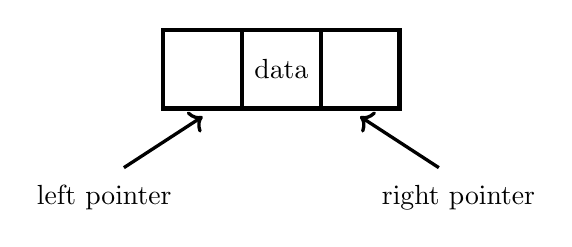
\begin{tikzpicture}
			[
				box/.style={rectangle,draw=black, ultra thick, minimum size=1cm},
			]
			
			\foreach \x/\y in {0/ , 1/\lr{data},2/ }
			\node[box] at (\x,0){\y};
			
			\draw[->,very thick] (-1,-1.25) --  node[above,xshift=-0.75cm,yshift=-1cm]{\lr{left pointer}} (0,-0.60);
			\draw[->,very thick] (3,-1.25) --  node[above,xshift=0.75cm,yshift=-1cm]{\lr{right pointer}} (2,-0.60);
		\end{tikzpicture}
	\end{minipage}%
	\begin{minipage}{0.5\textwidth}  % عکس در سمت راست
\begin{flushright}
\begin{latin}
\begin{lstlisting}
struct node{
	int data;
	struct node* left;
	struct node* right;
};
\end{lstlisting}
\end{latin}
\end{flushright}
\end{minipage}
\end{minipage}

\begin{question}
	
درخت رو به رو را به صورت لیست پیوندی پیاده سازی کنید.
\end{question}
\begin{answer}
در واقع هر فلش در شکل زیر یک اشاره گر از طرف گره والد است که به گره فرزند خود اشاره میکند.\\
\begin{latin}
		\begin{minipage}{0.35\textwidth}
			\begin{forest}
		for tree={
			circle, draw,
			scale=1.3,
			line width=1.5pt,
			minimum size=6mm,
			edge={
			line width=1.5pt,
			draw=black!70,
		},
	}
[A
	[B
		[D]
		[E]
	]
	[C]
]
\end{forest}
\end{minipage}%
\hfill
\begin{minipage}{0.9\textwidth}
\begin{forest}
for tree={
	edge={thick, -stealth},
	sacle=0.6
	l sep=1cm,
	s sep=1cm,
	node options={divided rectangle},
	align=center,
}
[A ,s sep=3cm
	[B, s sep=3cm
		[D]
		[E]
	]
	[C]
]
\end{forest}\\
\end{minipage}
\end{latin}
\end{answer}
پیاده سازی درخت با لیست پیوندی باعث می شود، خانه های خالی در آرایه نداشته باشیم.\\
بهتر است درخت های پر و کامل را با آرایه نمایش داده و درخت اریب را بهتر است به کمک لیست پیوندی نمایش دهیم.

\newpage

\subsection{پیمایش درخت دودویی}
پیمایش درخت یعنی حرکت روی یال های درخت و در این پیمایش باید با همه گره ها دقیقا یک بار ملاقات شود.\\


\textbf{روش های معمول پیمایش درخت دودویی}
\begin{enumerate}
	\item 
پیشوندی \lr{VLR} (ریشه - چپ - راست) ، این روش را \lr{preorder} می نامند.
	
	\item 
میانوندی \lr{LVR} (چپ - ریشه - راست ) ، این روش را \lr{inorder}می نامند.	
	\item 
پسوندی \lr{LRV} (چپ - راست - ریشه) این روش را \lr{postorder} می نامند.
\end{enumerate}

در پیمایش پیشوندی ابتدا ریشه ملاقات می شود، سپس زیر درخت سمت چپ به روش پیشوندی ملاقات می شود و در نهایت زیر درخت سمت راست به روش پیشوندی پیمایش می شود.\\

\begin{question}
سه روش پیمایش زیر را برای درخت زیر انجام دهید:
\end{question}
\begin{answer}
\begin{latin}
\begin{minipage}{0.65\textwidth}
		\begin{tabular}{c c c c c c c c c}
(VLR) & preorder: & J & E & A & H & T & M & Y \\
(LVR) & inorder:  & A & E & H & J & M & T & Y \\
(LRV) & postorder:& A & H & E & M & Y & T & J \\
		\end{tabular}
\end{minipage}%
\hfill
\begin{minipage}{0.35\textwidth}
\begin{forest}
for tree={
	scale=1.3,
	line width=1.5pt,
	minimum size=6mm,
	edge={
		line width=1.5pt,
		draw=black!70,
		},
}
[j
	[E
		[A]
		[H]
	]
	[T
		[M]
		[Y]
	]
]
\end{forest}
\end{minipage}
\end{latin}
\end{answer}

\begin{question}
پیمایش درخت زیر را با سه روش پیمایش درخت انجام دهید.
\end{question}
\begin{answer}
\begin{latin}
\begin{minipage}{0.7\textwidth}
\begin{tabular}{c c c c c c}
(VLR) & preorder:  & Y & T & W & Z \\
(LVR) & inorder:   & T & W & Y & Z \\
(LRV) & postorder: & W & T & Z & Y \\
\end{tabular}
\end{minipage}%
\hfill
\begin{minipage}{0.35\textwidth}
\begin{forest}
for tree={
	scale=1.3,
	line width=1.5pt,
	minimum size=6mm,
	edge={
		line width=1.5pt,
		draw=black!70,
		},
}
[Y
	[T
		[,phantom]
		[W]
	]
	[Z]
]
\end{forest}
\end{minipage}
\end{latin}
\end{answer}

\newpage

\begin{question}
	پیمایش درخت زیر را با سه روش پیمایش درخت انجام دهید.
\end{question}
\begin{answer}
\begin{latin}
\begin{minipage}{0.7\textwidth}
\begin{tabular}{c c c c c c c c}
(VLR) & preorder:  & S & R & Y & T & W & Z \\
(LVR) & inorder:   & R & S & T & W & Y & Z \\
(LRV) & postorder: & R & W & T & Z & Y & S \\
\end{tabular}
\end{minipage}%
\hfill
\begin{minipage}{0.35\textwidth}
\begin{forest}
for tree={
	scale=1.3,
	line width=1.5pt,
	minimum size=6mm,
	edge={
		line width=1.5pt,
		draw=black!70,
		 },
}
[S
	[R]
	[Y
		[T
			[,phantom]
			[W]
		]
		[Z]
	]	
]
\end{forest}
\end{minipage}
\end{latin}
\end{answer}

\begin{question}
سه روش پیمایش درخت دودویی را برای درخت زیر انجام دهید:
\end{question}
\begin{answer}
با توجه به گراف زیر داریم:\\
\begin{latin}
\begin{minipage}{0.8\textwidth}
\begin{small}
\begin{tabular}{c c c c c c c c c c c c c}
(VLR)& preorder: & P& F& B& H& G& S& R& Y& T& W& Z\\
(LVR)& inorder:  & B& F& G& H& P& R& S& T& W& Y& Z\\
(LRV)& postorder:& B& G& H& F& R& W& T& Z& Y& S& P\\
\end{tabular}
\end{small}
\end{minipage}%
\hfill
\begin{minipage}{0.3\textwidth}
\begin{forest}
for tree={
		scale=1,
		line width=1.5pt,
		minimum size=6mm,
		edge={
			line width=1.5pt,
			draw=black!70,
			 },
}
[P
	[F
		[B]
		[H
			[G]
			[,phantom]
		]
	]
	[S
		[R
			[T
				[,phantom]
				[W]
			]
		]
		[Y
			[,phantom]
			[Z]
		]
		
	]	
]
\end{forest}
\end{minipage}
\end{latin}
\end{answer}

\begin{question}
	پیمایش درخت زیر را با سه روش پیمایش درخت انجام دهید.
\end{question}
\begin{answer}
\begin{latin}
\begin{minipage}{0.7\textwidth}
\begin{tabular}{c c c c c c c c c c}
(VLR) & preorder:  & 8 & 5 & 3 & 4 & 2 & 6 & 1 & 9\\
(LVR) & inorder:   & 3 & 4 & 5 & 8 & 6 & 2 & 1 & 9\\
(LRV) & postorder: & 4 & 3 & 5 & 6 & 9 & 1 & 2 & 5\\
\end{tabular}
\end{minipage}%
\hfill
\begin{minipage}{0.35\textwidth}
\begin{forest}
for tree={
	scale=1.3,
	line width=1.5pt,
	minimum size=6mm,
	edge={
		line width=1.5pt,
		draw=black!70,
		 },
}
[8
	[5
		[3
			[,phantom]
			[4]
		]
		[,phantom]
	]
	[2
		[6]
		[1
			[,phantom]
			[9]
		]
	]
]			
\end{forest}
\end{minipage}
\end{latin}
\end{answer}
\newline
پیمایش یک درخت دودویی یک موضوع بازگشتی (\lr{recursive}) می باشد،
لذا برای انجام پیمایش  یک درخت ، باید پیمایش را برای زیر درخت ها انجام دهیم.

\newpage
\textbf{الگوریتم های پیمایش درخت دودویی}
\newline
الگوریتم های پیمایش درخت دودویی با سه حالت \lr{preorder} و 
\lr{inorder} و \lr{postorder} به صورت زیر می باشد:\\
توابع زیر همگی از نوع بازگشتی بوده و \lr{p} آدرس ریشه درخت دودویی می باشد.\\
\begin{center}
\begin{latin}
\begin{minipage}{0.5\textwidth}
\begin{lstlisting}
/////// preorder ///////
pre(p){
	if(p==null)	return;
	cout<< p->data;
	pre(p->left);
	pre(p->right);
}
\end{lstlisting}
\end{minipage}%
\hfill
\begin{minipage}{0.5\textwidth}
\begin{lstlisting}
/////// inorder ///////
in(p){
	if(p==null)	return;
	in(p->left);
	cout<< p->data;
	in(p->right);
}
\end{lstlisting}
\end{minipage}
\end{latin}
\end{center}

\begin{latin}
\begin{lstlisting}
/////// postorder ///////
post(p){
	if(p==null) return;
	post(p-<left);
	post(p->right);
	cout<<p->data
}
\end{lstlisting}
\end{latin}
\newpage

\subsection{رسم درخت دودویی}


\textbf{رسم درخت دودویی با داشتن پیمایش های پیشوندی و میانوندی}

\begin{question}
باتوجه به پیمایش های زیر ، درخت دو دویی را رسم کنید:
\begin{latin}
\begin{tabular}{c c c c c c c c}
preorder:& a & b & d & f & c & e & g \\
inorder: & d &f  & b & a & e & g & c \\
\end{tabular}
\end{latin}
\end{question}
\begin{answer}
برای رسم درخت باید مراحل زیر را انجام دهیم:
\begin{enumerate}
\item[گام اول)]
به دلیل وجود \lr{preorder} مشخص می شود که حرف اول در عبارت   \lr{preorder} یعنی \lr{a} ریشه درخت خواهد بود.\\
حال در عبارت \lr{inorder}، ریشه را پیدا می کنیم و عبارات سمت چپ و راست گراف مشخص خواهد شد.
	\begin{latin}
	\begin{minipage}{0.65\textwidth}
	\[
	inorder: \underbrace{dfb}_{\textrm{\rl{عبارت سمت چپ ریشه}}}
	\underbrace{a}_{\textrm{ریشه}}
	\underbrace{egc}_{\textrm{\rl{عبارت سمت راست ریشه}}}
	\]
	\end{minipage}%
	\hfill
	\begin{minipage}{0.35\textwidth}
	\begin{forest}
	for tree={
		circle, draw,
		scale=0.9,
		line width=1.5pt,
		minimum size=6mm,
		edge={
			line width=1.5pt,
			draw=black!70,
			 },
			}
	[a
		[dfb]
		[egc]
	]	
	\end{forest}
	\end{minipage}	
	\end{latin}

\item[گام دوم)]
حال باید به عبارت های چپ ریشه بپردازیم.\\
با مراجعه به عبارت \lr{preorder} باید گره های عبارت سمت چپ را بیابیم، می بینیم که بعد از \lr{a} ، \lr{b} قرار دارد لذا نتیجه می گیریم که برای عبارت سمت چپ، \lr{b} رشته می باشد.
	\begin{latin}
	\begin{forest}
	for tree={
		circle, draw,
		scale=0.9,
		line width=1.5pt,
		minimum size=6mm,
		edge={
			line width=1.5pt,
			draw=black!70,
		},
	}
	[a
		[b
			[df]
			[,phantom]
		]
		[,phantom]
	]	
\end{forest}
\end{latin}

\item[گام سوم)]
حال برای تعیین وضعیت دو گره \lr{d} و \lr{f} دوباره به عبارت \lr{preorder} مراجعه میکنیم و متوجه خواهیم شد که بعد از گره \lr{b} گره \lr{d} وجود دارد، درنتیجه \lr{d} ریشه ما نیست به \lr{f} خواهد بود و با نگاه به عبارت \lr{inorder} متوجه خواهیم شد که گره \lr{d} قبل از گره \lr{f} می باشد و گره \lr{f} فرزند راست گره \lr{d} خواهد بود.
\begin{latin}
		\begin{forest}
		for tree={
			circle, draw,
			scale=0.9,
			line width=1.5pt,
			minimum size=6mm,
			edge={
				line width=1.5pt,
				draw=black!70,
				 },
		}
		[a
			[b
				[d
					[,phantom]
					[f]
				]
				[,phantom]
			]
			[egc]
		]
		\end{forest}
\end{latin}

\item[گام چهارم)]
برای  تعیین وضعیت \lr{egc}، بعد از رسم کامل گره ها سمت چپ (\lr{dfb}) با مراجعه به عبارت \lr{preorder} و رسیدن به عبارت 
\lr{ceg} متوجه خواهیم شد که گره \lr{c}
ریشه می باشد.\\	
\begin{latin}
		\begin{forest}
			for tree={
				circle, draw,
				scale=0.9,
				line width=1.5pt,
				minimum size=6mm,
				edge={
					line width=1.5pt,
					draw=black!70,
				},
			}
			[a
				[b
					[d
						[,phantom]
						[f]
					]
					[,phantom]
				]
				[c
					[eg]
					[,phantom]
				]
			]	
		\end{forest}
\end{latin}

\item[گام پنجم)]
سپس برای وضعیت \lr{eg} با مراجعه به \lr{inorder}، متوجه خواهیم شد که \lr{eg} فبل از \lr{c} می باشد لذا \lr{eg} در چپ می باشد و با مراجعه به \lr{preorder} متوجه خواهیم شد که \lr{e} پدر گره \lr{g} خواهد بود و محل قرار گیری \lr{g} در سما راست استو\\
	\begin{latin}
		\begin{forest}
			for tree={
				circle, draw,
				scale=1.3,
				line width=1.5pt,
				minimum size=6mm,
				edge={
					line width=1.5pt,
					draw=black!70,
				},
			}
		[a
			[b
				[d
					[,phantom]
					[f]
				]
				[,phantom]
			]
			[c
				[e
					[,phantom]
					[g]
				]
				[,phantom]
			]
			
		]	
		\end{forest}
\end{latin}
\end{enumerate}
\end{answer}

\textbf{معمولا با داشتن دو پیمایش میتوان درخت را رسم کرد به شرط آنکه یکی از دو پیمایش ها \lr{inorder}} .باشد

\newpage

\textbf{مشخص کردن گره های تک فرزندی}

می توان به کمک دو پیمایش \lr{preorder} و \lr{postorder} یک درخت دودویی، گره های تک فرزندی را مشخص کرد.\\
برای اینکار در پیمایش \lr{preorder} از چپ به راست حرکت کرده و زوج پشت سرهمی که معکوس آن در پیمایش \lr{postorder} باشد را پیدا می کنیم، اولین گره در این زوج ها، گره تک فرزندی می باشد.\\
\begin{latin}
\begin{tabular}{c c c c c c c c c c}
	(VLR) & preorder:  & 8 & 5 & 3 & 4 & 2 & 6 & 1 & 9\\
	(LRV) & postorder: & 4 & 3 & 5 & 6 & 9 & 1 & 2 & 5\\
\end{tabular}
\end{latin}

با توجه به دو عبارت بالا به زوج های زیر می رسیم:
\[
(5,3), (3,4), (1,9)
\]
لذا در پیمایش \lr{preorder} ۳ جفت پیدا کردیم که معکوس آن در \lr{postorder} نیز می باشد.
\begin{center}
\begin{latin}
	\begin{forest}
		for tree={
			circle, draw,
			scale=0.7,
			line width=1.5pt,
			minimum size=6mm,
			edge={
				line width=1.5pt,
				draw=black!70,
			},
		}
	[8
		[5
			[3
				[,phantom]
				[4]
			]
			[,phantom]
		]
		[2
			[6]
			[1
				[,phantom]
				[9]
			]
		]
	]
	\end{forest}
\end{latin}
\end{center}

\subsection{درخت عبارت}
درخت عبارت از کاربرد های مهم درخت دودویی است که برای عبارت های ریاضی به کار می رود.\\
برگ های درخت حروف و عدد هستند و گره های غیر برگ عملگر می باشند.
\[
A - (C\div 3\times2) + (D\times5 \% 4)
\]


\begin{minipage}{0.7\textwidth}
\begin{flushright}
\begin{itemize}
			\item 
پیمایش \lr{inorder} یک درخت عبارت، نگارش \lr{infix} را تولید می کند.
			\item 
			پیمایش \lr{preorder} یک درخت عبارت، نگارش \lr{prefix} را تولید می کند.
			\item 
			پیمایش \lr{postorder} یک درخت عبارت، نگارش \lr{postfix} را تولید می کند.	
\end{itemize}
\end{flushright}
\end{minipage}%
\begin{minipage}{0.4\textwidth}
\begin{latin}
\begin{forest}
	for tree={
		circle, draw,
		scale=1,
		line width=1.5pt,
		minimum size=6mm,
		edge={
			line width=1.5pt,
			draw=black!70,
			-- %
		},
	}
	[+
		[-
			[A]
			[*
				[/
					[C]
					[5]
				]
				[2]
			]
		]
		[\%
			[*
				[D]
				[5]
			]
			[4]
		]
	]	
\end{forest}
\end{latin}
\end{minipage}



\newpage
\textbf{تعداد درخت های دودویی که می توان به \lr{n} گره ساخت}\\
فرض می کنیم هر یک از گره ها را به روش \lr{inorder} از ۱ تا \lr{n} شماره گذاری کرده ایم:\\
اگر گره شماره \lr{i} ریشه باشد، در آن صورت \lr{i-1} گره در زیر درخت چپ ریشه و \lr{n-i} گره در زیر درخت راست ریشه قرار دارد:\\
\[
1,2,3,\dots,i-1,i,i+1,\dots,n
\]

\[
\underbrace{b_n}_{\textrm{\rl{تعداد درخت ها}}}  = \sum_{i=1}^{n} b_{i-1} b_{n-i}
\]

\[
b_0 = 1 , b_1 = 1
\]

\textbf{رسم درخت دودویی با داشتن پیمایش های پیشوندی و پسوندی}\\

اگر پیمایش های پیشوندی و پسوندی یک درخت دمودویی در دسترس باشند، محل گره های تک فرزندی را نمی توان مشخص کرد.\\
بنابر این در صورت وجود گره های تک فرزندی ، چندین درخت می توان ایجاد کرد که پیمایش \lr{preorder} و \lr{postorder} آنها باهم برابر باشند.\\
این درخت ها برابر است با$2^k$ که در آن \lr{k} تعداد گره های تک فرزندی است.\\
\begin{question}
با توجه به \lr{preorder} و \lr{postorder} بیان شده، درخت را رسم کنید:
\begin{latin}
\begin{tabular}{c c c c c c c c c c c}
(VLR) & preorder:  & A & B & C & D & E & F & G & H & I \\
(LRV) & postorder: & C & E & D & B & H & I & G & H & A \\
\end{tabular}
\end{latin}
\end{question}

\begin{answer}
با توجه به اینکه \lr{k} تعداد گره های تک فرزندی است لذا 
$2^2 = 4$
حالت داریم که گره های تک فرزندی آن ها مشخص است.

\begin{center}
\begin{latin}
\begin{tabular}{|c|c|c|c|}
\hline
\begin{latin}
\begin{forest}
for tree={
	circle, draw,
	scale=0.6,
	line width=1.5pt,
	minimum size=6mm,
	edge={
		line width=1.5pt,
		draw=black!70,
		},
}
[A
	[B
		[C]
		[D
			[,phantom]
			[E]
		]
	]
	[F
		[,phantom]
		[G
			[H]
			[I]
		]
	]
]
\end{forest}
\end{latin}&
\begin{latin}
\begin{forest}
for tree={
	circle, draw,
	scale=0.6,
	line width=1.5pt,
	minimum size=6mm,
	edge={
		line width=1.5pt,
		draw=black!70,
		},
}
[A
	[B
		[C]
		[D
			[,phantom]
			[E]
		]
	]
	[F
		[G
			[H]
			[I]
		]
		[,phantom]
	]	
]
\end{forest}
\end{latin}&
\begin{latin}
\begin{forest}
for tree={
	circle, draw,
	scale=0.6,
	line width=1.5pt,
	minimum size=6mm,
	edge={
		line width=1.5pt,
		draw=black!70,
		},
}
[A
	[B
		[C]
		[D
			[E]
			[,phantom]
		]
	]
	[F
		[,phantom]
		[G
			[H]
			[I]
		]
	]
]
\end{forest}
\end{latin}&
\begin{latin}
\begin{forest}
for tree={
	circle, draw,
	scale=0.6,
	line width=1.5pt,
	minimum size=6mm,
	edge={
		line width=1.5pt,
		draw=black!70,
		},
}
[A
	[B
		[C]
		[D
			[E]
			[,phantom]
		]
	]
	[F
		[G
			[H]
			[I]
		]
		[,phantom]
	]
]
\end{forest}\\
\hline
\end{tabular}
\end{latin}
\end{center}
\end{answer}


\subsection{درخت کلی (عمومی)}
با فرض اینکه یک گره دارای یک فرزند باشد، آنگاه این فرزند در یک درخت دودویی با عنوان بچه چپ یا راست از هم متمایز می شوند، اما در یک درخت کلی تفاوتی بین آنها وجود ندارد.\\
برای پیاده سازی درخت های کلی، آنها را به صورت یک درخت دودویی در می آوریم که به آن (درخت دودویی معادل) با درخت اصلی می گوییم.
\begin{center}
\begin{latin}
\begin{forest}
for tree={
	circle, draw,
	scale=1.3,
	line width=1.5pt,
	minimum size=6mm,
	edge={
		line width=1.5pt,
		draw=black!70,
		-> %
		},
}
[A
	[B]
		[C
			[E]
			[F]
		]
	[D]
]
\end{forest}
\end{latin}
\end{center}

\textbf{مراحل تبدیل یک درخت به درخت دودویی معادل}\\
برای تبدیل فوق باید مراحل زیر را به ترتیب انجام دهیم.\\
\begin{enumerate}
	\item[مرحله اول)] 
	در هر سطح باید کلیه گره های کنار هم (فرزندان یک پدر) را به یکدیگر متصل کنیم.
\begin{center}
\begin{latin}
\begin{forest}
for tree={
	circle, draw,
	scale=1.3,
	line width=1.5pt,
	minimum size=6mm,
	edge={
		line width=1.5pt,
		draw=black!70,
		-> %
		},
}
[A
	[B]
		[C
			[E]
			[F]
		]
	 	[D]
]
\end{forest}
\end{latin}
\end{center}

\newpage

\item[مرحله دوم)] 
کلیه اتصالات گره را به گره پدر، به جز اتصال سمت چپ ترین فرزند را قطع می کنیم.\\

\begin{center}
\begin{latin}
	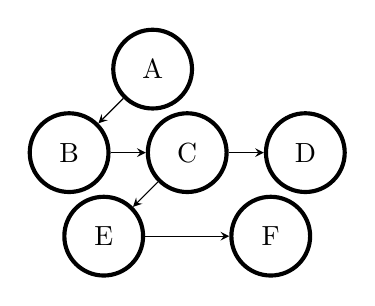
\begin{tikzpicture}[->, >=stealth, node distance=1.5cm, 
			every node/.style={draw, circle,line width=1.5pt, minimum size=1cm}]
			
			\node (A) {A};
			\node (B) [below left of=A] {B};
			\node (C) [right of=B] {C};
			\node (D) [right of=C] {D};
			\node (E) [below left of=C] {E};
			\node (F) [below right of=C] {F};
			\draw (A) -- (B);
			\draw (B) -- (C);
			\draw (C) -- (D);
			\draw (C) -- (E);
			\draw (E) -- (F);
	\end{tikzpicture}
\end{latin}
\end{center}
\end{enumerate}

\textbf{اولین فرزند هر گره در درخت اصلی،
فرزند چپ آن در درخت دودویی معادل است و برادر سمت راست هر گره در درخت اصلی فرزند راست آن، در درخت معادل است.
}

\subsection{جنگل \lr{Forest}} 
چند درخت کلی اگر کنار هم قرار گیرند، تشکیل یک جنگل می دهند.\\
به عبارت دیگر جنگل شامل \lr{n} درخت مجزا است (\lr{n >= 0})

\begin{center}
\begin{latin}
\begin{tabular}{|ccc|}
\hline
\begin{latin}
\begin{forest}
for tree={
	circle, draw,
	scale=1.3,
	line width=1.5pt,
	minimum size=6mm,
	edge={
		line width=1.5pt,
		draw=black!70,
		-> %
		},
}
[A,label=above:Forest
	[B]
	[C]
	[D]	
]
\end{forest}
\end{latin}&
\begin{latin}
\begin{forest}
for tree={
	circle, draw,
	scale=1.3,
	line width=1.5pt,
	minimum size=6mm,
	edge={
		line width=1.5pt,
		draw=black!70,
		-> %
		},
}
[E[F]]
\end{forest}
\end{latin}&
\begin{latin}
\begin{forest}
for tree={
	circle, draw,
	scale=1.3,
	line width=1.5pt,
	minimum size=6mm,
	edge={
		line width=1.5pt,
		draw=black!70,
		-> %
		},
}
[G
	[H]
	[I]
]
\end{forest}
\end{latin}\\
\hline
\end{tabular}
\end{latin}
\end{center}

\textbf{تبدیل جنگل به درخت دودویی}\\
برای تبدیل فوق باید مراحل زیر را به ترتیب انجام دهیم.\\
\begin{enumerate}
	\item[مرحله اول)] 
هر درخت جنگل را به یک درخت دودویی تبدیل می کنیم.
\begin{center}
\begin{latin}
\begin{tabular}{|ccc|}
\hline
\begin{latin}
\begin{forest}
for tree={
circle, draw,
scale=1.3,
line width=1.5pt,
minimum size=6mm,
edge={
	line width=1.5pt,
	draw=black!70,
-> %
	},
}
[A,label=above:Forest
	[B]
		[C]
		[D]	
]
\end{forest}
\end{latin}&
\begin{latin}
\begin{forest}
for tree={
	circle, draw,
	scale=1.3,
	line width=1.5pt,
	minimum size=6mm,
	edge={
		line width=1.5pt,
		draw=black!70,
		-> %
		},
}
[E[F]]
\end{forest}
\end{latin}&
\begin{latin}
\begin{latin}
\begin{forest}
for tree={
	circle, draw,
	scale=1.3,
	line width=1.5pt,
	minimum size=6mm,
	edge={
		line width=1.5pt,
		draw=black!70,
		-> %
		},
}
[G
	[H]
	[I]
]
\end{forest}
\end{latin}\\
\hline
\end{tabular}
\end{latin}
\end{center}
\newpage
\item[مرحله دوم)] 
درخت های دودویی را از طریق فرزند راست گره های ریشه به هم متصل می کنیم.
\begin{center}
\begin{latin}
\begin{forest}
for tree={
	circle, draw,
	scale=1.3,
	line width=1.5pt,
	minimum size=6mm,
	edge={
		line width=1.5pt,
		draw=black!70,
		-> %
		},
}
[A
	[B
		[,phantom]
		[C
			[,phantom]
			[D]
		]
	]
	[E
		[F]
		[G	
			[H
				[,phantom]
				[I]
			]		
			[,phantom]
		]
	]
]
\end{forest}
\end{latin}
\end{center}
\end{enumerate}
\textbf{در درخت دودویی حاصل از جنگل، تعداد برگ ها ، 
برابر تعداد درخت هایی است که جنگل را تشکیل داده اند.
}

\newpage

\subsection{پیاده سازی الگوریتم های مربوط به درخت}

\textbf{ساختار یک گره یک درخت دودویی}\\
\begin{flushright}
	\begin{latin}
\begin{lstlisting}
struct node{int data;struct node* left; struct node* right; };
\end{lstlisting}
	\end{latin}
\end{flushright}


\textbf{تابع \lr{newnode}}\\
این تابع برای ایجاد گره های متعدد برای یک درخت می باشد.\\
\begin{flushright}
	\begin{latin}
\begin{lstlisting}
struct node* newnode(int item){
	struct node* node = (struct node*) malloc(sizeof(struct node)); (1)
	node->data = item;  (2)
	node->left = Null;  (3)
	node->right = Null; (4)
	return node;
}
\end{lstlisting}
\end{latin}
\end{flushright}
\begin{enumerate}
	\item[\lr{(1)}]
	با دستور \lr{malloc} دریافت یک فضای خالی از حافظه به اندازه یک \lr{node} را انجام می دهیم.
	\item[\lr{(2)}]
	در قسمت \lr{data} ، \lr{node} ایجاد شده، مقدار \lr{item} را قرار بده.
	\item[\lr{(3,4)}]
	در دو قسمت \lr{left} و \lr{right} گره ایجاد شده، که برای آدرس دهی ماست \lr{Null} را قرار بده.\\
\end{enumerate}

\textbf{شمارش تعداد گره ها }\\
این تابع آدرس ریشه یک درخت را می گیرد و تعداد گره های درخت را بر می گرداند.
\begin{flushright}
\begin{latin}
\begin{lstlisting}
unsigned int count(struct node* root){
	if(root = Null)
		return (0);
	return (1 + count(root->left) + count(root->right));
}			
\end{lstlisting}
\end{latin}
\end{flushright}
این تابع به صورت بازگشتی شمارش تعداد گره های یک درخت دودویی را انجام می دهد.\\
\newpage
\textbf{تشخیص برگ بودن}\\
این تابع برای تشخیص برگ بود می باشد، به تابع زیر یک گره به عنوان ورودی میدهیم و تشخصی می دهد که گره برگ است یا خیر.
\begin{flushright}
\begin{latin}
\begin{lstlisting}
bool isleaf(struct node* n){
	if(n==Null)
		return false;
	if((n->left==Null) && (n->right==Null))
		return true;
	return false;
}	
\end{lstlisting}
\end{latin}
\end{flushright}

\begin{question}
با توجه به الگوریتم های بیان شده درخت زیر را ایجاد کنید.
\end{question}
\begin{answer}
	با توجه به درخت زیر داریم:
\begin{latin}
\begin{minipage}{0.7\textwidth}
\begin{flushright}
	\begin{latin}
\begin{lstlisting}
int main(void){
	struct node* nr = Null;
	struct node* root = newnode(2)
	root->left = newnode(7);
	root->right = newnode(5);
	root->left->right = newnode(6);
	root->left->right->left = newnode(1);
	root->right->right = newnode(9);
}
\end{lstlisting}
	\end{latin}
\end{flushright}
		\end{minipage}%
\hfill
\begin{minipage}{0.35\textwidth}
\begin{forest}
for tree={
	scale=1.3,
	line width=1.5pt,
	minimum size=6mm,
	edge={
		line width=1.5pt,
		draw=black!70,
		},
}
[2
	[7
		[,phantom]
		[6
			[1]
			[,phantom]
		]
		
	]
	[5
		[,phantom]
		[9]
	]
]
\end{forest}
\end{minipage}
\end{latin}
\end{answer}

\textbf{تشخیص کامل بودن درخت دودویی}\\
تابع زیر تشخیص می دهد که درخت دودویی کامل است یا خیر.
\begin{flushright}
\begin{latin}
\begin{lstlisting}
bool f(struct node* root, unsigned int i, unsigned int n){
	if(root == Null)
		retrun (true);
	if(i>n)
		return false;
	return(f(root->left, 2*i, n) && f(root->right, 2i+1, n))
}
\end{lstlisting}
\end{latin}
\end{flushright}
این تابع نیز به صورت بازگشتی بررسی می کند که یک درخت کامل است یا خیر.
\newpage

\textbf{حذف گره های تک فرزندی}\\
تابع زیر گره های تک فرزندی یک درخت را به صورت بازگشتی حذف می کند.
\begin{flushright}
\begin{latin}
\begin{lstlisting}
struct node* remove(struct node* root){
	if(root==NUll) return Null;
	root->left = remove(root->left);
	root->right = remove(root->right);
	 if((root->left==Null) && (root->right==NUll))
		return root;
	if(root->left==Null)
		{struct node* n = root->right;free(root):return n;}
	if(root->right==Null)
		{struct node* n = root->left;free(root):return n;}
}	
\end{lstlisting}
\end{latin}
\end{flushright}
\textbf{پیاده سازی درخت در صف}

\begin{flushright}
ایجاد صف برای پیاده سازی درخت
\begin{latin}
\begin{lstlisting}
struct node** createQueue(int *front, int *rear){
	struct node** queue = (struct node**)malloc(sizeof(struct node*)*Max);
	*front = *rear = 0;
	return queue;
}
\end{lstlisting}
\end{latin}
\end{flushright}
\begin{flushright}
دریافت گره (مقدار) برای درج در صف
\begin{latin}
\begin{lstlisting}
void enQueue(struct node **queue, int *rear,struct node* newnode){
	queue[*rear] = newnode;
	(*rear)++;
}
\end{lstlisting}
\end{latin}
\end{flushright}
\begin{flushright}
حذف گره از صف (حذف گره)
\begin{latin}
\begin{lstlisting}
struct node* deQueue(struct node **queue, int *front){
	(*front)++;
	return queue[*front-1]
}
\end{lstlisting}
\end{latin}
\end{flushright}




\section{گراف}
گراف \lr{G = (V,E)} مجموعه ای از راس و یال است.\\
\begin{tabular}{c c}
\lr{V} :  گره ،  مجموعه محدود و غیر تهی از رئوس 
&
\lr{E} : یال ، مجموعه از زوج رئوس \\ 	
\end{tabular}\\
\newline
\textbf{انواع گراف}
\begin{enumerate}
	\item 
جهت دار:\\
ترتیب گره ها در زوج مرتب اهمیت دارد.
	\item 
غیر جهت دار:\\
گرافی که در آن جای دو راس در مجموعه یال ها اهمیت نداشته باشد.\\
\end{enumerate}
درجه یک گره به معنی یال هایی است که به یک گره برخورد می کند می باشد.\\
برای محاسبه تعداد کل یال ها همه درجه ها را با هم جمع کرده و تقسیم برای ۲ میکنیم .\\
به طور مثال در زیر دو گراف داریم که به ترتیب  بدون جهت و جهت دارد می باشند.\\
استفاده از مجموعه به معنی این است که گراف بدون جهت می باشد و استفاده از پرانتز برای یال های یا به معنی جهت دار بودن گراف می باشد.
\begin{center}
\begin{minipage}{0.5\textwidth}
\[
V = \{a, b, c, d\}
\]
\[
E = \{\{a,b\}, \{a,c\}, \{b,c\}, \{b,d\}, \{c,d\}\}
\]
\begin{latin}
\begin{tikzpicture}[scale=0.7,
	every node/.style={circle, draw, minimum size=8mm}
	]
	\node[label=left:{deg(a)=2}] (a) at (0,2) {a};
	\node[label=right:{deg(b)=3}] (b) at (3,2) {b};
	\node[label=below left:{deg(c)=3}] (c) at (0,0) {c};
	\node[label=below right:{deg(d)=2}] (d) at (3,0) {d};
	\draw[--, thick] (a) to (b); 
	\draw[--, thick] (a) to	(c);  
	\draw[--, thick] (c) to (b); 
	\draw[--, thick] (c) to	(d);  
	\draw[--, thick] (b) to	(d);  
\end{tikzpicture}
\end{latin}
\end{minipage}%
\hfill
\begin{minipage}{0.5\textwidth}
\[
V = \{a,b,c\}
\]
\[
E = \{(a,c), (a,b), (b,c), (c,b)\}
\]
\begin{latin}
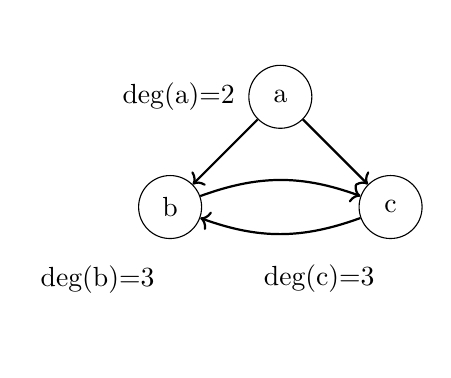
\begin{tikzpicture}[scale=0.7,
	every node/.style={circle, draw, minimum size=8mm}
	]
	\node[label=left :{deg(a)=2}] (a) at (2,2) {a};
	\node[label=below left:{deg(b)=3}] (b) at (0,0) {b};
	\node[label=below left:{deg(c)=3}] (c) at (4,0) {c};

	\draw[->, thick] (a) to (b); 
	\draw[->, thick] (a) to	(c);  
	\draw[->, thick] (c) to [bend left=20] (b); 
	\draw[->, thick] (b) to [bend left=20] (c);  
\end{tikzpicture}
\end{latin}
\end{minipage}
\end{center}
می توانیم برای گراف جهت دار درجه ها را نیز تفکیک کنیم یعنی داشته باشیم :\\
$deg^+$ اشاره به یال خروجی از یک گره\\
$deg^-$ اشاره به یال های ورودی یک گره\\

در حالت  \lr{deg} اشاره به درجه کل گره می باشد ، یعنی جمع تمام گره های ورودی و خروجی از یک گره.\\
\begin{center}
\begin{latin}
	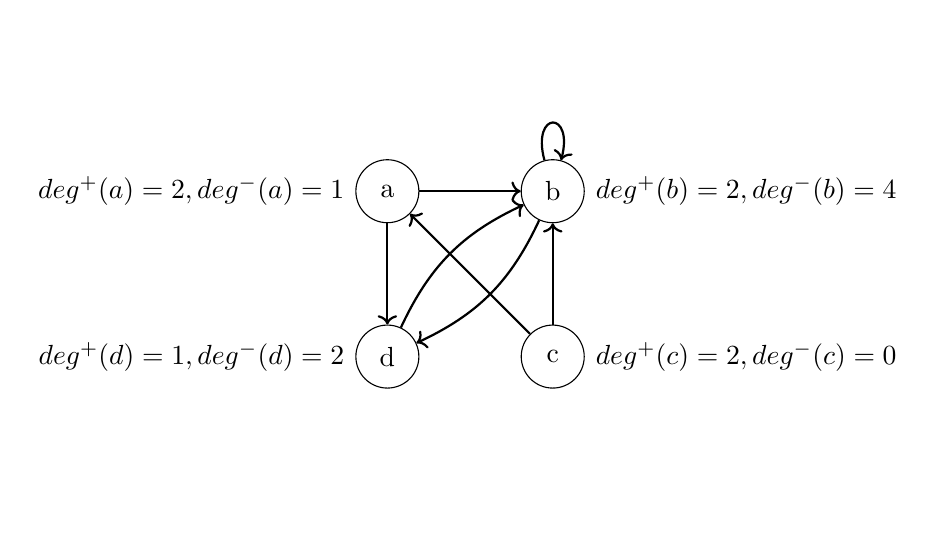
\begin{tikzpicture}[scale=0.7,
		every node/.style={circle, draw, minimum size=8mm}
		]
		\node[label=left:{$deg^+(a) = 2, deg^-(a) = 1$}] (a) at (0,3) {a};
		\node[label=right:{$deg^+(b) = 2, deg^-(b) = 4$}] (b) at (3,3) {b};
		\node[label=right:{$deg^+(c) = 2, deg^-(c) = 0$}] (c) at (3,0) {c};
		\node[label=left:{$deg^+(d) = 1, deg^-(d) = 2$}] (d) at (0,0) {d};
		\draw[->, thick] (a) to (b);
		\draw[->, thick] (b) to [loop above] (b); 
		\draw[->, thick] (a) to	(d);  
		\draw[->, thick] (c) to	(a);
		\draw[->, thick] (c) to	(b);  
		\draw[->, thick] (b) to [bend left=20] (d); 
		\draw[->, thick] (d) to [bend left=20] (b);  
	\end{tikzpicture}
\end{latin}
\end{center}

\textbf{گراف چند گانه}\\
گرافی که در آن یال های چند گانه مجاز باشد را گراف چند گانه یا (\lr{multiEdge}) می گویند.

\begin{latin}
	\begin{tikzpicture}[scale=0.7,
		every node/.style={circle, draw, minimum size=8mm}
		]
		\node (1) at (0,4) {1};
		\node (2) at (0,2) {2};
		\node (3) at (0,0) {3};
		\node (4) at (4,2) {4};
		\draw[--, thick] (1) to (2); 
		\draw[--, thick] (2) to	(3);  
		\draw[--, thick] (2) to	(4); 
		\draw[--, thick] (2) to [bend left=20] (4); 
		\draw[--, thick] (3) to [bend right=20] (4);  
		\draw[--, thick] (3) to [bend right=30] (4); 
		\draw[--, thick] (3) to [bend right=40] (4);  
	\end{tikzpicture}
\end{latin}
\end{center}

\textbf{گراف کامل}\\
گراف بدون جهتی که همه یال های آن رسم شده باشند.\\
درجه هر یک از گره ها: $n-1$ \\
تعداد یال ها: $\frac{n(n-1)}{2}$ \\
به طور مثال گراف زیر ۴ راس دارد که هر راس به راس دیگر وصل است:
\begin{center}
\begin{latin}
\begin{tikzpicture}[scale=0.7,
	every node/.style={circle, draw, minimum size=8mm}
	]
	\node (a) at (0,3) {a};
	\node (b) at (3,3) {b};
	\node (c) at (0,0) {c};
	\node (d) at (3,0) {d};
	\draw[--, thick] (a) to (b); 
	\draw[--, thick] (a) to	(c);  
	\draw[--, thick] (a) to (d); 
	\draw[--, thick] (c) to	(d);  
	\draw[--, thick] (c) to	(b);  
	\draw[--, thick] (d) to	(b);   
\end{tikzpicture}
\end{latin}
\end{center}

\newpage
\textbf{گراف هم بند}\\
گرافی که یک مسیر بین هر دو گره آن وجود داشته باشد.\\
به طور مثال شکل زیر یک گراف ناهمبند است:
\begin{center}
	\begin{latin}
		\begin{tikzpicture}[scale=0.5,
			every node/.style={circle, draw, minimum size=4mm}
			]
			\node (a) at (2,4) {a};
			\node (b) at (0,0) {b};
			\node (c) at (4,0) {c};
			\node (d) at (5,4) {d};
			\node (e) at (2,2) {e};
			\draw[--, thick] (a) to (b); 
			\draw[--, thick] (a) to	(c);  
			\draw[--, thick] (b) to (c); 
			\draw[--, thick] (e) to (d);    
		\end{tikzpicture}
	\end{latin}
\end{center}
گراف هم بند قوی:\\
گرافی جهت داری که برای هر زوج گره \lr{v,u}، هم یک مسیر از \lr{u}
به \lr{v} و هم یک مسیر از \lr{v} به \lr{u} وجود داشته باشد.\\


\subsection{نمایش گراف}
\begin{enumerate}
	\item
ماتریس همجواری (همسایگی) \lr{Adjacency Matrices}
	\item
لیست همجواری  \lr{Adjacency List} \\

\end{enumerate}

\textbf{ماتریس همجواری}\\
با ذکر دو مثال ماترس همجواری را برای دو گراف جهت دار و بدون جهت شرح میدهیم.\\
\begin{question}
نمایش ماتریس همجواری گراف بدون جهت زیر:
\end{question}
\begin{answer}
با توجه به گراف روبه رو داریم:
\begin{latin}
	\begin{minipage}{0.45\textwidth}
		\centering
		\begin{tikzpicture}[scale=0.7,
	every node/.style={circle, draw, minimum size=8mm}
	]
	\node (e) at (0,0) {e};
	\node (d) at (2,0) {d};
	\node (b) at (4,0) {b};
	\node (a) at (3,2) {d};
	\node (c) at (3,-2) {c};
	\draw[--, thick] (e) to (d); 
	\draw[--, thick] (d) to	(b);  
	\draw[--, thick] (d) to (a); 
	\draw[--, thick] (a) to (b);
	\draw[--, thick] (c) to (a);    
\end{tikzpicture}
	\end{minipage}%
	\hfill
	\begin{minipage}{0.55\textwidth}
\[
\begin{array}{c|cccccc}
		  & a & b & c & d  & e  \\ 
	\hline
	a     & 0 & 1 & 1 & 1  & 0  \\
	b     & 1 & 0 & 0 & 1  & 0  \\
	c     & 1 & 0 & 0 & 0  & 0  \\
	d     & 1 & 1 & 0 & 0  & 1  \\
	e     & 0 & 0 & 0 & 1  & 0  \\
\end{array}
\]
\end{minipage}
\end{latin}
\begin{enumerate}
	\item[مرحله اول)]
ماتریس ایجاد می کنیم به اندازه سطر و ستون تعداد گره های گراف و سپس به بررسی وضعیت یال های هر گره می پردازیم. 
	\item[مرحله دوم)]
گره \lr{a} با سه گره \lr{b,c,d} همجوار است لذا سطر مربوط در ماتریس را ۱ قرار داده و مابقی خانه ۰ می شوند.\\
گره \lr{b} با گره \lr{a,d} همجوار است لذا سطر های مربوطه در ماتریس ۱ می شوند و مابقی درایه ها .
\end{enumerate}
به همین ترتیب عمل فوق را برای هر گره تکرار کرده تا جدول کامل شود و به ماتریس همجواری برسیم.\\
\end{answer}
\newpage
\begin{question}
	نمایش ماتریس همجواری گراف جهت دار زیر:
\end{question}
\begin{answer}
	با توجه به گراف روبه رو داریم:
	\begin{latin}
		\begin{minipage}{0.45\textwidth}
			\centering
			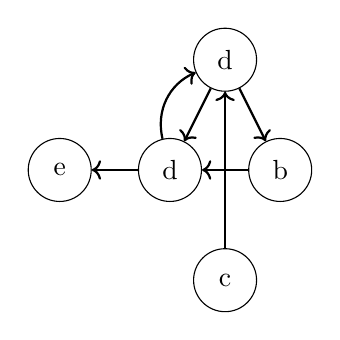
\begin{tikzpicture}[scale=0.7,
				every node/.style={circle, draw, minimum size=8mm}
				]
				\node (e) at (0,0) {e};
				\node (d) at (2,0) {d};
				\node (b) at (4,0) {b};
				\node (a) at (3,2) {d};
				\node (c) at (3,-2) {c};
				\draw[->, thick] (d) to (e); 
				\draw[->, thick] (a) to	(b);  
				\draw[->, thick] (d) to [bend left=40] (a); 
				\draw[->, thick] (a) to (d);
				\draw[->, thick] (c) to (a);
				\draw[->, thick] (b) to (d);    
			\end{tikzpicture}
		\end{minipage}%
		\hfill
		\begin{minipage}{0.55\textwidth}
			\[
			\begin{array}{c|cccccc}
				& a      &  b     &    c   &    d   & e  \\ \hline
				a     & 0 & 1 & 0 & 1  & 0  \\
				b     & 0 & 0 & 0 & 1  & 0  \\
				c     & 1 & 0 & 0 & 0  & 0  \\
				d     & 1 & 0 & 0 & 0  & 1  \\
				e     & 0 & 0 & 0 & 0  & 0  \\
			\end{array}
			\]
		\end{minipage}
	\end{latin}
	\begin{enumerate}
		\item[مرحله اول)]
		ماتریس ایجاد می کنیم به اندازه سطر و ستون تعداد گره های گراف و سپس به بررسی وضعیت یال های هر گره می پردازیم ، با این تفاوت که مبانی ۱ شدن درایه ماتریس در این است که از گره مد نظر ما باید یالی خارج شده باشد.\\
و در غیر اینصورت یعنی اگر یالی وجود نداشته باشد یا یال به گره وارد شده باشه در درایه مربوطه ۰ قرار میدهیم.
		\item[مرحله دوم)]
گره \lr{a} با سه گره \lr{b,d} همجوار است لذا سطر مربوط در ماتریس را ۱ قرار می دهیم و مابقی داریه ها ۰ می شوند.\\
گره \lr{b} با گره \lr{d} همجوار است لذا درایه مربوطه در ماتریس ۱ می شوند و مابقی درایه ها . می شوند.
	\end{enumerate}
به همین ترتیب عمل فوق را برای هر گره تکرار کرده تا جدول کامل شود و به ماتریس همجواری برسیم.\\
\end{answer}

\textbf{لیست همجواری}\\
لیست همجواری را نیز همانند ماتریس همجواری با ذکر دو مثال شرح می دهیم .
\begin{question}
نمایش  همجواری گراف بدون جهت زیر:
\end{question}
\begin{answer}
با توجه به گراف روبه رو داریم:
\begin{latin}
	\begin{minipage}{0.45\textwidth}
		\centering
\begin{tikzpicture}[scale=0.7,
every node/.style={circle, draw, minimum size=8mm}
			]
\node (e) at (0,0) {e};
\node (d) at (2,0) {d};
\node (b) at (4,0) {b};
\node (a) at (3,2) {d};
\node (c) at (3,-2) {c};
\draw[--, thick] (e) to (d); 
\draw[--, thick] (d) to	(b);  
\draw[--, thick] (d) to (a); 
\draw[--, thick] (a) to (b);
\draw[--, thick] (c) to (a);    
\end{tikzpicture}
\end{minipage}%
\hfill
\begin{minipage}{0.55\textwidth}
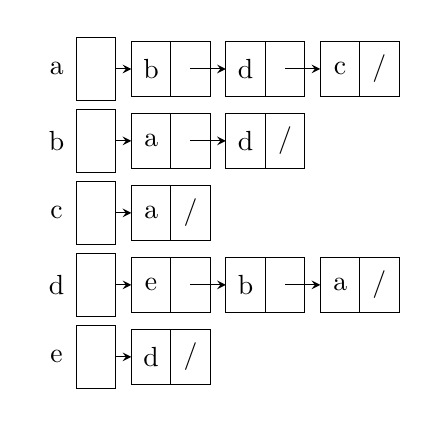
\begin{tikzpicture}[>=stealth] 
	\matrix (M) [matrix of nodes,% 
	column sep=-\pgflinewidth,% 
	row sep=1mm,% 
	nodes in empty cells,
	nodes={draw,%
		minimum width=.5cm, outer sep=0pt,% 
		minimum height=.7cm, anchor=center}, 
	column 1/.style={nodes={minimum height=.8cm}}]%
	{ 
|[label=left:a]| &[2mm] b & &[2mm] d & &[2mm] c &/  \\ 
|[label=left:b]| &[2mm] a & &[2mm] d &/  \\ 
|[label=left:c]| &[2mm] a &/  \\ 
|[label=left:d]| &[2mm] e & &[2mm] b & &[2mm] a & /  \\ 
|[label=left:e]| &[2mm] d &/  \\
	}; 
	
	\foreach \i in {1,2,3,4,5}{ 
 		\draw[->] (M-\i-1)--(M-\i-2.west); 
	}
	\foreach \i in {1,4}{ 
		\draw[->] (M-\i-3.center)--(M-\i-4.west);
		\draw[->] (M-\i-5.center)--(M-\i-6.west);	
}
\draw[->] (M-2-3.center)--(M-2-4.west); 
\end{tikzpicture} 
\end{minipage}
\end{latin}
\newpage

\begin{enumerate}
	\item[مرحله اول)]
برای هر گره موجود در گراف لیست ای در نظرم می گیرم.\\
سپس لیست همجواری بدین صورت است که گره مد نظر به هر گره دیگری یال داشت، آنرا در یک خانه لیست مربوط به گره می نویسیم .
	\item[مرحله دوم)]
	گره \lr{a} با سه گره \lr{c,b,d} همجوار است، لذا درون آرایه \lr{a} نام این سه گره را درج میکنیم.\\
	گره \lr{b} با گره های \lr{a,d} همجوار است لذا در لیست مربوط به \lr{b} این اسامی را قرار می دهیم.\\
	کار را به همین ترتیب ادامه داده یا همه لیست همه گره ها کامل شود.\\
\end{enumerate}

\begin{question}
	نمایش لیست همجواری گراف  جهت دار :
\end{question}
\begin{answer}
	با توجه به گراف روبه رو داریم:
\begin{latin}
\begin{minipage}{0.45\textwidth}
	\centering
	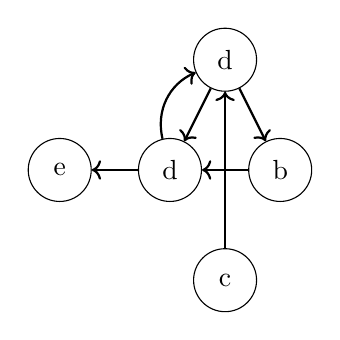
\begin{tikzpicture}[scale=0.7,
		every node/.style={circle, draw, minimum size=8mm}
		]
		\node (e) at (0,0) {e};
		\node (d) at (2,0) {d};
		\node (b) at (4,0) {b};
		\node (a) at (3,2) {d};
		\node (c) at (3,-2) {c};
		\draw[->, thick] (d) to (e); 
		\draw[->, thick] (a) to	(b);  
		\draw[->, thick] (d) to [bend left=40] (a); 
		\draw[->, thick] (a) to (d);
		\draw[->, thick] (c) to (a);
		\draw[->, thick] (b) to (d);    
\end{tikzpicture}
\end{minipage}%
\hfill
\begin{minipage}{0.55\textwidth}
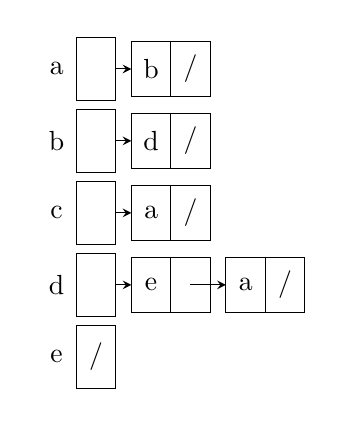
\begin{tikzpicture}[>=stealth] 
				\matrix (M) [matrix of nodes,% 
				column sep=-\pgflinewidth,% 
				row sep=1mm,% 
				nodes in empty cells,
				nodes={draw,%
					minimum width=.5cm, outer sep=0pt,% 
					minimum height=.7cm, anchor=center}, 
				column 1/.style={nodes={minimum height=.8cm}}]%
				{ 
					|[label=left:a]| &[2mm] b & /  \\ 
					|[label=left:b]| &[2mm] d & /  \\ 
					|[label=left:c]| &[2mm] a & /  \\ 
					|[label=left:d]| &[2mm] e & &[2mm] a & /  \\ 
					|[label=left:e]|  /  \\
				}; 
				
				\foreach \i in {1,2,3,4}{ 
					\draw[->] (M-\i-1)--(M-\i-2.west); 	
			}
					\draw[->] (M-4-3.center)--(M-4-4.west); 
\end{tikzpicture} 
\end{minipage}
\end{latin}
\end{answer}

نحوه ایجاد لیست دقیقا همانند مثال بالاست، فقط در زمانی که یک یال از گره مورد نظر خارج می شود، باید در لیست آن گره نوشته شود.\\

\subsection{پیمایش در گراف ها}
پیمایش گراف ها به صورت زیر است:\\
\begin{enumerate}
	\item
عمقی (پیمایش اول - عمق) \lr{DFS : Depth First Search}
	\item
سطحی (پیمایش اول - عرض) \lr{BFS : Breadth First Search}
\end{enumerate}

در پیمایش \lr{DFS} از پشته و در پیمایش \lr{BFS} از صف کمک می گیریم.\\
\newpage
\textbf{پیمایش سطحی}\\
با شروع از یک گره ابتدا گره را وارد صف کرده، سپس کلیه گره های مجاور با آن (فرزندان گره از چپ به راست) را در صف درج می کنیم.\\
حال عنصر بعدی را از صف حذف کرده و گره های مجاور با آن را درج می کنیم.\\
این عمل را ادامه می دهیم تا همه گره ها پیمایش شوند.\\
پیشمایش سطحی منحصر به فرد نیست.\\ 
نحوه حرکت در پیمایش سطحی :
\begin{latin}
\begin{center}
\begin{tikzpicture}[scale=0.4,
		every node/.style={circle, draw, minimum size=8mm}]
		\node (1) at (5,5) {1};
		\node (2) at (2.5,2.5) {2};
		\node (3) at (7.5,2.5) {3};
		\node (4) at (0,0) {4};
		\node (5) at (4,0){5};
		\node (7) at (10,0) {7};
		\node (6) at (7,0){6};
		\draw[--, thick] (1) to (2); 
		\draw[--, thick] (1) to	(3);  
		\draw[--, thick] (2) to (4); 
		\draw[--, thick] (2) to (5);
		\draw[--, thick] (3) to (6);
		\draw[--, thick] (3) to (7);    
		\draw[red, thick, ->] (1) to [out=180, in=70, looseness=0.1] (2);
		\draw[red, thick, ->] (2) to [out=0, in=180, looseness=0] (3);
		\draw[red, thick, ->] (3) to [out=200, in=10, looseness=0.1] (4);
		\draw[red, thick, ->] (4) to [out=0, in=180, looseness=0] (5);
		\draw[red, thick, ->] (5) to [out=0, in=180, looseness=0] (6);	
		\draw[red, thick, ->] (6) to [out=0, in=180, looseness=0] (7);
\end{tikzpicture}
\end{center}
\end{latin}

\begin{question}
یکی از پیمایش های \lr{BFS} گراف زیر را مشخص کنید.
\end{question}
\begin{answer}
\centering
\lr{BFS : a b c d e f g h}
\begin{latin}
	\begin{center}
		\begin{tikzpicture}[scale=0.4,
			every node/.style={circle, draw, minimum size=8mm}]
			\node (a) at (5,5) {a};
			\node (b) at (2.5,2.5) {b};
			\node (c) at (7.5,2.5) {c};
			\node (d) at (0,0) {d};
			\node (e) at (3,0){e};
			\node (g) at (10,0) {g};
			\node (f) at (7,0){f};
			\node (h) at (5,-4){h};
			\draw[--, thick] (a) to (b); 
			\draw[--, thick] (a) to	(c);  
			\draw[--, thick] (b) to (d); 
			\draw[--, thick] (b) to (e);
			\draw[--, thick] (c) to (f);
			\draw[--, thick] (c) to (g);
			\draw[--, thick] (d) to (h); 
			\draw[--, thick] (e) to (h);
			\draw[--, thick] (f) to (h);
			\draw[--, thick] (g) to (h);    
			\draw[red, thick, ->] (a) to [out=160, in=70, looseness=0.1] (b);
			\draw[red, thick, ->] (b) to [out=0, in=180, looseness=0] (c);
			\draw[red, thick, ->] (c) to [out=210, in=20, looseness=0.1] (d);
			\draw[red, thick, ->] (d) to [out=0, in=180, looseness=0] (e);
			\draw[red, thick, ->] (e) to [out=0, in=180, looseness=0] (f);	
			\draw[red, thick, ->] (f) to [out=0, in=180, looseness=0] (g);
			\draw[red, thick, ->] (g) to [out=-90, in=10, looseness=0.1] (h);
		\end{tikzpicture}
	\end{center}
\end{latin}
\end{answer}

\begin{question}
	یکی از پیمایش های \lr{BFS} گراف زیر با شروع از گره شماره ۲ مشخص کنید.
\end{question}
\begin{answer}
با ایجاد یک صف پیمایش \lr{BFS} را می توان محاسبه کرده، لذا حاصل پیشمایش \lr{BFS} به صورت زیر خواهد بود\\
\begin{center}
	\lr{BFS : 2 6 1 3 7 5 4 8}
\end{center}
\begin{latin}
\begin{center}
\begin{minipage}{0.5\textwidth}
\begin{tikzpicture}[scale=0.5,
				every node/.style={circle, draw, minimum size=8mm}]
				\node (1) at (0,3) {1};
				\node (2) at (3,3) {2};
				\node (3) at (6,3) {3};
				\node (4) at (9,3) {4};
				\node (5) at (0,0) {5};
				\node (6) at (3,0){6};
				\node (7) at (6,0) {7};
				\node (8) at (9,0){8};
				\draw[--, thick] (1) to (2); 
				\draw[--, thick] (1) to	(5);  
				\draw[--, thick] (2) to (6); 
				\draw[--, thick] (6) to (3);
				\draw[--, thick] (6) to (7);
				\draw[--, thick] (3) to (7);
				\draw[--, thick] (3) to (4); 
				\draw[--, thick] (7) to (8);
				\draw[--, thick] (4) to (8);    
\end{tikzpicture}
\end{minipage}%
\begin{minipage}{0.2\textwidth}
\begin{tabular}{|c|c|c|}
\hline
 2 & &     \\
 \hline
 6 & 1 &   \\
 \hline
 1 & 3 & 7 \\
 \hline
 3 & 7 & 5 \\
  \hline
 7 & 5 & 4 \\
  \hline
 5 & 4 & 8 \\
  \hline
 4 & 8 &  \\
 \hline
 8 &   &\\
  \hline
\end{tabular}
\end{minipage}
\end{center}
\end{latin}
\end{answer}
\newpage

\begin{question}
	سه  پیمایش  \lr{BFS} گراف جهت دار زیر را بنویسید.
\end{question}
\begin{answer}
	برای نوشتن پیمایش های متفاوت \lr{BFS} کافیست هر دفعه مسیر های سطری متفاوتی را برویم تا به \lr{BSF} های متفاوتی برسیم.\\
	\begin{latin}
		\begin{center}
			\begin{minipage}{0.5\textwidth}
				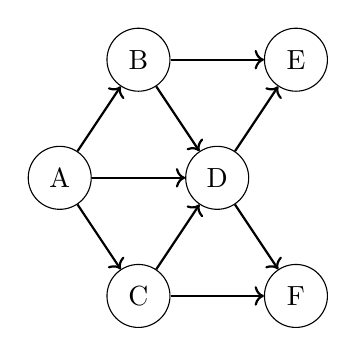
\begin{tikzpicture}[scale=0.5,
					every node/.style={circle, draw, minimum size=8mm}]
					\node (A) at (0,0) {A};
					\node (B) at (2,3) {B};
					\node (C) at (2,-3) {C};
					\node (D) at (4,0) {D};
					\node (E) at (6,3) {E};
					\node (F) at (6,-3) {F};
					\draw[->, thick] (A) to (B); 
					\draw[->, thick] (A) to	(D);  
					\draw[->, thick] (A) to (C); 
					\draw[->, thick] (B) to (D);
					\draw[->, thick] (C) to (D);
					\draw[->, thick] (B) to (E);
					\draw[->, thick] (C) to (F); 
					\draw[->, thick] (D) to (E);
					\draw[->, thick] (D) to (F);    
				\end{tikzpicture}
			\end{minipage}%
			\begin{minipage}{0.5\textwidth}
			BFS = A B C D E F \\
			BFS = A D B C F E \\
			BFS = A D B C E F \\
			\end{minipage}
		\end{center}
	\end{latin}
\end{answer}
پیمایش \lr{BFS} می تواند منحصر به فرد نباشد و شروع از هر گره دلخواه باشد.\\
فقط در زمان نوشتن پیمایش \lr{BFS} گراف جهت دار دقت شود که حرکت بین گره ها از طریق جهت یال ها انجام می شود.\\
\newline
\textbf{تابع پیمایش سطحی (\lr{BFS})}
\begin{flushright}
\begin{latin}
\begin{lstlisting}
bfs(v){
	front = rear = Null;
	cout<<v;
	visited[v] = True;
	addq(&front, &rear, v);
	while(front){
		v = deleteq(&front);
		for(w=graph[v];w;w=w->link);
		if(!visited[w->vertex]){
			cout<<w->vertex;
			addq(&front, &rear, w->vertex);
			visited[w->vertex] = True;}	
	}
}
\end{lstlisting}
\end{latin}
\end{flushright}

\newpage

\textbf{پیمایش عمقی}\\
با شروع از یک گره، آنرا ملاقات کرده و سپس کلیه گره های سمت چپ را تا آخرین عمق پیمایش میکنیم .\\
اگر در پایین رفتن های متوالی، گره ای ملاقات شود که هیچ گره همجواری نداشته باشد یا با تمام گره های همجوار آن ملاقات شده باشد، برگشت به یک سطح بالاتر  انجام می گیرد و روند فوق تکرار می شود.\\
پیمایش عمقی منحصر به فرد نیست.\\
\begin{latin}
	\begin{center}

\includegraphics[height=4cm,width=5cm]{graph1}
	\end{center}
\end{latin}
\begin{question}
یکی از پیمایش های \lr{DFS} گراف زیر را مشخص کنید.
\end{question}
\begin{answer}
با توجه به گراف داریم:
\begin{latin}
\begin{center}
\begin{tikzpicture}[scale=0.5,
					every node/.style={circle, draw, minimum size=8mm}]
					\node (A) at (0,4)  {A};
					\node (B) at (-2,2)  {B};
					\node (C) at (0,2) {C};
					\node (D) at (-4,0)  {D};
					\node (E) at (2,2)  {E};
					\node (F) at (-2,0) {F};
					\node (G) at (0,0) {G};
					\draw[--, thick] (D) to (B); 
					\draw[--, thick] (B) to	(A);  
					\draw[--, thick] (B) to (F); 
					\draw[--, thick] (B) to (D);
					\draw[--, thick] (A) to (C);
					\draw[--, thick] (A) to (E);
					\draw[--, thick] (C) to (G); 
					\draw[--, thick] (F) to [bend right=100] (E);   
\end{tikzpicture}
DFS = A B D F E C G\\
\end{center}
\end{latin}
\end{answer}

\begin{question}
	یکی از پیمایش های \lr{DFS} گراف زیر را مشخص کنید.
\end{question}
\begin{answer}
\begin{latin}
\begin{center}
\begin{minipage}{0.5\textwidth}
			\begin{tikzpicture}[scale=0.5,
				every node/.style={circle, draw, minimum size=8mm}]
				\node (a) at (2,6)  {a};
				\node (b) at (0,4) {b};
				\node (c) at (-2,2)  {c};
				\node (d) at (0,2) {d};
				\node (e) at (2,2)  {e};
				\node (f) at (5,2) {f};
				\node (g) at (0,0)  {g};
				\node (h) at (2,0) {h};
				\node (i) at (5,0)  {i};
				\draw[--, thick] (c) to (b); 
				\draw[--, thick] (c) to	(g);  
				\draw[--, thick] (b) to (d); 
				\draw[--, thick] (b) to (a);
				\draw[--, thick] (b) to (e);
				\draw[--, thick] (d) to (g);
				\draw[--, thick] (g) to (e); 
				\draw[--, thick] (g) to (h); 
				\draw[--, thick] (a) to (e);
				\draw[--, thick] (a) to (f);
				\draw[--, thick] (h) to (i);
				\draw[--, thick] (e) to (f); 
				\draw[--, thick] (e) to (i); 
				\draw[--, thick] (f) to (i);   
			\end{tikzpicture}
\end{minipage}%
\begin{minipage}{0.5\textwidth}
DFS = a b c g d e f i h\\
\end{minipage}
\end{center}
\end{latin}
\end{answer}

\newpage
\begin{question}
	سه پیمایش \lr{DFS} برای  گراف زیر را مشخص کنید.
\end{question}
\begin{answer}
\begin{latin}
\begin{center}
\begin{minipage}{0.5\textwidth}
			\begin{tikzpicture}[scale=0.5,
				every node/.style={circle, draw, minimum size=8mm}]
				\node (3) at (4,4)  {3};
				\node (2) at (2,4)  {2};
				\node (1) at (0,4)  {1};
				\node (6) at (4,2)  {6};
				\node (5) at (2,2)  {5};
				\node (4) at (0,2)  {4};
				\node (9) at (4,0)  {9};
				\node (8) at (2,0)  {8};
				\node (7) at (0,0)  {7};
				\draw[--, thick] (1) to (2); 
				\draw[--, thick] (1) to	(4);  
				\draw[--, thick] (2) to (3); 
				\draw[--, thick] (2) to (5);
				\draw[--, thick] (3) to (6);
				\draw[--, thick] (4) to (5);
				\draw[--, thick] (4) to (7); 
				\draw[--, thick] (5) to (6); 
				\draw[--, thick] (6) to (9);
				\draw[--, thick] (5) to (8);
				\draw[--, thick] (7) to (8);
				\draw[--, thick] (8) to (9); 	
\end{tikzpicture}
\end{minipage}%
\begin{minipage}{0.5\textwidth}
DFS = 1 2 3 6 9 8 7 4 5\\
DFS = 1 2 3 6 5 4 7 8 9\\
DFS = 1 4 7 8 9 6 5 2 3\\
\end{minipage}	
\end{center}
\end{latin}
\end{answer}
\begin{question}
	سه  پیمایش  \lr{BFS} گراف جهت دار زیر را بنویسید.
\end{question}
\begin{answer}
\begin{latin}
\begin{center}
\begin{minipage}{0.5\textwidth}
				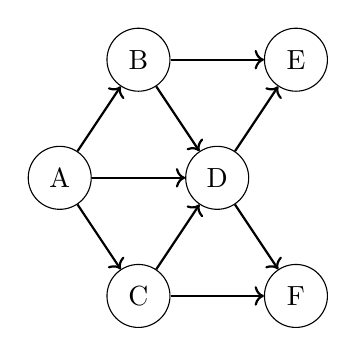
\begin{tikzpicture}[scale=0.5,
					every node/.style={circle, draw, minimum size=8mm}]
					\node (A) at (0,0) {A};
					\node (B) at (2,3) {B};
					\node (C) at (2,-3) {C};
					\node (D) at (4,0) {D};
					\node (E) at (6,3) {E};
					\node (F) at (6,-3) {F};
					\draw[->, thick] (A) to (B); 
					\draw[->, thick] (A) to	(D);  
					\draw[->, thick] (A) to (C); 
					\draw[->, thick] (B) to (D);
					\draw[->, thick] (C) to (D);
					\draw[->, thick] (B) to (E);
					\draw[->, thick] (C) to (F); 
					\draw[->, thick] (D) to (E);
					\draw[->, thick] (D) to (F);    
				\end{tikzpicture}
\end{minipage}%
\begin{minipage}{0.5\textwidth}
DFS = A B E D F C\\
DFS = A B D F E C\\
DFS = A D E F B C \\
\end{minipage}
\end{center}
\end{latin}
\end{answer}
\textbf{تابع پیمایش عمقی \lr{DFS}}\\
این تابع به دلیل بازگشتی بودن از پشته استفاده می کند.
\begin{flushright}
\begin{latin}
\begin{lstlisting}
dfs(v){
	visited[v] = True;
	cout<<v;
	for(w=graph[v];w;w=w->link)
		if(!visited[w->vertex])
			dfs(w->vertex);
}
\end{lstlisting}
\end{latin}
\end{flushright}
\newpage
\subsection{پیاده سازی گراف}

\textbf{پیاده سازی گراف با لیست  همجواری}\\

\begin{latin}
	\begin{minipage}{0.45\textwidth}
		\centering
\begin{lstlisting}
int main(){
	int v = 5;
	struct Graph* g;
	g = createGraph(v);
	addEdge(g, 0, 1);
	addEdge(g, 0, 4);
	addEdge(g, 1, 2);
	addEdge(g, 1, 3);
	addEdge(g, 1, 4);
	addEdge(g, 2, 3);
	addEdge(g, 3, 4);
	printGraph(g)
}
\end{lstlisting}
	\end{minipage}%
	\hfill
	\begin{minipage}{0.6\textwidth}
					\begin{tikzpicture}[scale=0.5,
		every node/.style={circle, draw, minimum size=8mm}]
		\node (4) at (0,0) {4};
		\node (0) at (0,4) {0};
		\node (3) at (4,0) {3};
		\node (1) at (4,4) {1};
		\node (2) at (6,2) {2};
		\draw[--, thick] (0) to (1); 
		\draw[--, thick] (0) to	(4);  
		\draw[--, thick] (4) to (1); 
		\draw[--, thick] (4) to (3);
		\draw[--, thick] (3) to (1);
		\draw[--, thick] (3) to (2);
		\draw[--, thick] (1) to (2); 
	\end{tikzpicture}
	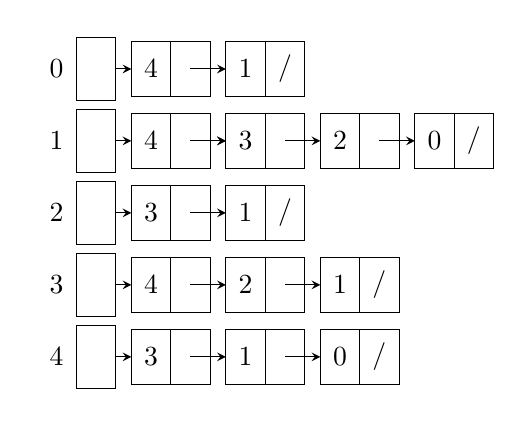
\begin{tikzpicture}[>=stealth] 
	\matrix (M) [matrix of nodes,% 
	column sep=-\pgflinewidth,% 
	row sep=1mm,% 
	nodes in empty cells,
	nodes={draw,%
		minimum width=.5cm, outer sep=0pt,% 
		minimum height=.7cm, anchor=center}, 
	column 1/.style={nodes={minimum height=.8cm}}]%
	{ 
		|[label=left:0]| &[2mm] 4 & &[2mm] 1 & /  \\ 
		|[label=left:1]| &[2mm] 4 & &[2mm] 3 &&[2mm] 2 & &[2mm] 0  & / \\ 
		|[label=left:2]| &[2mm] 3 & &[2mm] 1 & / \\ 
		|[label=left:3]| &[2mm] 4 & &[2mm] 2 & &[2mm] 1 & /  \\ 
		|[label=left:4]| &[2mm] 3 & &[2mm] 1 & &[2mm] 0 & /    \\
	}; 
	
	\foreach \i in {1,2,3,4,5}{ 
		\draw[->] (M-\i-1)--(M-\i-2.west); 
		\draw[->] (M-\i-3.center)--(M-\i-4.west);
	}
	\draw[->] (M-2-5.center)--(M-2-6.west); 
	\draw[->] (M-2-7.center)--(M-2-8.west); 
	\draw[->] (M-2-3.center)--(M-2-4.west); 
	\draw[->] (M-4-5.center)--(M-4-6.west); 
	\draw[->] (M-5-5.center)--(M-5-6.west); 
\end{tikzpicture} 
\newline
\end{minipage}
\end{latin}
\newline
\textbf{تعریف استراکچر ها}\\

\begin{latin}
\begin{minipage}{0.45\textwidth}
		\centering
\begin{lstlisting}
struct Node{
	int data;
	struct Node* next;
}
\end{lstlisting}
\begin{lstlisting}
struct AdjList{
	struct Node* head;
}
\end{lstlisting}
\begin{lstlisting}
struct Graph{
	int v;
	struct AdjList* array;
}
\end{lstlisting}
	\end{minipage}%
	\hfill
	\begin{minipage}{0.6\textwidth}
		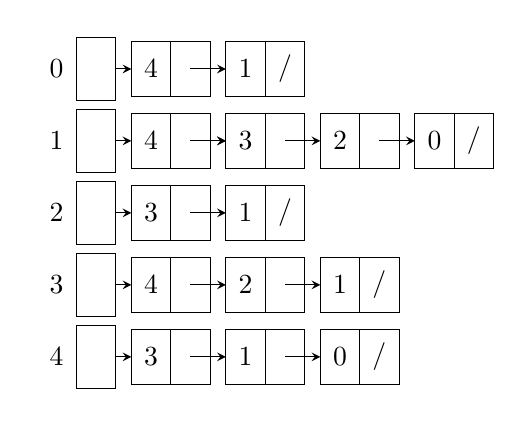
\begin{tikzpicture}[>=stealth] 
			\matrix (M) [matrix of nodes,% 
			column sep=-\pgflinewidth,% 
			row sep=1mm,% 
			nodes in empty cells,
			nodes={draw,%
				minimum width=.5cm, outer sep=0pt,% 
				minimum height=.7cm, anchor=center}, 
			column 1/.style={nodes={minimum height=.8cm}}]%
			{ 
				|[label=left:0]| &[2mm] 4 & &[2mm] 1 & /  \\ 
				|[label=left:1]| &[2mm] 4 & &[2mm] 3 &&[2mm] 2 & &[2mm] 0  & / \\ 
				|[label=left:2]| &[2mm] 3 & &[2mm] 1 & / \\ 
				|[label=left:3]| &[2mm] 4 & &[2mm] 2 & &[2mm] 1 & /  \\ 
				|[label=left:4]| &[2mm] 3 & &[2mm] 1 & &[2mm] 0 & /    \\
			}; 
			
			\foreach \i in {1,2,3,4,5}{ 
				\draw[->] (M-\i-1)--(M-\i-2.west); 
				\draw[->] (M-\i-3.center)--(M-\i-4.west);
			}
			\draw[->] (M-2-5.center)--(M-2-6.west); 
			\draw[->] (M-2-7.center)--(M-2-8.west); 
			\draw[->] (M-2-3.center)--(M-2-4.west); 
			\draw[->] (M-4-5.center)--(M-4-6.west); 
			\draw[->] (M-5-5.center)--(M-5-6.west); 
		\end{tikzpicture} 
	\end{minipage}
\end{latin}
\newpage

\textbf{ایجاد یک گره}\\
\begin{flushright}
\begin{latin}
\begin{lstlisting}
struct Node* newNode(int a){
	struct Node* n;
	n = malloc(sizeof(struct Node));
	n->data = Null;
	n->next = Null;
	return n;
}
\end{lstlisting}
\end{latin}
\end{flushright}
\textbf{ساخت گراف }\\
\begin{latin}
	\begin{minipage}{0.6\textwidth}
		\centering
\begin{lstlisting}
struct Graph* createGraph(int v){
	struct Graph* g;
	g= malloc(sizeof(structGraph));
	g->v = v;
	g->array = malloc(v * sizeof(structAdjList));
	int i;
	for(i=0;i<v;++i){
		g->array[i].head = Null;}
	retrun g;
}			
\end{lstlisting}
	\end{minipage}%
	\hfill
	\begin{minipage}{0.3\textwidth}
		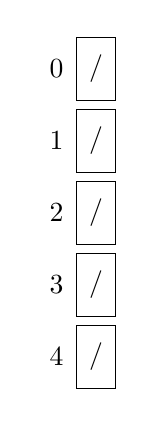
\begin{tikzpicture}[>=stealth] 
	\matrix (M) [matrix of nodes,% 
	column sep=-\pgflinewidth,% 
	row sep=1mm,% 
	nodes in empty cells,
	nodes={draw,%
		minimum width=.5cm, outer sep=0pt,% 
		minimum height=.7cm, anchor=center}, 
	column 1/.style={nodes={minimum height=.8cm}}]%
	{ 
		|[label=left:0]|  / \\ 
		|[label=left:1]|  / \\ 
		|[label=left:2]|  / \\ 
		|[label=left:3]|  / \\ 
		|[label=left:4]|  / \\
	}; 
\end{tikzpicture} 
	\end{minipage}
\end{latin}
\newpage

\textbf{اضافه کردن یال}
\begin{latin}
	\begin{minipage}{0.6\textwidth}
		\centering
\begin{lstlisting}
void addEdge(struct Graph* g, int s, int d){
	
	// Add an edge from source to dest.
	
	struct Node* n = newNode(d);
	n->next = f->array[s].head;
	g->array[s].head = n;
	
	// Since the graph is undirected, add an edge from dest to source also
	
	n = newNode(s);
	n->next = g->array[d].head;
	g->array[d].head = n;}		
\end{lstlisting}
	\end{minipage}%
	\hfill
	\begin{minipage}{0.3\textwidth}
			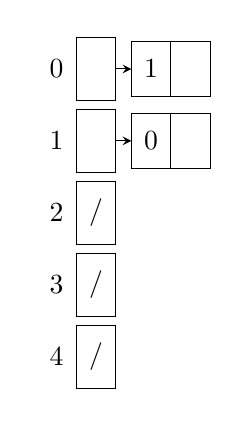
\begin{tikzpicture}[>=stealth] 
		\matrix (M) [matrix of nodes,% 
		column sep=-\pgflinewidth,% 
		row sep=1mm,% 
		nodes in empty cells,
		nodes={draw,%
			minimum width=.5cm, outer sep=0pt,% 
			minimum height=.7cm, anchor=center}, 
		column 1/.style={nodes={minimum height=.8cm}}]%
		{ 
			|[label=left:0]| &[2mm] 1 &   \\ |[label=left:1]| &[2mm] 0 &  \\ 
			|[label=left:2]|  / \\ 
			|[label=left:3]|  / \\ 
			|[label=left:4]|  / \\ 	
		}; 
		\draw[->] (M-1-1)--(M-1-2.west); 	
		\draw[->] (M-2-1)--(M-2-2.west);
	\end{tikzpicture} 
	\end{minipage}
\end{latin}
\textbf{چاپ گراف}\\

\begin{latin}
	\begin{minipage}{0.6\textwidth}
		\centering
\begin{lstlisting}
void printGraph(struct Graph* g)
{
	int i;
	struct Node* p;
	for(i=0;i<g->v;++i)
	{
		p = g->array[i].head;
		printf("vertex %d:",i);
		while(p){
		   printf("-> %d",p->data);
		   p = p->next;	
				}
		printf("\n");	
	}
}
\end{lstlisting}
	\end{minipage}%
	\hfill
	\begin{minipage}{0.3\textwidth}
		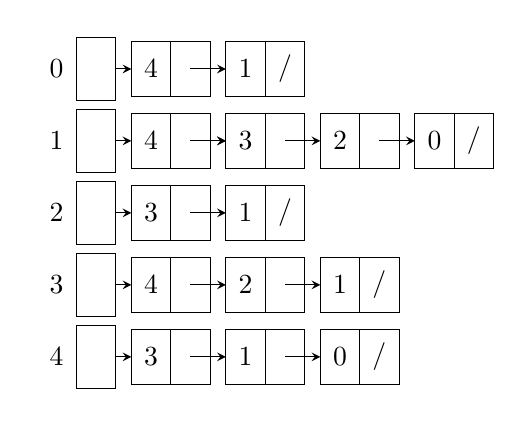
\begin{tikzpicture}[>=stealth] 
	\matrix (M) [matrix of nodes,% 
	column sep=-\pgflinewidth,% 
	row sep=1mm,% 
	nodes in empty cells,
	nodes={draw,%
		minimum width=.5cm, outer sep=0pt,% 
		minimum height=.7cm, anchor=center}, 
	column 1/.style={nodes={minimum height=.8cm}}]%
	{ 
		|[label=left:0]| &[2mm] 4 & &[2mm] 1 & /  \\ 
		|[label=left:1]| &[2mm] 4 & &[2mm] 3 &&[2mm] 2 & &[2mm] 0  & / \\ 
		|[label=left:2]| &[2mm] 3 & &[2mm] 1 & / \\ 
		|[label=left:3]| &[2mm] 4 & &[2mm] 2 & &[2mm] 1 & /  \\ 
		|[label=left:4]| &[2mm] 3 & &[2mm] 1 & &[2mm] 0 & /    \\
	}; 
	
	\foreach \i in {1,2,3,4,5}{ 
		\draw[->] (M-\i-1)--(M-\i-2.west); 
		\draw[->] (M-\i-3.center)--(M-\i-4.west);
	}
	\draw[->] (M-2-5.center)--(M-2-6.west); 
	\draw[->] (M-2-7.center)--(M-2-8.west); 
	\draw[->] (M-2-3.center)--(M-2-4.west); 
	\draw[->] (M-4-5.center)--(M-4-6.west); 
	\draw[->] (M-5-5.center)--(M-5-6.west); 
\end{tikzpicture} 
\begin{footnotesize}
\underline{On screen}:\\
	vertex0: -> 4 -> 1\\
	vertex1: -> 4 -> 3 -> 2 -> 0\\
	vertex2: -> 3 -> 1\\
	vertex3: -> 4 -> 2 -> 1\\
	vertex4: -> 3 -> 1 -> 0 \\
\end{footnotesize}
	\end{minipage}
\end{latin}

\newpage

\section{مرتب سازی}
الگوریتم های مرتب سازی را از نظر نحوه مرتب سازی می توان به دو دسته تقسیم کرد.
\begin{enumerate}
	\item 
مرتب سازی مبتی بر مقایسه \lr{(Comparison based)}:\\
با مقایسه بین کلیه عناصر، ترتیب نسبی آنها پیدا می شود.
	\item 
مرتب سازی غیر مقایسه ای یا خطی \lr{(Non-Comparison based)}:\\
بدون مقایسه کلیه عناصر با هم، عمل مرتب سازی انجام می شود.
\end{enumerate}

الگوریتم های مرتب سازی مقایسه ای:
\begin{itemize}
	\item حبابی \lr{(Bubble)}
	\item درجی  \lr{(Insertion)}
	\item سریع  \lr{(Quick)}
	\item درختی \lr{(Tree)}
	\item انتخابی \lr{(Selection)}
	\item ادغامی \lr{(Merge)}
	\item هیپ \lr{(Heap)}
	\item شل \lr{(Shell)}
\end{itemize}


الگوریتم های مرتب سازی غیر مقایسه ای:
\begin{itemize}
	\item شمارشی \lr{(Count)}
	\item سطلی \lr{(Bucket sort)}
	\item مبنایی \lr{(Radix sort)}
	\item لانه کبوتری
\end{itemize}

در این درس فقط به بررسی سه الگوریتم حبابی، درجی و انتخابی خواهیم پرداخت.\\
\newpage
\subsection{مرتب سازی حبابی}
در این روش با چند بار حرکت در طول آرایه، یک عنصر با عنصر بعدی مقایسه شده و در صورت لزوم جابه جا می شود.\\
به عنوان مثال برای بررسی عملکرد مرتب سازی حبابی آرایه ای به صورت \lr{(5, 1, 4, 2, 8)} داریم، مراحل مرتب سازی حبابی برای این آرایه به صورت زیر است.\\
\begin{center}
\begin{tabular}{c c}
\lr{(5, 1, 4, 2, 8)} & 
مقدار آرایه به عنوان ورود به الگوریتم داده می شود.\\
\lr{(1, 5, 4, 2, 8)}  & 
در  گام اول ، عدد ۵ و ۱ با هم مقایسه شده و در نتیجه جای این مقدار با هم عوض می شود.\\
\lr{(1, 4, 5, 2, 8)}  & 
در گام دوم ، دو مقدار ۵ و۴ باهم مقایسه می شوند و در نتیجه جای این دو مقدار در آرایه نیز با هم عوض می شود.\\
\lr{(1, 4, 2, 5, 8)}  &
 در گام سوم ، عدد ۲ تا ۵ مقایسه شده و به دلیل بزرگتر بودن ۵ جای این دو مقدار نیز باهم عوض می شود.\\
\lr{(1, 4, 2, 5, 8)}  & 
در نهایت دو مقدار ۸ و ۵ را با هم مقایسه کرده که در نتیجه نیاز به تعویض نداریم.\\
 & حال باید به مرحله دوم مرتب سازی برویم (فاز۲)\\
\lr{(1, 4, 2, 5, \underline{8})}&
 در این مرحله نیز  دقیقا همانند مرحله اول، مقایسه عناصر را با هم مقایسه میکنیم .\\
\lr{(1, 2, 4, 5, \underline{8})}&
 با تعویض خانه دو عنصر ۲و۴ باهم به فرم نهایی رسید و مرتب سازی به اتمام خواهد رسید.\\
\end{tabular}
\end{center}
در هر مرحله ای که در مرتب سازی حبابی طی می شود، یک عنصر از آخر لیست برای مقایسه نشدن ،حذف می شود.(لیست تغییر نمی کند بلکه بازه مقایسه ماست که کوچک می شود.)\\
همچنین با ایجاد یک \lr{flag} می توانیم این الگوریتم را هوشمند کنیم ، درصورتیکه  عمل \lr{swap} در مرحله ای انجام نشد ، دیگر ادامه نده .\\
\begin{question}
با کمک مرتب سازی حبابی آرایه زیر را مرتب کنید:
\lr{(8, 4, 3, 2)}
\end{question}
\begin{answer}
\begin{center}
\begin{tabular}{c c}
مرحله مرتب سازی & وضعیت عناصر در آرایه\\
&\\
\lr{(1)} & \lr{(8, 4, 3, 2)} \\
& \lr{(4, 8, 3, 2)}\\
& \lr{(4, 3, 8, 2)}\\
& \lr{(4, 3, 2, 8)}\\
&\\
\lr{(2)} & \lr{(3, 4, 2, \underline{8})}\\
& \lr{(3, 2, 4, \underline{8})}\\
&\\
\lr{(3)} & \lr{(2, 3, \underline{4}, \underline{8})}\\
\end{tabular}
\end{center}
\end{answer}
\newpage

\textbf{الگوریتم مرتب سازی حبابی}\\
\begin{flushright}
\begin{latin}
\begin{lstlisting}
void bubblesort(int arr[], int n){
	int i,j;bool swapped;
	for(i=0;i<n-1;i++){
		swapped = false;
		for(j=0;j<n-i-1;j++){
			if(arr[j]>arr[j+1]){
				swap(&arr[j], &arr[j+1]);
				swapped = True;}	
			}
		if(swappped == false) break;
	}
}
\end{lstlisting}
\end{latin}
\end{flushright}

\subsection{مرتب سازی انتخابی}
قرار دادن کوچکترین عنصر آرایه در مکان اول آرایه\\
قرار دادن کوچکترین عنصر دوم آرایه در مکان دوم آرایه و به همین ترتیب برای تمام عناصر.\\
به طور مثال برای آرایه \lr{(10, 30, 17, 12, 1, 21, 15)}
مرتب سازی انتخابی به صورت زیر می باشد:\\
\newline

\begin{latin}
\centering
\begin{tabular}{c c c c c c c}
10 & 30 & 17 & 12 & 1 & 21 & 15\\
\underline{1} & 30 & 17 & 12 & 10 & 21 & 15\\
\underline{1} & \underline{10} & 17 & 12 & 30 & 21 & 15\\
\underline{1} & \underline{10} & \underline{12} & 17 & 30 & 21 & 15\\
\underline{1} & \underline{10} & \underline{12} & \underline{15} & 30 & 21 & 17\\
\underline{1} & \underline{10} & \underline{12} & \underline{15}& \underline{17} & 21 & 30\\
\underline{1} & \underline{10} & \underline{12} & \underline{15}& \underline{17} & \underline{21} & \underline{30}\\
\end{tabular}\\
\end{latin}\\

\newline
اگر در روش انتخابی به جای کوچکترین عنصر، بزرگترین عنصر را پیدا کنیم، آنگاه لیست ما به صورت نزولی در خواهد آمد.\\
برای \lr{n} عنصر \lr{n-1} مرحله در مرتب سازی انتخابی داریم.\\
الگوریتم حبابی و انتخابی هر دو دارای مرتبه اجرایی $n^2$
می باشد.\\
\newpage
\textbf{الگوریتم مرتب سازی انتخابی}
\begin{flushright}
\begin{latin}
\begin{lstlisting}
void selectionSort(int arr[], int n){
	int i,j,m;
	for(i=0;i<n-1;i++){
		m = i;
		for(j=j+1;j<n;j++){
			if(arr[j]<arr[m])	
				m = j;
			}
		swap(&arr[m], &arr[i]);	
	}
}
\end{lstlisting}
\end{latin}
\end{flushright}

\subsection{مرتب سازی درجی}
با فرض اینکه عدد اول در لیست در جای درستی قرار گرفته است عدد دوم را با آن مقایسه می کنیم، اگر کوچک تر بود جابه جا شود ، سپس عدد سوم را با دو عددی که با هم مقایسه کرده ایم بررسی میکنیم و به همین ترتیب.\\
\begin{latin}
	\centering
\begin{tabular}{c c c c c c c c}
\underline{8} & 5 & 3 & 21 & 12 & 11 & 6 & 2\\
\underline{5} & \underline{8} & 3 & 21 & 12 & 11 & 6 & 2\\
\underline{3} & \underline{5} & \underline{8} & 21 & 12 & 11 & 6 & 2\\
\underline{3} & \underline{5} & \underline{8} & \underline{21} & 12 & 11 & 6 & 2\\
\underline{3} & \underline{5} & \underline{8} & \underline{12} & \underline{21} & 11 & 6 & 2\\
\underline{3} & \underline{5} & \underline{8} & \underline{11} & \underline{12} & \underline{21} & 6 & 2\\
\underline{3} & \underline{5} & \underline{6} & \underline{8} & \underline{11} & \underline{12} & \underline{21} & 2\\
\underline{2} & \underline{3} & \underline{5} & \underline{6} & \underline{8} & \underline{11} & \underline{12} & \underline{21}\\
\end{tabular}\\
\end{latin}\\
\newpage

\textbf{الگوریتم مرتب سازی درجی}\\
\begin{flushright}
	\begin{latin}
\begin{lstlisting}
void insertionSort(int arr[], int n){
	int i,key,j;
	for(i=1;i<n;i++){
		key = arr[i]	
		j = i-1;
		while(j>=0 && arr[j]>key){
			arr[j+1] = arr[j];
			j = j-1;	
		}
		arr[j+1] = key;
	}
}
\end{lstlisting}
	\end{latin}
\end{flushright}




\end{document}
